%%
%% This is file `sample-sigconf.tex',
%% generated with the docstrip utility.
%%
%% The original source files were:
%%
%% samples.dtx  (with options: `all,proceedings,bibtex,sigconf')
%% 
%% IMPORTANT NOTICE:
%% 
%% For the copyright see the source file.
%% 
%% Any modified versions of this file must be renamed
%% with new filenames distinct from sample-sigconf.tex.
%% 
%% For distribution of the original source see the terms
%% for copying and modification in the file samples.dtx.
%% 
%% This generated file may be distributed as long as the
%% original source files, as listed above, are part of the
%% same distribution. (The sources need not necessarily be
%% in the same archive or directory.)
%%
%%
%% Commands for TeXCount
%TC:macro \cite [option:text,text]
%TC:macro \citep [option:text,text]
%TC:macro \citet [option:text,text]
%TC:envir table 0 1
%TC:envir table* 0 1
%TC:envir tabular [ignore] word
%TC:envir displaymath 0 word
%TC:envir math 0 word
%TC:envir comment 0 0
%%
%%
%% The first command in your LaTeX source must be the \documentclass
%% command.
%%
%% For submission and review of your manuscript please change the
%% command to \documentclass[manuscript, screen, review]{acmart}.
%%
%% When submitting camera ready or to TAPS, please change the command
%% to \documentclass[sigconf]{acmart} or whichever template is required
%% for your publication.
%%
%%
\documentclass[sigconf, natbib=false]{acmart}

%%
%% \BibTeX command to typeset BibTeX logo in the docs
% \AtBeginDocument{%
%   \providecommand\BibTeX{{%
%     Bib\TeX}}}

%% Rights management information.  This information is sent to you
%% when you complete the rights form.  These commands have SAMPLE
%% values in them; it is your responsibility as an author to replace
%% the commands and values with those provided to you when you
%% complete the rights form.
% \setcopyright{acmlicensed}
% \copyrightyear{2018}
% \acmYear{2018}
% \acmDOI{XXXXXXX.XXXXXXX}

%% These commands are for a PROCEEDINGS abstract or paper.
% \acmConference[Conference acronym 'XX]{Make sure to enter the correct
%   conference title from your rights confirmation emai}{June 03--05,
%   2018}{Woodstock, NY}
%%
%%  Uncomment \acmBooktitle if the title of the proceedings is different
%%  from ``Proceedings of ...''!
%%
%%\acmBooktitle{Woodstock '18: ACM Symposium on Neural Gaze Detection,
%%  June 03--05, 2018, Woodstock, NY}
% \acmISBN{978-1-4503-XXXX-X/18/06}


%%
%% Submission ID.
%% Use this when submitting an article to a sponsored event. You'll
%% receive a unique submission ID from the organizers
%% of the event, and this ID should be used as the parameter to this command.
%%\acmSubmissionID{123-A56-BU3}

%%
%% For managing citations, it is recommended to use bibliography
%% files in BibTeX format.
%%
%% You can then either use BibTeX with the ACM-Reference-Format style,
%% or BibLaTeX with the acmnumeric or acmauthoryear sytles, that include
%% support for advanced citation of software artefact from the
%% biblatex-software package, also separately available on CTAN.
%%
%% Look at the sample-*-biblatex.tex files for templates showcasing
%% the biblatex styles.
%%

%%
%% The majority of ACM publications use numbered citations and
%% references.  The command \citestyle{authoryear} switches to the
%% "author year" style.
%%
%% If you are preparing content for an event
%% sponsored by ACM SIGGRAPH, you must use the "author year" style of
%% citations and references.
%% Uncommenting
%% the next command will enable that style.
%%\citestyle{acmauthoryear}
\usepackage[backend=bibtex]{biblatex}
\addbibresource{honors.bib}

%%
%% end of the preamble, start of the body of the document source.
\begin{document}

%%
%% The "title" command has an optional parameter,
%% allowing the author to define a "short title" to be used in page headers.
\title{An Evaluation of Deep-Q-Learning methods on the Hanabi Challenge}

%%
%% The "author" command and its associated commands are used to define
%% the authors and their affiliations.
%% Of note is the shared affiliation of the first two authors, and the
%% "authornote" and "authornotemark" commands
%% used to denote shared contribution to the research.
\author{Kival R. Mahadew}
\email{221001688@stu.ukzn.ac.za}
\orcid{0009-0008-1712-5746}
\affiliation{%
  \institution{University of KwaZulu-Natal}
  \city{Durban}
  \state{KwaZulu-Natal}
  \country{South Africa}
}


%%
%% By default, the full list of authors will be used in the page
%% headers. Often, this list is too long, and will overlap
%% other information printed in the page headers. This command allows
%% the author to define a more concise list
%% of authors' names for this purpose.
\renewcommand{\shortauthors}{Mahadew}

%%
%% The abstract is a short summary of the work to be presented in the
%% article.
\begin{abstract}
    The card game Hanabi presents a complex, cooperative, multi-agent problem that emphasizes communication and strategy within a partially observable environment. The challenges in developing Hanabi playing agents are similar to many real-world applications requiring efficient cooperation, from self-driving cars to virtual assistants. The importance of understanding how agents can effectively cooperate in such environments has become increasingly important. This paper evaluated the performance of deep-Q-learning techniques, focusing specifically on the Rainbow DQN and Simplified Action Decoder agents, in the cooperative multi-agent environment of Hanabi. The performance of the deep-Q-learning agents are compared in the two-player setting of Hanabi, focusing on their sample efficiency and generalization to unseen partners. Our results show that the Rainbow and the Simplified Action Decoder agents outperform the other agents in the two-player self-play version of Hanabi. Our findings highlight the importance of the Rainbow DQN components in achieving high performance in Hanabi and the importance of the Simplified Action Decoder in stabilizing the learning process and improving the performance of the agents.  Additionally, we find that independently trained agents struggle to cooperate effectively with agents that they have not been trained with. This study contributes insights into the development of more robust and collaborative MARL systems, offering a foundation for future research in similar multi-agent cooperative domains.
\end{abstract}

%%
%% The code below is generated by the tool at http://dl.acm.org/ccs.cfm.
%% Please copy and paste the code instead of the example below.
%%
% \begin{CCSXML}
% <ccs2012>
%  <concept>
%   <concept_id>00000000.0000000.0000000</concept_id>
%   <concept_desc>Do Not Use This Code, Generate the Correct Terms for Your Paper</concept_desc>
%   <concept_significance>500</concept_significance>
%  </concept>
%  <concept>
%   <concept_id>00000000.00000000.00000000</concept_id>
%   <concept_desc>Do Not Use This Code, Generate the Correct Terms for Your Paper</concept_desc>
%   <concept_significance>300</concept_significance>
%  </concept>
%  <concept>
%   <concept_id>00000000.00000000.00000000</concept_id>
%   <concept_desc>Do Not Use This Code, Generate the Correct Terms for Your Paper</concept_desc>
%   <concept_significance>100</concept_significance>
%  </concept>
%  <concept>
%   <concept_id>00000000.00000000.00000000</concept_id>
%   <concept_desc>Do Not Use This Code, Generate the Correct Terms for Your Paper</concept_desc>
%   <concept_significance>100</concept_significance>
%  </concept>
% </ccs2012>
% \end{CCSXML}

% \ccsdesc[500]{Do Not Use This Code~Generate the Correct Terms for Your Paper}
% \ccsdesc[300]{Do Not Use This Code~Generate the Correct Terms for Your Paper}
% \ccsdesc{Do Not Use This Code~Generate the Correct Terms for Your Paper}
% \ccsdesc[100]{Do Not Use This Code~Generate the Correct Terms for Your Paper}

%%
%% Keywords. The author(s) should pick words that accurately describe
%% the work being presented. Separate the keywords with commas.
\keywords{Hanabi, Deep Q-Learning, Multi-Agent Systems, Reinforcement Learning}
%% A "teaser" image appears between the author and affiliation
%% information and the body of the document, and typically spans the
%% page.
% \begin{teaserfigure}
% %   \includegraphics[width=\textwidth]{sampleteaser}
%   \caption{Seattle Mariners at Spring Training, 2010.}
%   \Description{Enjoying the baseball game from the third-base
%   seats. Ichiro Suzuki preparing to bat.}
%   \label{fig:teaser}
% \end{teaserfigure}

% \received{20 February 2007}
% \received[revised]{12 March 2009}
% \received[accepted]{5 June 2009}

%%
%% This command processes the author and affiliation and title
%% information and builds the first part of the formatted document.
\maketitle

\section{Introduction}
Cooperation is a fundamental aspect of human society. It is the foundation of social structures, economies, and even the evolution of species. Cooperation involves working together in teams to achieve a common goal and sharing resources and information with others. Cooperation is essential for solving complex problems that require the coordination of multiple agents, each with its own goals and objectives. Human beings are naturally adept at cooperating with others, even with challenges such as limited information, communication barriers, and conflicting interests.

Cooperation is a challenging problem in artificial intelligence and has been studied extensively \cite{yuanSurveyProgressCooperative2023}. The ability of agents to cooperate effectively can lead to significant improvements in performance and efficiency. However, cooperation is not always straightforward, especially when agents have limited information about their environment or the other agents they are interacting with. Despite these challenges, significant progress has been made in developing algorithms that enable agents to cooperate in a variety of settings \cite{huSimplifiedActionDecoder2021, liACECooperativeMultiagent2022}.

The game of Hanabi has emerged as a popular benchmark for evaluating the performance of cooperative multi-agent systems. Hanabi is a cooperative card game where players work together to build sets of cards in a specific order. Players have limited information about their own cards and must rely on communication and reasoning to infer their cards from other players' actions. Hanabi's combination of cooperative gameplay, dynamic environments, imperfect information, and reliance on theory of mind reasoning makes it a challenging benchmark for evaluating the performance of computational multi-agents in playing the game \cite{bardHanabiChallengeNew2020a}. Human players have been shown to outperform AI agents by a large margin; even first-time players can easily understand the game and perform well \cite{sidjiHiddenRulesHanabi2023, ArtificialIntelligenceSmart2021}. This makes Hanabi an interesting benchmark for automated game playing. 

A large number of attempts have been made to develop automated players using deep reinforcement learning. Deep reinforcement learning is a sub-field of artificial intelligence that combines deep learning techniques with reinforcement learning to learn complex policies from high-dimensional input data. Deep reinforcement learning algorithms use neural networks to learn a mapping from environmental states to actions. The agent learns to attempt to maximize a reward signal that is provided by the environment. Deep reinforcement learning has been successful in learning to play complex games such as Go \cite{AlphaGoGoogleDeepMind} and StarCraft 2 \cite{googleAlphaStarMasteringRealtime2019}, control autonomous vehicles \cite{bhallaDeepMultiAgent2020}, and solve a variety of sequential decision-making problems \cite{mnihPlayingAtariDeep2013}.

Deep Multi-Agent Reinforcement Learning (MARL) has shown promise in addressing the challenges of cooperation in multi-agent systems. MARL combines deep learning techniques with reinforcement learning in multi-agent settings to enable agents to learn to cooperate effectively in complex and dynamic environments. Recent advances in MARL have led to significant improvements in the performance of agents in cooperative settings, including Hanabi \cite{huOtherPlayZeroShotCoordination, foersterBayesianActionDecoder2019}. However, there are still many open questions and challenges in the field of MARL, particularly in the context of cooperation with new partners, efficient exploration, and sample efficiency \cite{dafoeOpenProblemsCooperative2020, canaanDiverseAgentsAdHoc2019, bardHanabiChallengeNew2020a}.

Deep-Q-learning reinforcement learning techniques, specifically, have shown state-of-the-art performance in Hanabi, with the Rainbow DQN and Simplified Action Decoder agents achieving superhuman performance in self-play \cite{huSimplifiedActionDecoder2021, bardHanabiChallengeNew2020a}. However, their performance in Hanabi has not yet been fully explored. 

This project aims to evaluate the performance of deep-Q-learning techniques in Hanabi's cooperative multi-agent environment. We focus specifically on the Rainbow DQN and Simplified Action Decoder agents. We compare the performance of these agents to simple DQN agents in the two-player setting of Hanabi, focusing on their sample efficiency, exploration and generalization to unseen partners. Our goal is to identify the key factors that contribute to the success of these algorithms in Hanabi and to provide insights into how they can be further improved.

The paper is structured as follows: Section 2 provides a background on Hanabi and the challenges it presents for learning agents, as well as reinforcement learning and deep-Q-learning techniques. Section 3 provides an overview of literature surrounding Hanabi and cooperative MARL. Section 4 describes the methods used in this study, including the experimental setup, agents, training setup, and evaluation metrics. Section 5 presents the results of the experiments and discusses the performance of the agents. Section 6 provides a conclusion and discusses the implications of the findings for future research in cooperative MARL.
\section{Background}
\subsection{Hanabi}

The Hanabi Challenge has become a popular benchmark in MARL due to its unique properties as a cooperative, partially observable game where players must deduce each other's intentions to succeed. Unlike many competitive MARL tasks, Hanabi requires long-term strategies and implicit communication, posing unique challenges for traditional and deep reinforcement learning algorithms.
\paragraph*{Gameplay}
Hanabi is a cooperative card game of two to five players working together to achieve a common goal. It is often described as a form of cooperative solitaire. The game is played with a deck of cards, each with a colour and a number. The game's goal is to play cards in ascending order for each colour, starting from 1 to 5. Players can only see the cards of other players but have to infer the cards in their hands from the actions of other players. Players can give hints to each other about the cards in their hands, but they are limited in the number of hints they can give, they can also play cards but lose a life if they play a card incorrectly, and they can discard cards to gain more hints.
The game ends when the deck is empty, or the number of incorrect plays reaches a certain threshold. The players' score is determined by the number of cards played correctly by the end of the game, or 0 if the game ends due to too many incorrect plays.

\begin{figure}[h]
    \centering
    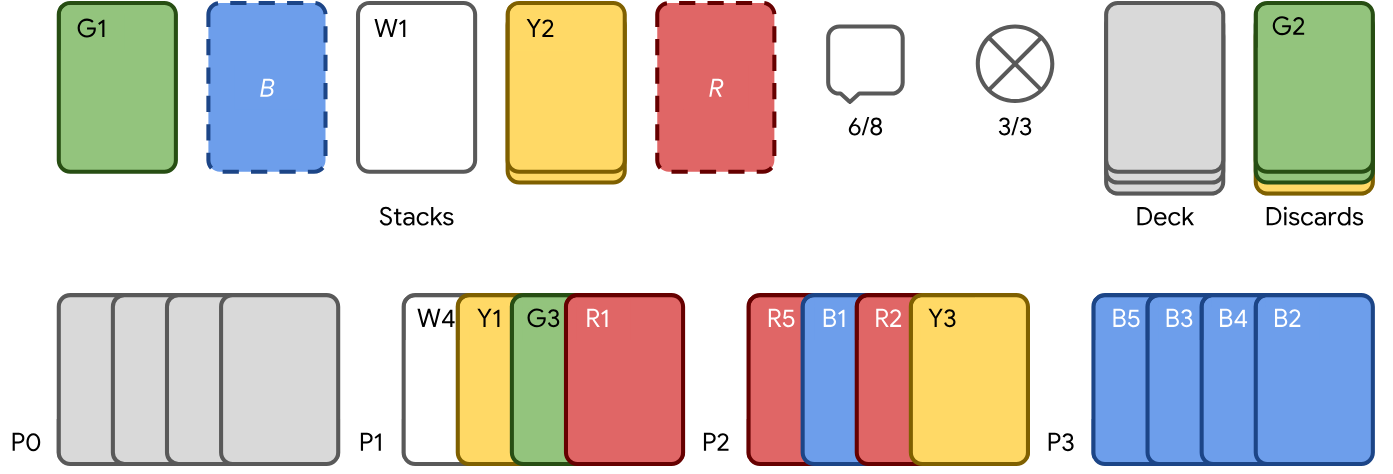
\includegraphics[width=\linewidth]{images/Hanabi.png}
    \caption{
      Four player Hanabi gameplay from the perspective of Player 0. The player can see the cards of other players but not their own, and the goal is to play cards in ascending order for each colour. This image is taken from the Hanabi Challenge paper \cite{bardHanabiChallengeNew2020a}
    }
    \Description{Training curve for Rainbow Agent}
  \end{figure}

\paragraph*{Challenges}
Hanabi was first presented as a challenge for AI research as early as 2015 by \textcite{osawaSolvingHanabiEstimating2015} to serve as a benchmark for evaluating the imitation of human intelligence with artificial intelligence. The work showcased strategies that attempted to recognize intent and infer hidden information to achieve high scores in Hanabi. The first rule-based approaches appeared later that year by \textcite{coxHowMakePerfect2015}. Since then, several deep-reinforcement learning algorithms have been developed to play Hanabi, achieving superhuman performance \cite{huSimplifiedActionDecoder2021, canaanEvaluatingRlAgents2020, foersterBayesianActionDecoder2019}.
Hanabi presents several challenges for MARL algorithms. The game is partially observable, meaning that players can only see the cards of other players and have to infer the cards in their hands from the actions of other players. This requires agents to develop theory-of-mind reasoning to infer the intentions of other players. The game also requires long-term planning and coordination between players, as the actions of one player affect the actions of other players. Finally, the game is stochastic, as the deck is shuffled at the beginning of each game, and the actions of other players can be unpredictable.
\textcite{bardHanabiChallengeNew2020a} identified several key areas to focus on when developing agents for Hanabi. The need for sample efficient deep reinforcement learning algorithms that can learn to coordinate in Hanabi's complex environment, which, despite its relatively small state and action space, is challenging due to the partially observable and cooperative nature of the game. Additionally, the ability of agents to cooperate effectively with themselves, otherwise known as self-play, is also a key area of focus. Finally, the ability of agents to generalize and adapt to new partners is also a key area of focus, as agents need to adapt to different play styles and strategies of other agents in an ad-hoc manner.
The Hanabi Learning Environment (HLE) \textcite{bardHanabiChallengeNew2020a} provides a standardized learning environment, the Hanabi, which provides an interface for developing and evaluating Hanabi agents. The HLE provides a simple API for interacting with the game but has since been deprecated in favour of the PettingZoo environment \cite{PettingZooDocumentation}, making earlier work using HLE difficult to reproduce.
\subsection{Deep Q-Learning}
Reinforcement Learning (RL) provides a powerful and scalable framework for modeling decision-making problem as Markov Decision Processes (MDPs). In an MDP, an agent interacts with an environment over a series of discrete time steps, selecting actions to maximize the expected cumulative reward. At each step, the agent observes the state of the environment, selects an action, and receives a reward and the next state. The goal of the agent is to optimize a policy, a mapping from states to actions, that maximizes the expected cumulative reward. Value functions are used to estimate the expected cumulative reward of taking an action in a given state, helping the agent learn an effective policy.

In many real-world problems, the agents do not have access to the full state of the environment, making the problem partially observable, resulting in a Partially Observable Markov Decision Process (POMDP). In POMDPs, the agent has to infer the state of the environment from the observations, requiring the agent to develop a model of the environment and the other agents to make effective decisions.

In multi-agent settings we can generalize this to a Decentralized Partially Observable Markov Decision Process (Dec-POMDP), where multiple agents interact with each other in a partially observable environment. Here agents recieve limited observations of the environment and the other agents, and independently selects actions based on its local information. The agents aim to learn a joint policy that maximizes the expected cumulative reward, requiring them to coordinate their actions and share information effectively to achieve the common goal. This setup is exemplified in games like Hanabi, where agents operate under limited information and communication constraints.

Deep Q-learning \cite{mnihPlayingAtariDeep2013} has established itself as a powerful technique in reinforcement learning. Deep Q-Networks (DQN) use deep neural networks to approximate the Q-values of state-action pairs, enabling agents to learn complex policies from high-dimensional input data. The Q values represent the expected cumulative reward of taking an action in a given state, and the agent selects actions that maximize the Q-values to achieve the common goal.
Despite originally being introduced for single-agent settings, Deep Q-Learning has been successfully extended to multi-agent settings \cite{hafizDeepQNetworkBased2020,huSimplifiedActionDecoder2021,bardHanabiChallengeNew2020a,canaanEvaluatingRlAgents2020,grootenDeepReinforcementLearning2021}, where multiple agents learn to cooperate effectively to achieve a common goal. Multi-agent deep Q-learning algorithms use centralized training with decentralized execution to learn a joint policy that maximizes the expected cumulative reward. Agents learn to coordinate their actions and share information effectively to achieve the common goal.
However, the Hanabi Challenge \cite{bardHanabiChallengeNew2020a} introduces an additional layer of complexity by requiring cooperative strategies among multiple agents, each with partial observability, limited communication capabilities, and balancing short-term and long-term rewards.
The following paragraphs outline important techniques that have been used in solving Hanabi:
\paragraph*{Rainbow DQN}
Rainbow DQN \cite{hesselRainbowCombiningImprovements2017} combines multiple improvements to the Deep Q-Learning algorithm to address sample efficiency, stability, and convergence speed.
\paragraph*{Double Q-Learning}
Double Deep Q-Learning \cite{hasseltDeepReinforcementLearning2016a} uses two separate neural networks to estimate the Q values. The target Q-network, used to update the Q-values, is updated less frequently than the online Q-network, which is used to predict and stabilize the learning process.
\paragraph*{Prioritized Experience Replay}
Prioritized Experience Replay \cite{schaulPrioritizedExperienceReplay2016} assigns priorities to experiences based on their temporal difference error. The agent samples experiences with higher priorities more frequently, leading to more efficient learning and better performance.
\paragraph*{Dueling Network Architecture}
A Dueling DQN \cite{wangDuelingNetworkArchitectures2016} separates the value function into two streams: the value stream and the advantage stream. This separation enables the agent to learn the value and advantage functions separately, improving the performance of the Deep Q-learning algorithm. The value stream estimates the expected value of being in a given state, while the advantage stream estimates the advantage of taking an action in a given state. The two streams are combined to estimate the Q-values for more effective learning.
\paragraph*{Multi-Step Learning}
Multi-step learning \cite{asisMultistepReinforcementLearning2018} algorithms use several time steps to update the Q-values instead of only using one. This helps agents learn more effective long-term strategies and improve the efficiency of the sample of the learning process.
\paragraph*{Distributional RL (Categorical DQN)}
Distributional Reinforcement Learning \cite{bellemareDistributionalPerspectiveReinforcement2017} is a framework for modelling the distribution over the expected cumulative reward of the state-action pairs instead of a single value. Categorical DQN (C51) is a specific implementation of Distributional RL that uses a categorical distribution to estimate the Q-values. over a set of discrete bins or "atoms". This approach provides a richer, more nuanced representation of the expected cumulative reward, enabling the agent to learn more complex policies.
\paragraph*{Noisy Networks}
Noisy Networks \cite{fortunatoNoisyNetworksExploration2019} add noise to the weights of the neural network to encourage exploration. Noise is sampled from a factorized Gaussian distribution and added to the weights of the neural network during training. This stochasticity helps the agent explore new actions and learn more effective policies and has shown improved performance over traditional exploration strategies such as $\epsilon$ -greedy.
\paragraph*{Deep Recurrent Q-Networks}
DRQNs have shown exceptional performance in learning to play complex games such as Hanabi but are computationally expensive due to the recurrent nature of the network. We avoid using DRQNs in this study due to the computational complexity of network training and the reliance on extremely large amounts of data to learn a policy (30B+ steps) \cite{bardHanabiChallengeNew2020a,huSimplifiedActionDecoder2021,foersterBayesianActionDecoder2019}.
\paragraph*{Simplified Action Decoder (SAD)}
The Simplified Action Decoder (SAD) \cite{huSimplifiedActionDecoder2021} is a cooperative multi-agent reinforcement learning technique that aims to assist agents in learning to cooperate effectively in multi-agent environments where implicit communication is required. Reinforcement Learning requires agents to explore the environment to learn effective policies; however, this random exploration can lead to suboptimal policies by making the actions less expressive of the agent's intentions. The SAD technique takes advantage of the centralized training process. It provides agents with both the observed actions and the intended actions of their partners, enabling them to learn more effective policies by providing access to a part of the other policy during training. SAD has established itself as the state-of-the-art technique for Hanabi, achieving superhuman performance in the 2-5 player settings.

\section{Literature Review}
Since \textcite{bardHanabiChallengeNew2020a} introduced the Hanabi Learning Environment (Hanabi-LE) alongside the Hanabi Challenge, the game has become a popular testbed for evaluating multi-agent reinforcement learning algorithms. \textcite{bardHanabiChallengeNew2020a} notes that Hanabi is a challenging environment due to its cooperative nature, limited information, and reliance on communication and reasoning.

Previous efforts for solving Hanabi have used rule-based \cite{coxHowMakePerfect2015,walton-riversEvaluatingModellingHanabiPlaying2017} or imitation learning \cite{osawaSolvingHanabiEstimating2015} based approaches, which have had middling success.
Some notable rule-based approaches include Flawed, IGGI and Piers, as introduced by \textcite{walton-riversEvaluatingModellingHanabiPlaying2017}. Flawed is an agent that is designed to deliberately play sub-optimally with players that are unable to adapt to its behaviour \cite{canaanDiverseAgentsAdHoc2019}. IGGI and Piers follow a similar strategy to each other, where they aim to maximize the expected score of the game by playing the card that is most likely to be playable. The work by \textcite{osawaSolvingHanabiEstimating2015} and \textcite{walton-riversEvaluatingModellingHanabiPlaying2017} both outline the value of recognizing intent and inferring hidden information to achieve high scores in Hanabi by comparing agents that follow fixed rules to those that adapt their strategies based on the actions of other players. Additionally, it has been noted that applying Monte Carlo Tree Search (MCTS) to Hanabi Agents can improve their performance \cite{bardHanabiChallengeNew2020a}. Despite the relative success of rule-based approaches, they all follow strategies that are designed by humans, which makes them intuitive and fairly interpretable, but they rely on established conventions and strategies between players, which inherently limits their ability to adapt to new partners.

Deep reinforcement learning has also been applied to Hanabi due to its ability to be modelled as a decentralized partially observable Markov decision process (Dec-POMDP) \cite{bardHanabiChallengeNew2020a,oliehoekConciseIntroductionDecentralized2016}. The first technique involved applying the Actor-Critic algorithm to Hanabi, which performed well in the two-player version but struggled to learn in larger games \cite{bardHanabiChallengeNew2020a}.

The Rainbow DQN algorithm, introduced by \textcite{hesselRainbowCombiningImprovements2017}, is a deep reinforcement learning algorithm that combines several improvements to the DQN algorithm, such as prioritized experience replay and distributional reinforcement learning. Rainbow DQN has been shown to achieve state-of-the-art performance in various tasks, including playing Atari games and controlling autonomous vehicles. It has shown impressive performance in the two-player self-play version of Hanabi. However, it struggles to play with an unseen partner\cite{canaanEvaluatingRainbowDQN2020}.

Recent work has shown that Rainbow DQN can be extended to learn a more general policy when playing with rule-based agents by training with a diverse population of agents \cite{canaanDiverseAgentsAdHoc2019}. The literature notes that better performance could be achieved with a larger population of diverse agents. Interestingly, the vanilla Rainbow DQN algorithm always converges to the same policy through independent training \cite{canaanDiverseAgentsAdHoc2019,bardHanabiChallengeNew2020a}.

The current state-of-the-art in Hanabi is the Simplified Action Decoder (SAD) algorithm, introduced by \textcite{huSimplifiedActionDecoder2021}. SAD is a deep reinforcement learning augmentation that aims to stabilize the performance of epsilon-greedy exploration. It was developed as an extension of the Bayesian Action decoder(BAD) developed by \textcite
{foersterBayesianActionDecoder2019} and has been shown to achieve superhuman performance in the game when coupled with large-scale RL frameworks like R2D2 \cite{kapturowskiRecurrentExperienceReplay2018}. SAD has been shown to outperform other deep reinforcement learning algorithms, such as Rainbow DQN, in the two-player self-play version of Hanabi \cite{huSimplifiedActionDecoder2021}.

The addition of auxiliary learning tasks has been shown to improve agents' performance in Hanabi by optimising the learning process to focus on the better prediction of unobserved states \cite{huSimplifiedActionDecoder2021}.

Despite the success of SAD, it is not designed to handle the AD-Hoc Teamplay challenge. SAD learns to cooperate effectively with itself or with fixed partners, but it struggles to generalize to new partners \cite{huOtherPlayZeroShotCoordination} due to its tendency to learn arbitrary conventions that are specific to that independent train.

Additionally, agents that rely on Theory of Mind models have been developed. \textcite{fuchsTheoryMindDeep2021} introduced an extension to the Dec-POMDP framework that allows agents to model the beliefs of other agents by providing nested reasoning over their beliefs and other agents' decision-making processes. This Interactive-POMDP (I-POMDP) is effective in learning to cooperate with other agents in Hanabi, with a particular focus on efficient hinting and communication strategies.

Recent work has since shifted away from better, more efficient Reinforcement Learning (RL) algorithms to focus on algorithms that can learn to generalize and adapt to new partners\cite{huOffBeliefLearning2021, huOtherPlayZeroShotCoordination,lucasAnyPlayIntrinsicAugmentation2022,siuEvaluationHumanAITeams2021,zandOntheflyStrategyAdaptation2022}. These algorithms aim to address the Zero-shot Coordination Problem, where agents need to learn to cooperate with new partners without prior exposure. These algorithms do this by augmenting the self-play training process with additional information and exploiting the symmetries of the MDP, such as Any-Play Intrinsic Augmentation (APIA) \cite{lucasAnyPlayIntrinsicAugmentation2022} and Other-Play \cite{huOtherPlayZeroShotCoordination}, or techniques that can change policies during the game, such as On-the-Fly Coordination \cite{zandOntheflyStrategyAdaptation2022}. These techniques allow the agents to better generalize to new partners.

Other approaches to train agents to have more 'human-like' reasoning abilities have been introduced. K-Level-Reasoning \cite{cuiKlevelReasoningZeroShot2021} is a method that utilizes Cognitive Hierarchies, a concept from game theory, to train agents that can reason at multiple levels of reasoning. This is done by training agents to be the best response to agents that reason at a lower level of reasoning. This is similar to Off-Belief Learning \cite{huOffBeliefLearning2021}, which also aims to introduce multi-level cognitive reasoning in a controlled manner. These techniques are effective at training agents that can generalize to new partners.

This, however, requires an incredible amount of computational resources, as the agents need diverse training to learn a general policy on top of the pre-existing sample inefficiency of current RL methods. This is a significant limitation of these algorithms, raising the importance of finding sample-efficient algorithms for Hanabi.
\section{Methods}
For this study, we train 7 agents in the Hanabi environment using the PettingZoo wrapper for the Hanabi Learning Environment (HLE). We evaluate the agents in a two-player self-play setting and an AD-Hoc Teamplay setting. We train the agents to understand the impact of the various DQN improvements on the agents' performance in the game in terms of sample efficiency, effective exploration, and generalization to unseen partners.
\subsection*{Experimental Setup}
\subsubsection*{Environment}
The choice of Hanabi as the testbed for evaluating multi-agent reinforcement learning algorithms is motivated by its complexity and the challenges it presents for learning agents. The experiments will be conducted using a PettingZoo\cite{PettingZooDocumentation} Wrapper based on the Hanabi Learning Environment (HLE)\cite{GoogledeepmindHanabilearningenvironment2024} developed by \textcite{bardHanabiChallengeNew2020a}.

PettingZoo provides a standardized interface for multi-agent reinforcement learning environments. Due to Hanabi's complexity, the experiments will focus on a smaller version of the game, allowing for faster training and evaluation of the agents. We used the 'Hanabi-Small' environment by \textcite{bardHanabiChallengeNew2020a}, which is a two-player version of Hanabi, where each player has a hand of 2 cards, and the number of colours is reduced to 2. The maximum score in this environment is 10, and the game ends when the deck is empty or the players have made one mistake.

\subsubsection*{Agents}
As a baseline for the study, we consider simple Deep Q-Networks (DQN), with only Double DQNs and Dueling networks, to evaluate the self-play performance of the agents. We compare 3 Rainbow agents with varying history lengths of 1, 3, and 5 steps. We also train a Rainbow agent with $\epsilon$-greedy exploration instead of Noisy Networks to evaluate the value of Noisy Network exploration. Additionally we train 2 Simplified Action Decoder (SAD) agents to evaluate the performance of the SAD algorithm in the Hanabi environment. We will compare the performance and sample efficiency of the agents with the various improvements included in the Rainbow and SAD algorithms.

All learning agents will be trained using the same DQN framework programmed in Pytorch and TorchRL \cite{bouTorchRLDatadrivenDecisionmaking2023}, with the same hyperparameters, to ensure a fair comparison. The agents will be trained using the Adam optimizer with a learning rate of 0.0001 and a batch size of 256. The agents will be trained using a replay buffer of size 10000 and a soft target network update frequency 1 with $\tau=0.005$. The agents will be trained using a linear $\epsilon$-greedy policy(besides Rainbow) from 1.0 to 0.01 over training. For all algorithms, we burn 1000 steps into the replay buffer before starting training.  The agents utilize Independent Q-Learning, where each agent maintains its Q-function and policy to learn a joint policy.

\subsection*{Training Setup}
This study considers sample efficiency and generalization of agents to unseen partners as the primary evaluation criteria. Agents will be trained in a sample-limited setting, where the number of experiences seen by the agent is limited to 30M steps. This number is decided based on the paper by \textcite{bardHanabiChallengeNew2020a}, which used 100M as a limit for the full game. Hanabi-small has a state space of 30 cards, which is 1/3 of the full game, so we will use 1/3 of the training steps.

\subsection*{Evaluation Metrics}
The agents' performance will be evaluated based on their ability to score a high score in the game. We will also evaluate the training curves to determine the sample efficiency of the agents. We will compare the agents' performance with the various improvements to the DQN algorithm, such as Noisy Networks, Distributional Deep-Q-Networks, and Multi-Step Learning.

We will also allow the agents to play together in a two-player self-play version of Hanabi to evaluate their performance in a cooperative setting with the other learning agents in an AD-Hoc Teamplay or cross-play(XP) setting.

We evaluated all agents over 1000 episodes and considered the average and standard deviation of the final score as the primary evaluation metric.

\section{Results and Discussion}
\label{sec:results}
This section presents the results of the experiments conducted in this study. We evaluate the performance of the learning agents in the two-player self-play version of Hanabi and the AD-Hoc Teamplay setting.   
% \begin{table}[H]
%     \centering
%     \begin{tabular}{|c|c|c|c|c|c|c|}
%         \hline
%         \textbf{Agent} & \textbf{Exploration} & \textbf{n Step} & \textbf{Distributional} & \textbf{SAD} & \textbf{Score(Std.dev)} \\ \hline
%         Simple DQN     & $\epsilon$-Greedy    & 1               & No                      & No           & 0.502(0.7)              \\ \hline
%         Rainbow        & Noisy Networks       & 1               & Yes                     & No           & 3.26(1.07)              \\ \hline
%         Rainbow        & Noisy Networks       & 3               & Yes                     & No           & 1.01(1.48)              \\ \hline
%         Rainbow        & Noisy Networks       & 5               & Yes                     & No           & 3.17(1.47)              \\ \hline
%         Distributed    & $\epsilon$-Greedy    & 1               & Yes                     & No           & 2.47(1.35)              \\ \hline
%         SAD Agent      & $\epsilon$-Greedy    & 1               & Yes                     & Yes          & 2.69(0.98)              \\ \hline
%         SAD Agent      & $\epsilon$-Greedy    & 3               & Yes                     & Yes          & 2.64(0.72)              \\ \hline
%     \end{tabular}
%     \caption{Performance of learning agents in Self-Play}
%     \label{tab:algorithm_comparison}
% \end{table}

\begin{table*}
  \caption{Performance of learning agents in Self-Play}
  \label{tab:sp_performance}
  \begin{tabular}{|c|c|c|c|c|c|c|}
    \toprule
    \textbf{Agent} & \textbf{Exploration} & \textbf{n Step} & \textbf{Distributional} & \textbf{SAD} & \textbf{Score(std.dev)} \\
    \midrule
    Simple DQN & $\epsilon$-Greedy & 1 & No & No & 0.502(0.7) \\
    Rainbow & Noisy Networks & 1 & Yes & No & 3.26(1.07) \\
    Rainbow & Noisy Networks & 3 & Yes & No & 1.01(1.48) \\
    Rainbow & Noisy Networks & 5 & Yes & No & 3.17(1.47) \\
    Distributed & $\epsilon$-Greedy & 1 & Yes & No & 2.78(1.05) \\
    SAD Agent & $\epsilon$-Greedy & 1 & Yes & Yes & 2.69(0.98) \\
    SAD Agent & $\epsilon$-Greedy & 3 & Yes & Yes & 2.64(0.72) \\   
  \bottomrule
\end{tabular}
\end{table*}

\begin{figure*}[h]
 
  \centering
  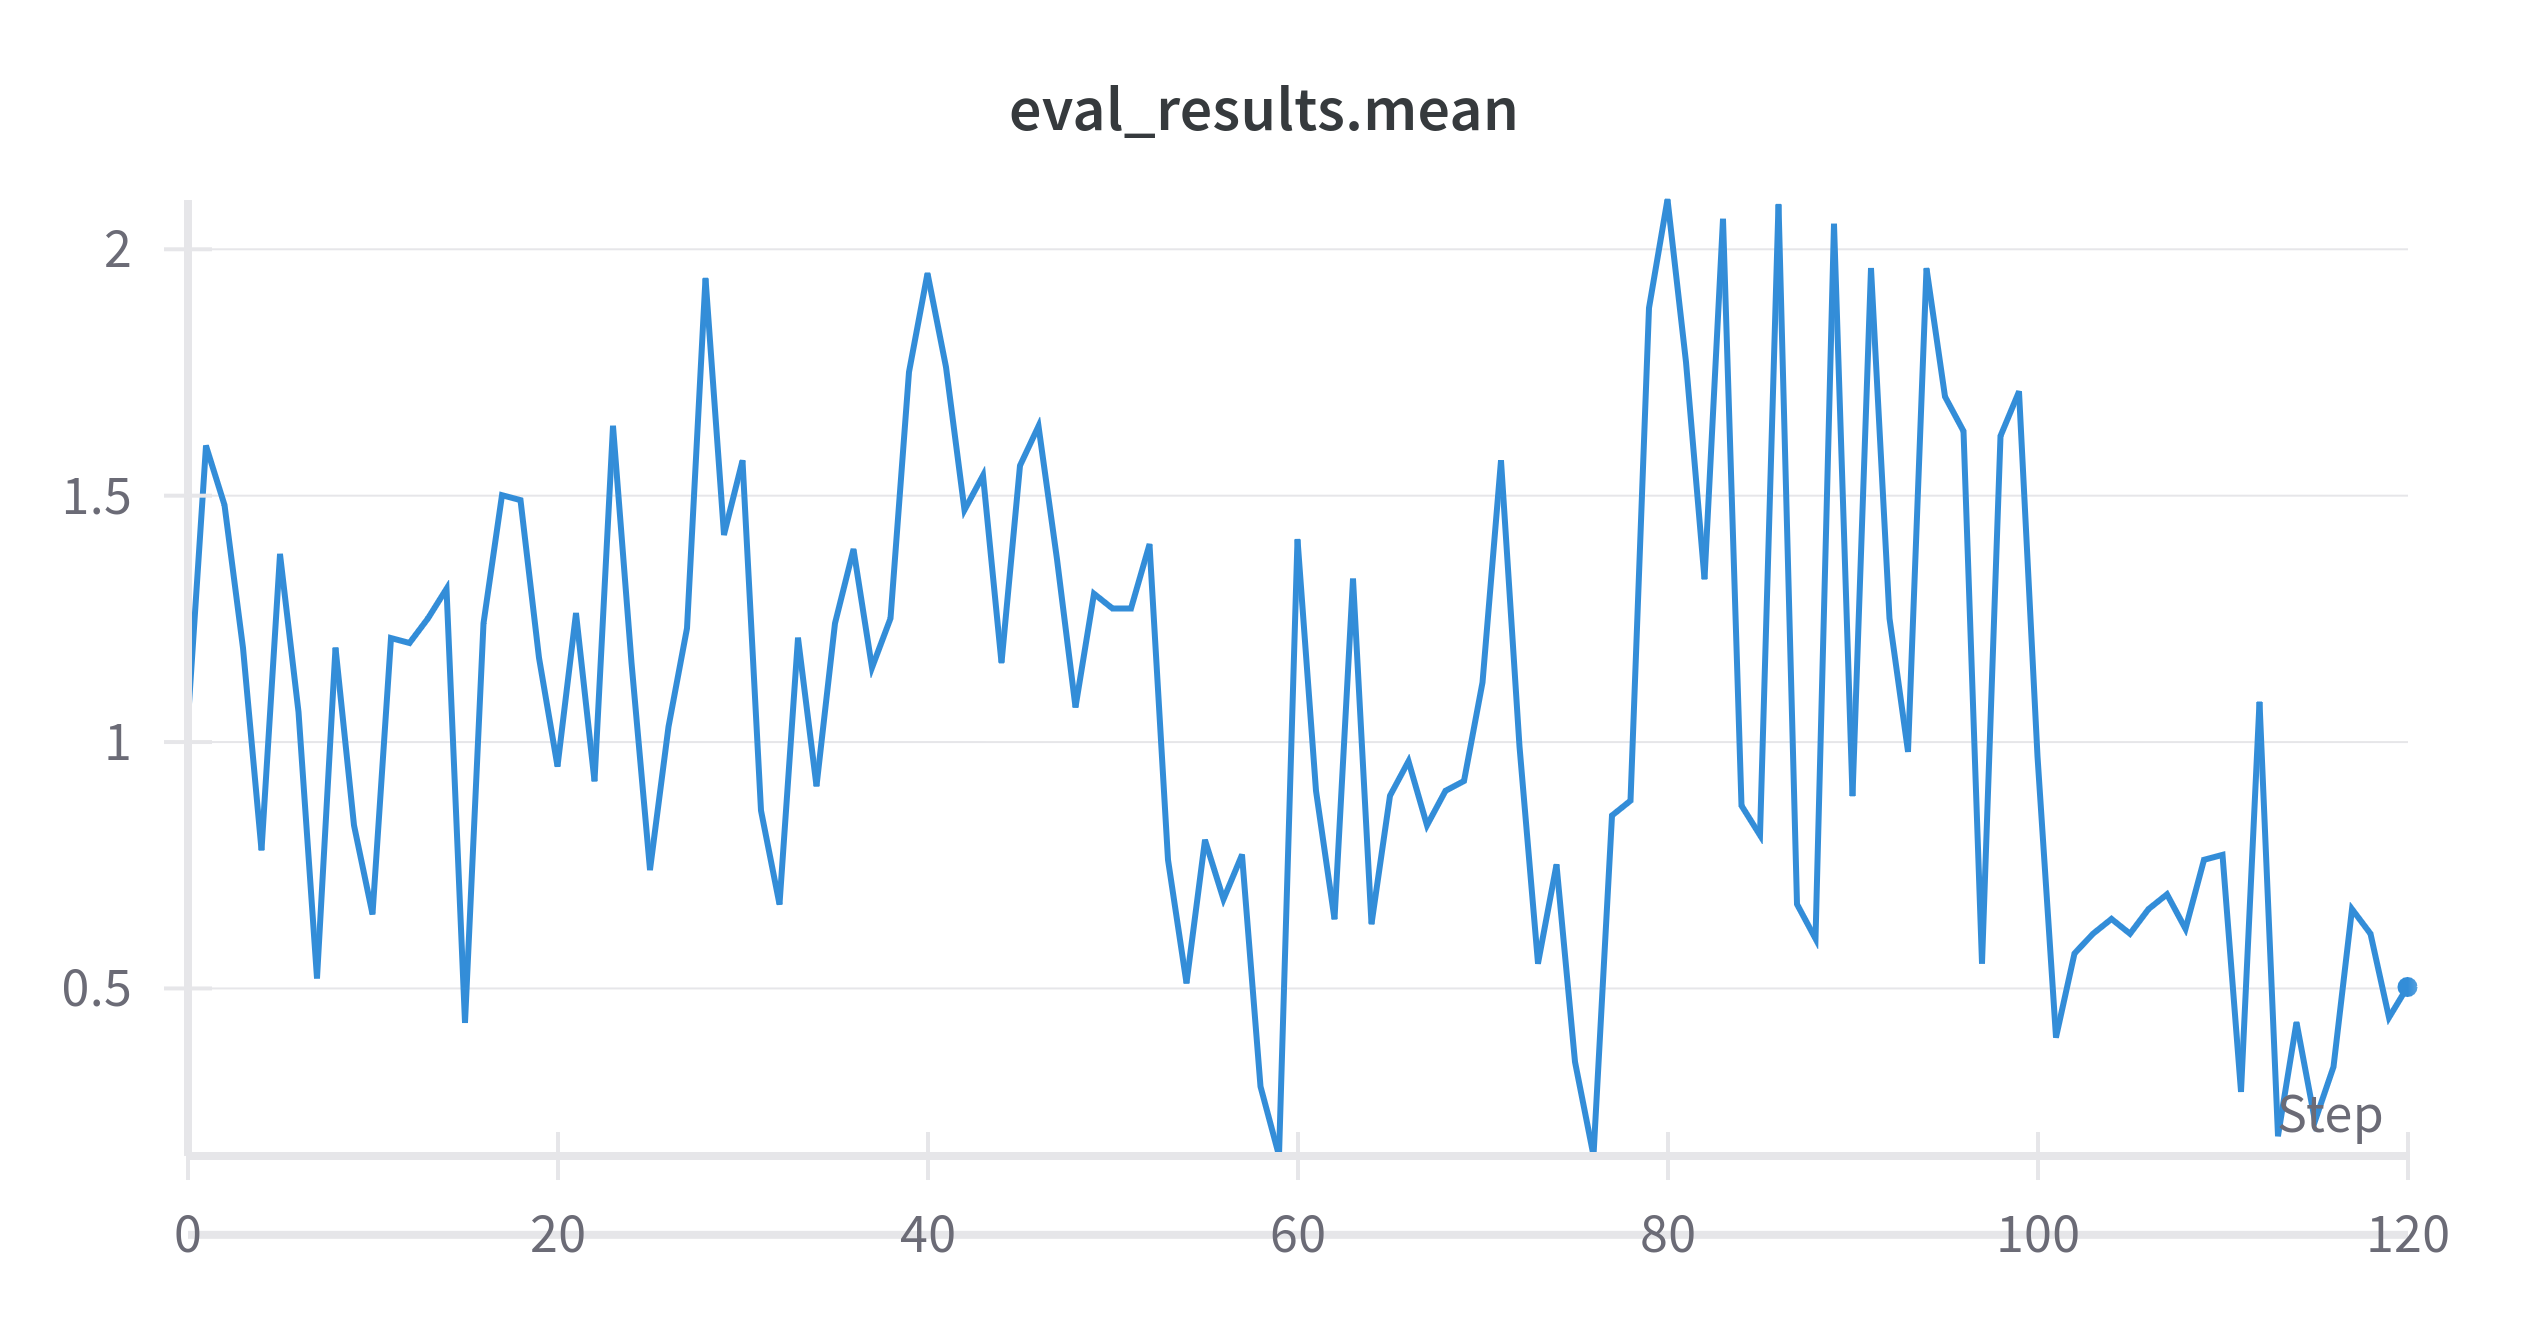
\includegraphics[width=\linewidth]{results/IQL.png}
  \caption{
    Training curve for Simple DQN Agent
  }
  \Description{Training curve for Simple DQN Agent}
  \label{fig:dqn}
\end{figure*}

\begin{figure*}[h]
  \centering
  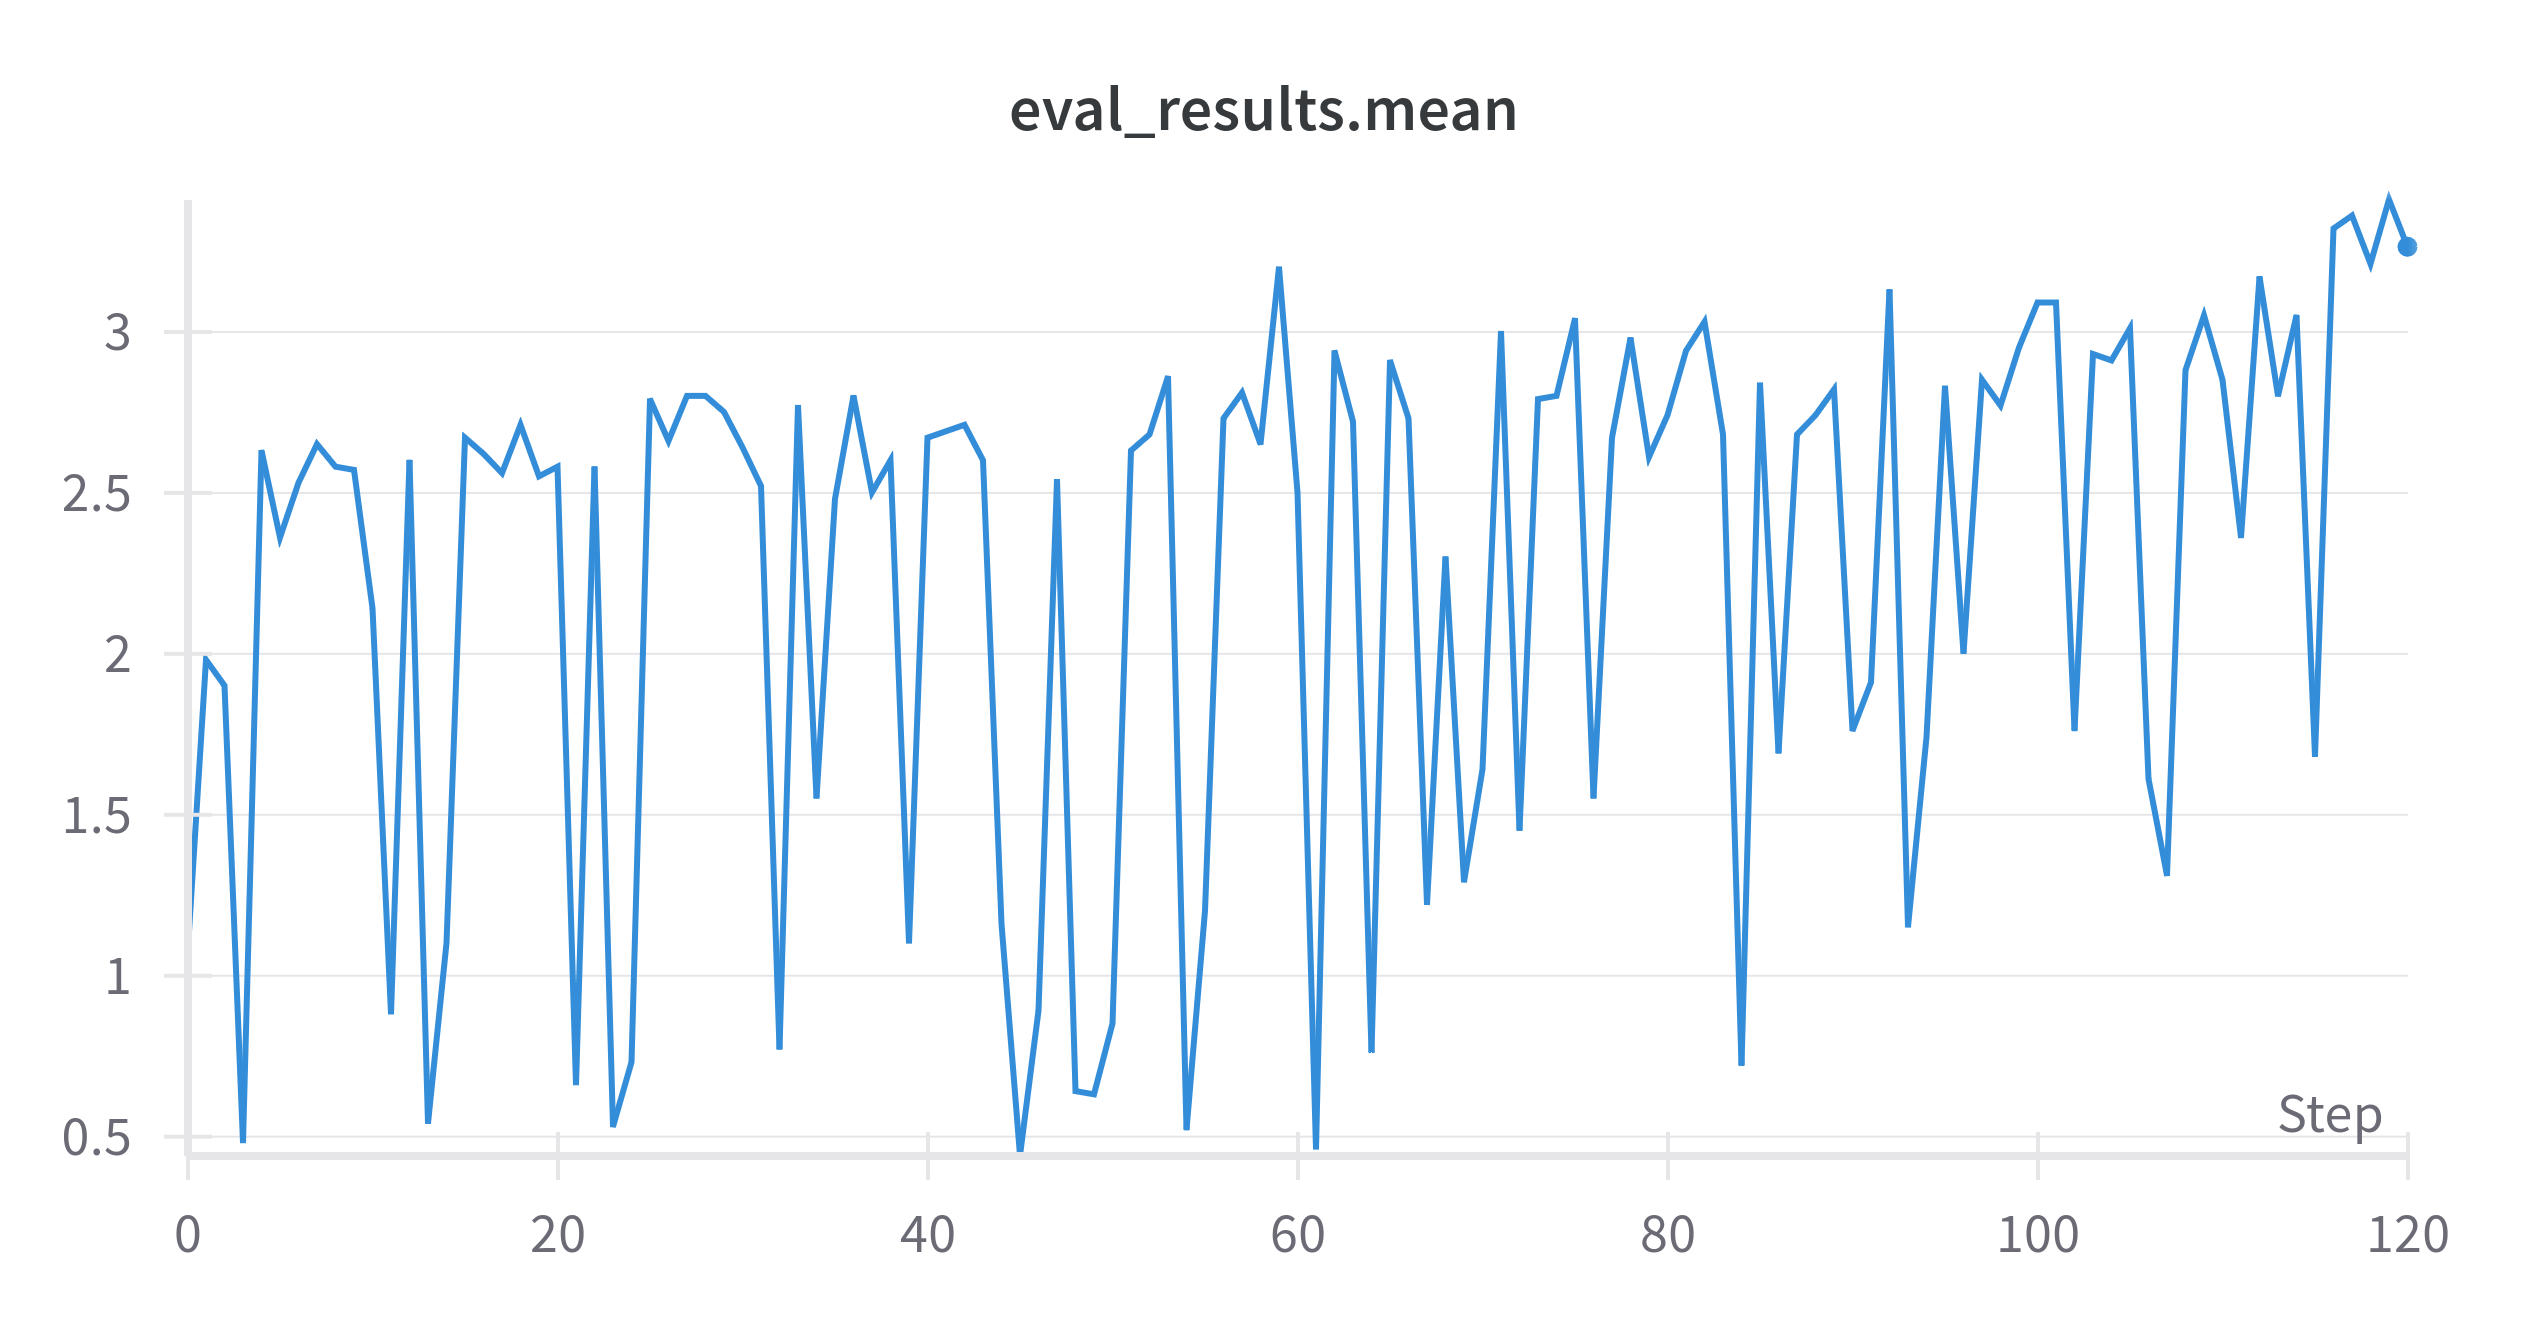
\includegraphics[width=\linewidth]{results/RAINBOW-mean.png}
  \caption{
    Training curve for Rainbow Agent
  }
  \Description{Training curve for Rainbow Agent}
  \label{fig:rainbow}
\end{figure*}

% \begin{figure*}[h]
%   \centering
%   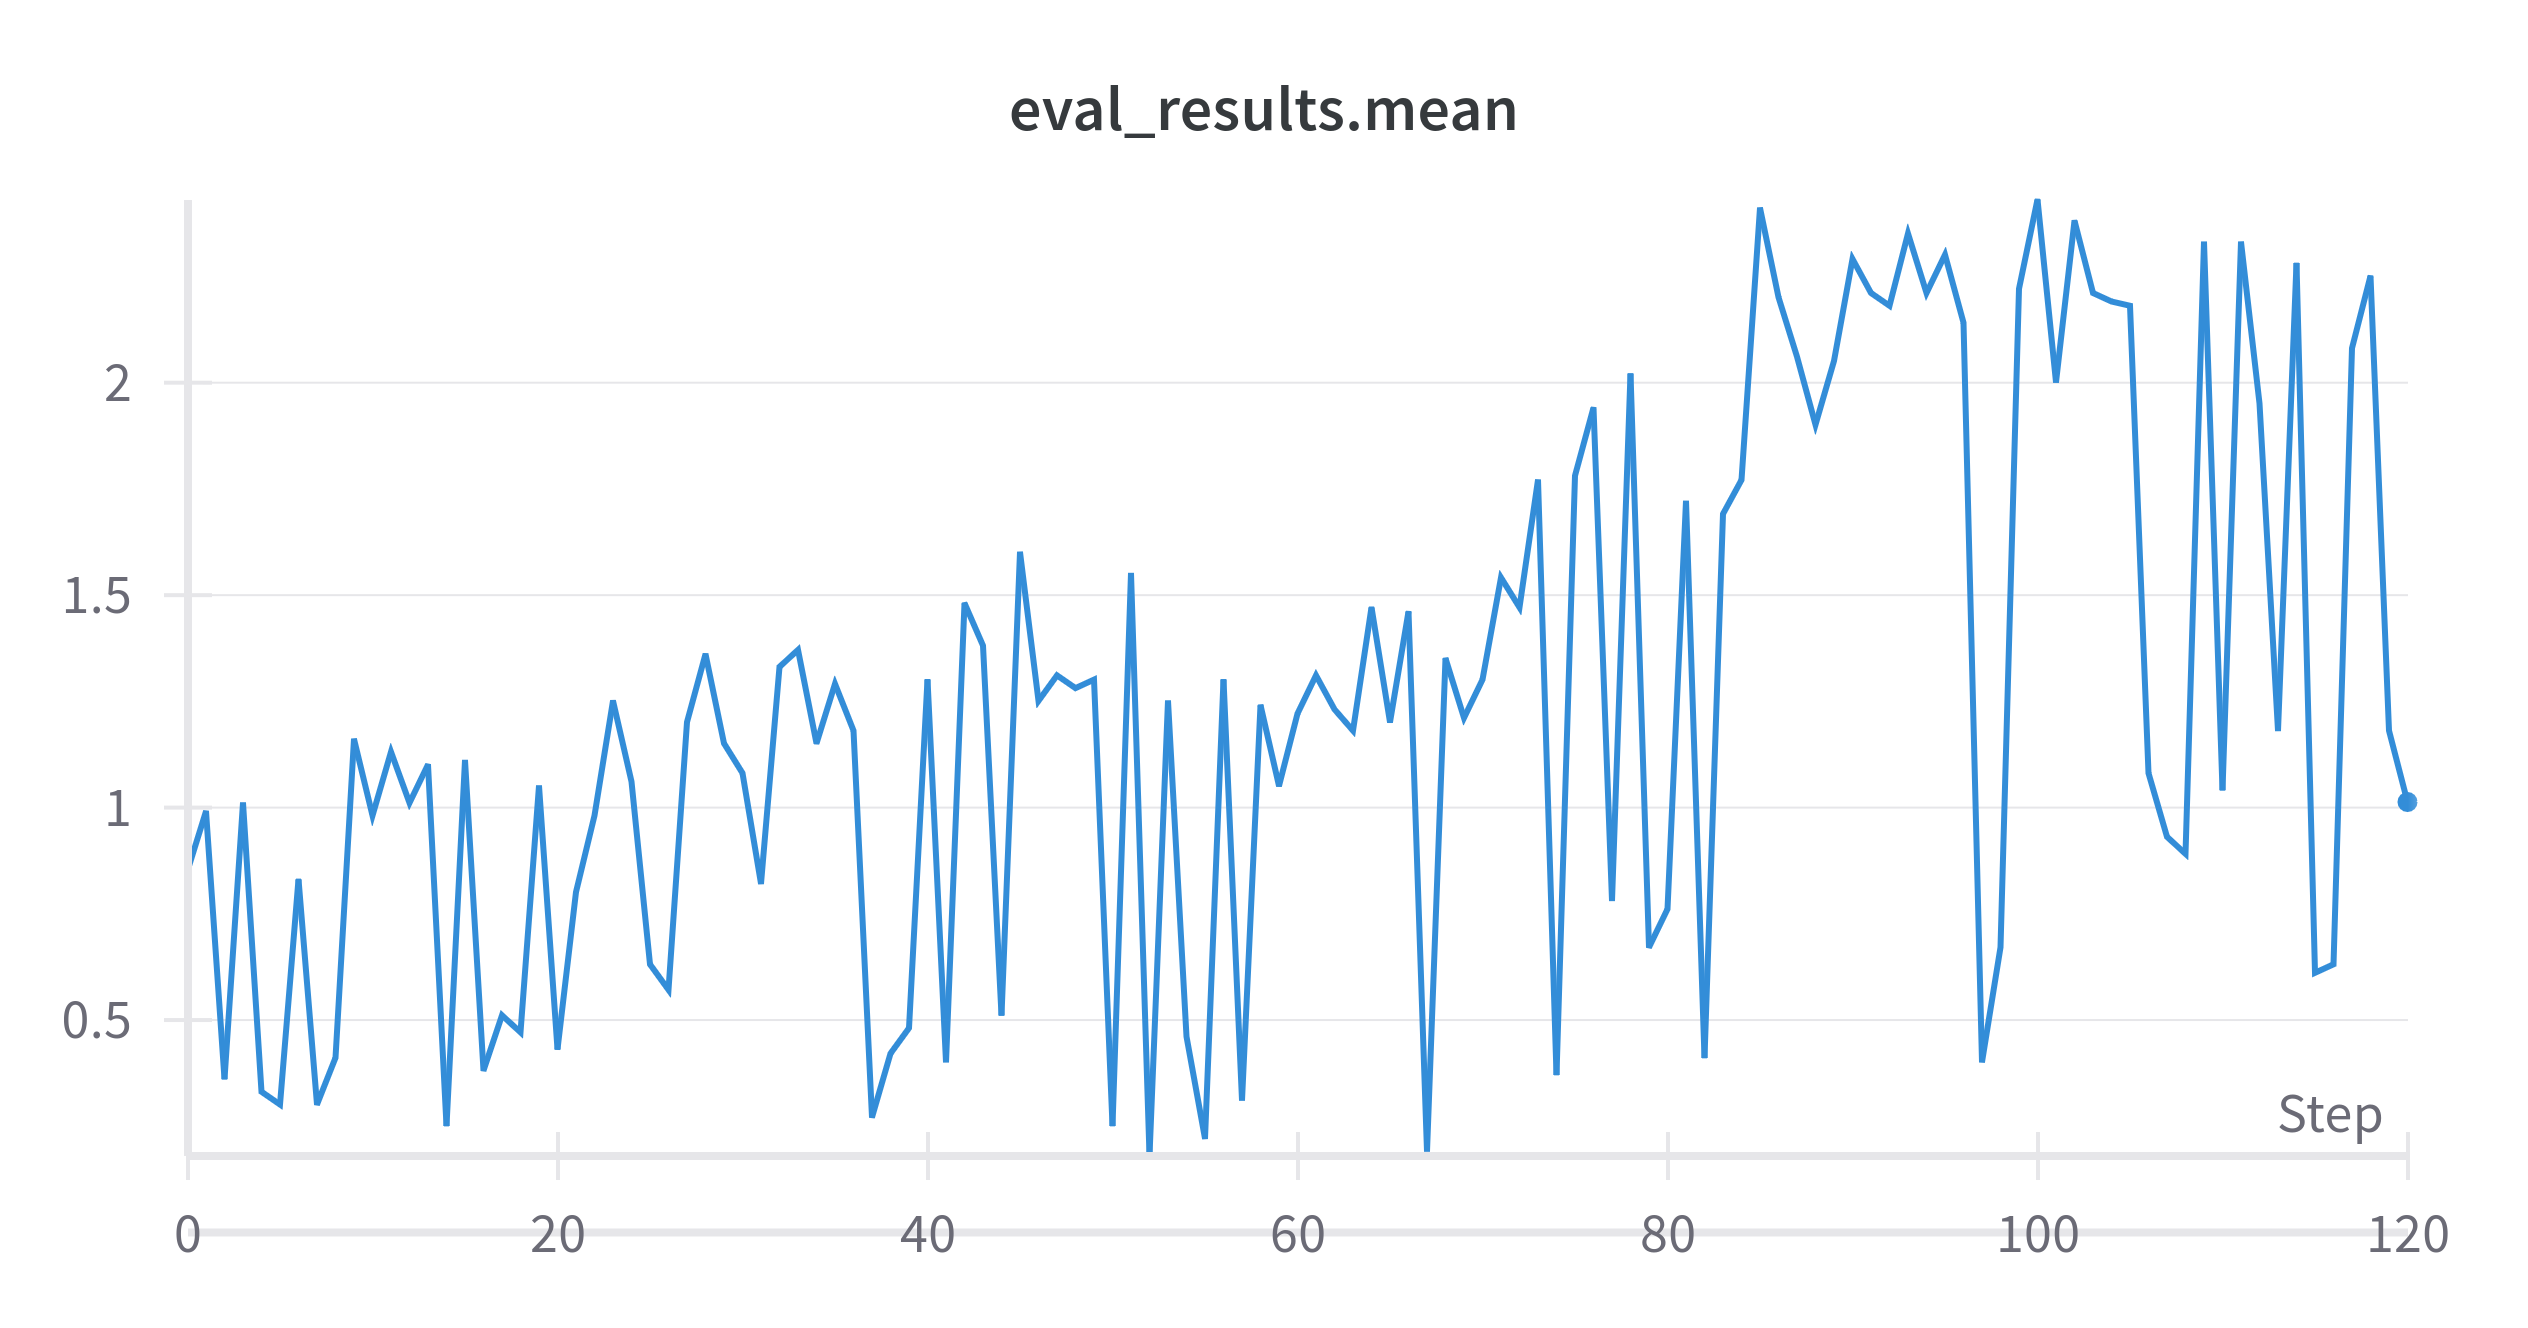
\includegraphics[width=\linewidth]{results/RAINBOW-3-mean.png}
%   \caption{
%     Training curve for Rainbow-3 Agent
%   }
%   \Description{Training curve for Rainbow-3 Agent}
% \end{figure*}

% \begin{figure*}[h]
%   \centering
%   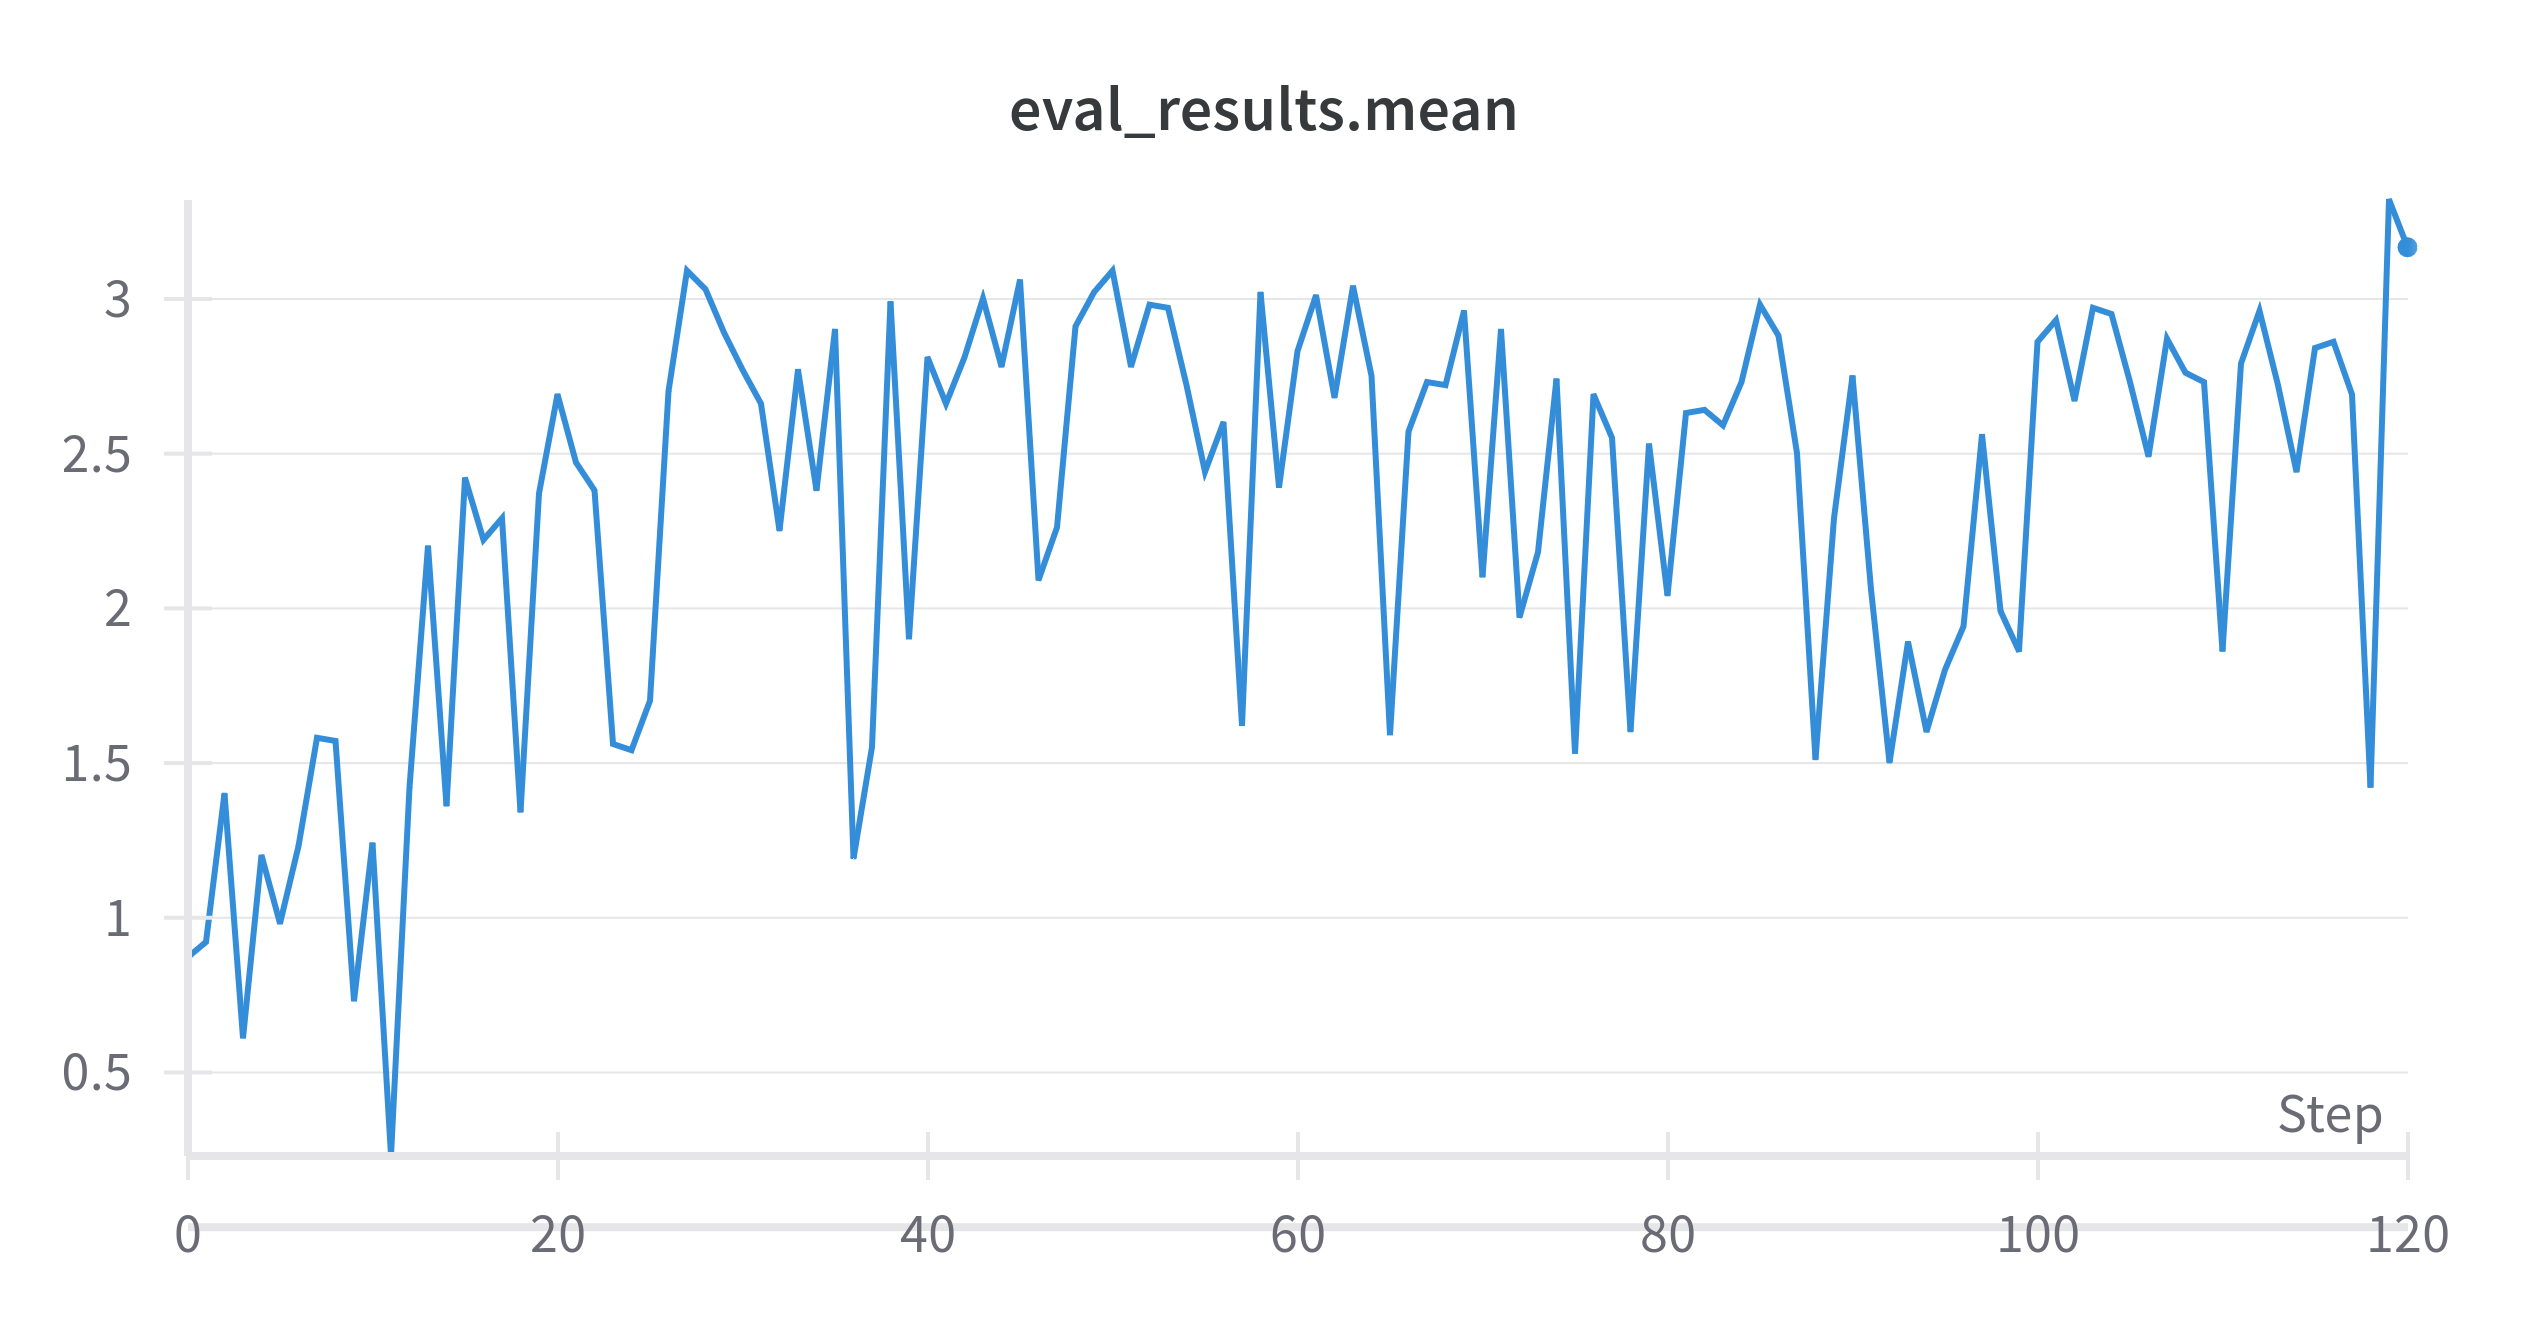
\includegraphics[width=\linewidth]{results/RAINBOW-5-mean.png}
%   \caption{
%     Training curve for Rainbow-5 Agent
%   }
%   \Description{Training curve for Rainbow-5 Agent}
% \end{figure*}


% \begin{figure*}[h]
%   \centering
%   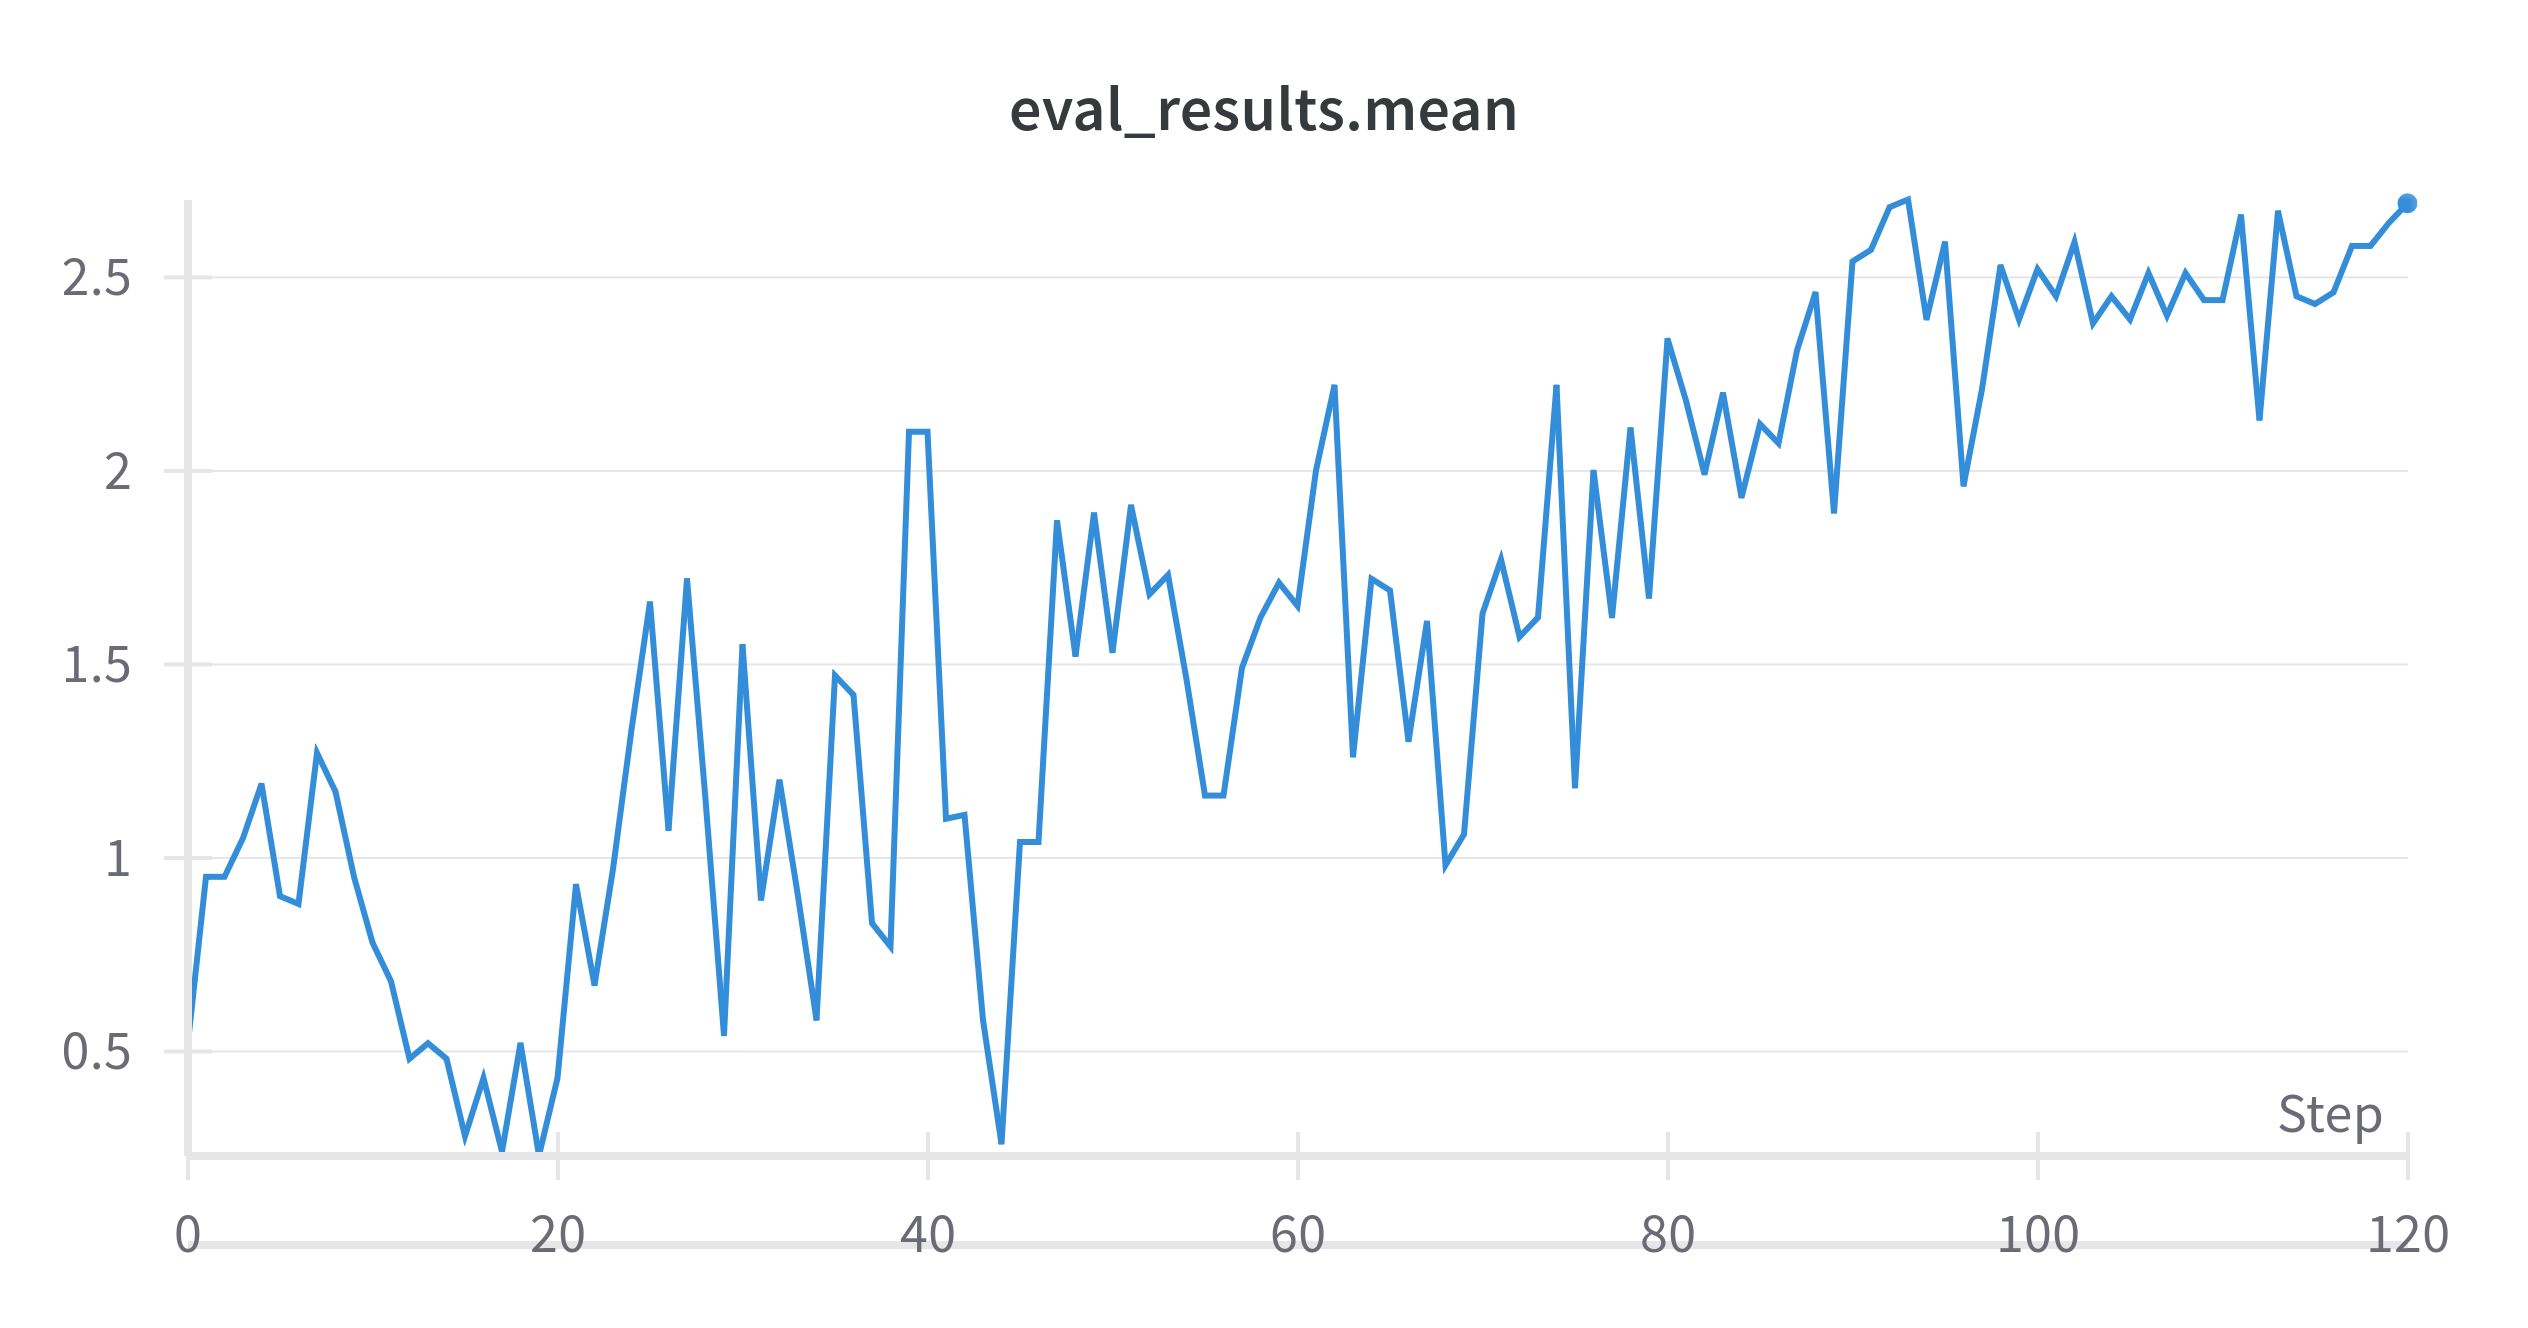
\includegraphics[width=\linewidth]{results/SAD-mean.png}
%   \caption{
%     Training curve for SAD Agent
%   }
%   \Description{Training curve for SAD Agent}
% \end{figure*}

\begin{figure*}[h]
  \centering
  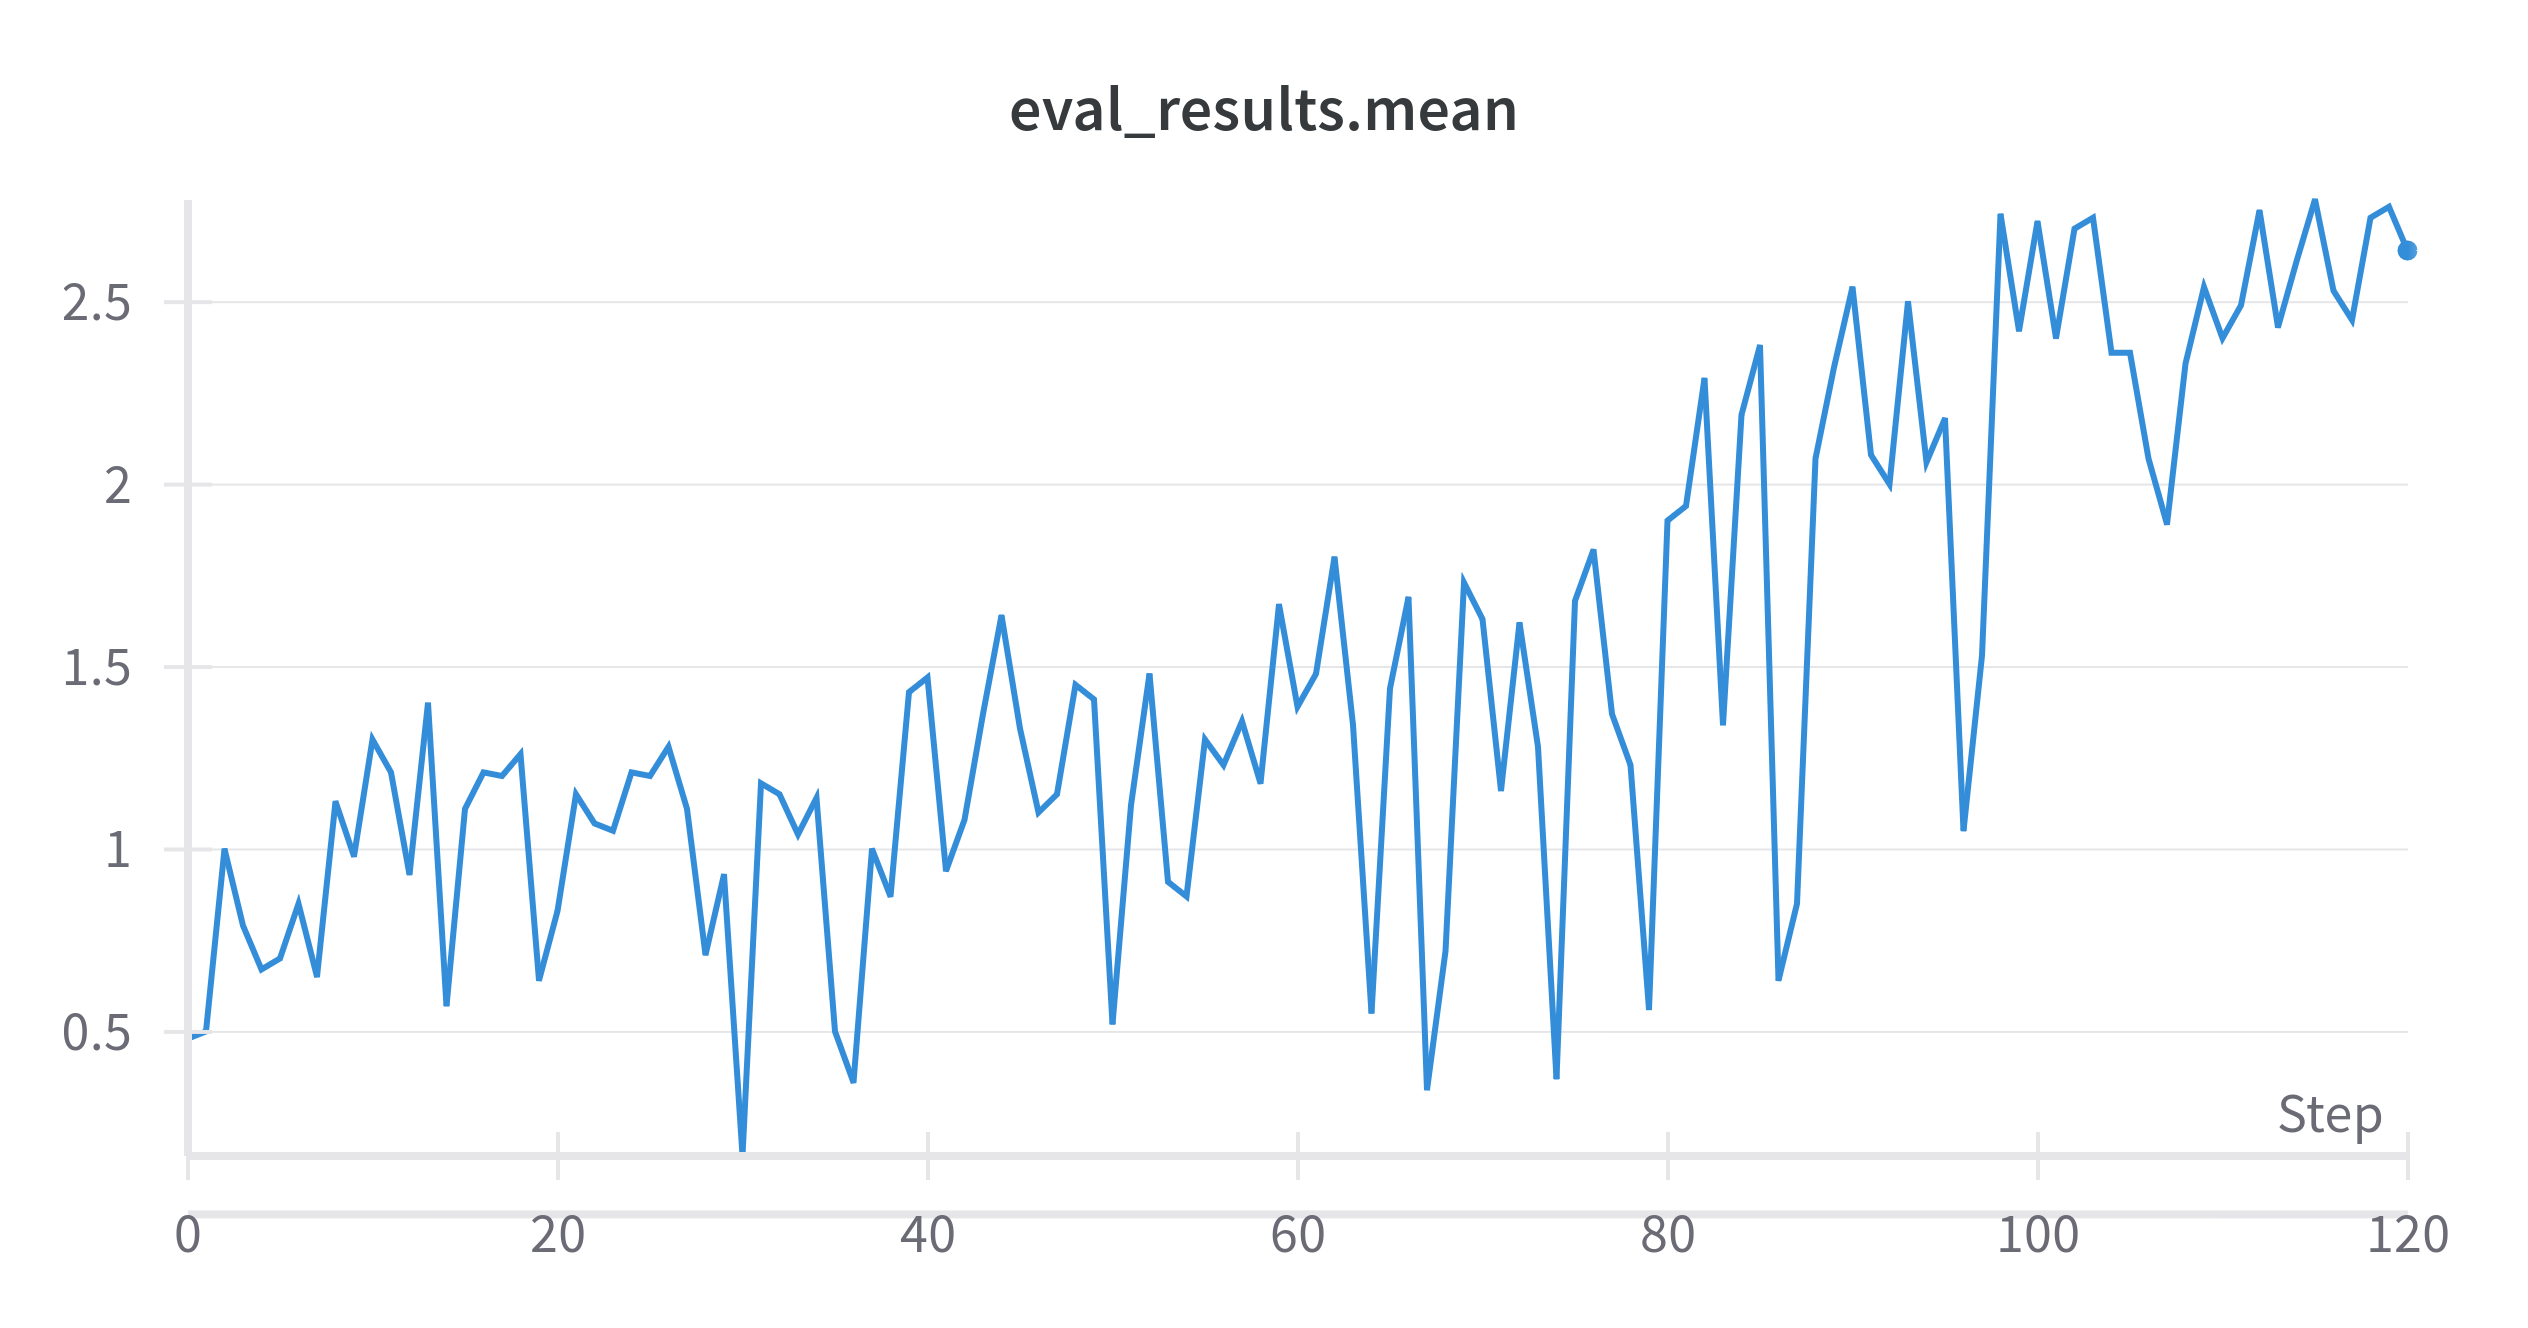
\includegraphics[width=\linewidth]{results/SAD-3-mean.png}
  \caption{
    Training curve for SAD-3 Agent
  }
  \Description{Training curve for SAD-3 Agent}
  \label{fig:sad3}
\end{figure*}
\begin{table*}
    \caption{Performance of learning agents in Cross-Play}
    \label{tab:xp_performance}
    \begin{tabular}{|c|c|c|c|c|c|c|c|c|}
      \toprule
        \textbf{Agent 1$\backslash$2}   &
        \textbf{Simple DQN}  &
        \textbf{Rainbow}     &
        \textbf{Rainbow-3}   &
        \textbf{Rainbow-5}   &
        \textbf{Distributed} &
        \textbf{SAD}         &
        \textbf{SAD-3}       &
        \textbf{Avg XP} \\
      \midrule
      \textbf{Simple DQN} &
        - &
        1.2(0.91) &
        0.78(0.92) &
        1.16(0.8) &
        0.53(0.8) &
        N/A &
        N/A &
        0.92(0.86) \\
      
        \textbf{Rainbow} &
        1.1(0.98) &
        - &
        1.49(1.6) &
        2.5(1.4) &
        1.36(1.36) &
        N/A &
        N/A &
        1.61(1.33) \\

        \textbf{Rainbow-3} &
        0.91(0.95) &
        1.56(1.59) &
        - &
        1.87(1.4) &
        1.07(1.3) &
        N/A &
        N/A &
        1.35(1.31) \\

        \textbf{Rainbow-5} &
        0.96(0.99) &
        2.39(1.43) &
        1.6(1.37) &
        - &
        1.18(1) &
        N/A &
        N/A &
        1.53(1.2) \\

        \textbf{Distributed} &
        1.25(1.02) &
        1.61(1.40) &
        1.26(1.31) &
        1.28(1.01) &
        - &
        N/A &
        N/A &
        1.35(1.19) \\

        \textbf{SAD} &
        N/A                  &
                N/A                  &
                N/A                  &
                N/A                  &
                N/A                  &
                -                    &
                2.4(1)               &
                2.4(1)
                \\ 



        \textbf{SAD-3}       &
        N/A                  &
        N/A                  &
        N/A                  &
        N/A                  &
        N/A                  &
        2.11(0.8)            &
        -                    &
        2.11(0.8)
        \\ 

        \textbf{Avg XP}      &
        1.01(0.99)           &
        1.69(1.33)           &
        1.28(1.3)            &
        1.7(1.15)            &
        1.04(1.12)           &
        2.11(0.8)            &
        2.4(1)               &
        \\ 
    \bottomrule
  \end{tabular}
  \end{table*}

\subsection*{Self-Play Performance}


Table~\ref{tab:sp_performance} shows the performance of the learning agents in the two-player self-play version of Hanabi. The agents are evaluated based on their ability to achieve a high score in the game. The final score is an average of the score achieved over 1000 episodes. The standard deviation of the final score is also included to show the stability of the learning process. See Appendix ~\ref{app:full_results} for the full results.

It is important to note that the rule-based approaches generally outperform the learning agents when considering sample-limited training, with only large-scale RL frameworks like R2D2+SAD \cite{huSimplifiedActionDecoder2021} and ACHA \cite{bardHanabiChallengeNew2020a} outperforming rule-based approaches.

We observe that none of the agents could achieve an average high score in the game. While not a focus of this study, we can attribute this to the sample's limited training setting and the higher complexity of the small version compared to the full game. 

The simple Dueling Double DQN fails to learn the game effectively and struggles to learn an optimal policy for the game. With a score of 0.502, we can conclude that the agent cannot play 1 card correctly on average. It is important to note that, at best, the agent can reach a score of 2.19 earlier in the training process, which shows some promise in the agent's ability to learn the game. However, the agent fails to maintain this performance and quickly regresses to a lower score. Without a clear trend in performance, we can conclude that the agent cannot effectively learn a policy for the game. This can be observed in Figure ~\ref{fig:dqn}.

The Rainbow DQN shows an impressive improvement in performance over the simple DQN agent, and we can identify a general improvement over time in its performance. However, we observe a cycle of regression and correction in the training, which we will discuss later.

When using a 1 step history, the Rainbow agent quickly learns a policy but then struggles to improve over time, likely due to the agent learning a suboptimal policy early in the game that it cannot recover from.

When using a 3 step history, we can identify an almost linear improvement in performance over time, with the agent quickly learning a policy and then steadily improving its performance. It performs slightly worse on average than the 1 step history but with a more stable learning curve. This is likely due to more samples being needed when looking at a longer history, which is a limitation of the sample-limited training setting. The final score of the agent is lower due to the aforementioned exploration regression cycle, but with more training, the agent would likely be able to achieve a higher score.

With a 5-step history, the results are similar to the 1-step history, with the agent quickly learning a policy but then struggling to improve over time. The agent receives a slightly lower score than the 1-step history, but due to the sample requirements of the longer history, the agent is likely to perform better with more training.

We compare these Rainbow results with a baseline Rainbow Agent with $\epsilon$-greedy exploration instead of Noisy Networks to evaluate the value of Noisy Network exploration. We find that the Noisy Network exploration is more sample efficient than $\epsilon$-greedy exploration, and the Rainbow agent can quickly achieve a significantly higher score without too much impact on the standard deviation. This is likely due to the Noisy Network exploration being more effective at exploring the state space of the game, and the agent can learn a more effective policy more quickly. However, we observe a cycle of regression and correction, observed in Figure ~\ref{fig:rainbow}, in the noisy network exploration agent. This is likely due to the agent learning a suboptimal policy and correcting itself in a cycle. This is a limitation of the exploration function of the agent, and the agent would likely be able to achieve a higher score and more stable learning curve with more training.

The simplified action decoder shows more stable learning and slightly lower performance than the Rainbow DQN agent. However, it showcases a nearly linear improvement in performance over time with a stable and consistent learning curve. When looking at a 3-step history, observed in Figure ~\ref{fig:sad3}, this improvement is more pronounced. SAD, however, slightly decreases the performance of the agent when compared to the baseline Rainbow DQN agent. This is likely due to the additional information provided to the agent during training, which increases the complexity of the learning process.

The stable training curve and lower standard deviation in the final score outline the value of the SAD algorithm in learning the partnership dynamics of the game more effectively. The SAD algorithm can model the other policy effectively and learn more efficiently from it. This is important as in a game like Hanabi, the partnership dynamics are crucial to achieving a high score.

In the literature, the SAD algorithm has been shown to outperform the Rainbow DQN algorithm in the two-player self-play version of Hanabi \cite{huSimplifiedActionDecoder2021}. However, in this study, the Rainbow DQN algorithm can outperform the SAD algorithm. In the literature, the SAD algorithm is often trained in an unlimited sample setting, with a combination of distributed reinforcement learning and recurrent experience replay. This is likely the reason for the discrepancy in performance between the two algorithms. The SAD algorithm is likely to perform better with more training but, in a sample-limited setting, is less effective than the Rainbow DQN algorithm.

\subsection*{AD-Hoc Teamplay Performance}

Table ~\ref{tab:xp_performance} shows the performance of learning agents in the AD-Hoc Teamplay setting.

By observing the decrease in the average score (Avg XP) and increase in the standard deviation of the final score, we find that all the agents struggle to cooperate effectively in cross-play (XP) settings, except for the simple DQN, which seems to improve, which can be attributed to the skill of its partners. The general decrease in the score and increase in the standard deviation is likely due to the agents learning arbitrary conventions that are specific to their partners during training, or "idiosyncratic conventions" as described by \textcite{lucasAnyPlayIntrinsicAugmentation2022}. This is a significant limitation of the current state-of-the-art in Hanabi, and it raises the importance of finding sample-efficient algorithms for Hanabi that can generalize to new partners.


\section{Conclusions and Future Work}
\label{sec:conclusion}
This work presented an evaluation of the impact of Deep-Q-Learning techniques on a smaller version of the Hanabi Challenge. We have shown that the Rainbow DQN algorithm improves the sample efficiency of the agents over the simple DQN algorithm. We have also shown that the Simplified Action Decoder (SAD) algorithm significantly stabilizes the self-play learning process, at a slight cost to performance. We have also outlined the value of efficient exploration on sample efficiency with Noisy Networks as an exploration strategy over $\epsilon$-greedy.

While both techniques showcase promising results in the self-play setting, the agents struggle to cooperate effectively in the AD-Hoc Teamplay setting. This highlights the importance of developing sample-efficient algorithms that can generalize to new partners effectively.

These results are limited by the computational cost of training Hanabi agents and the sample-limited setting of the experiments. Future work can extend these experiments by training a larger population of diverse agents to better showcase the performance capabilities of the agents. Additionally, the impact of hierarchical reinforcement learning \cite{vezhnevetsFeUdalNetworksHierarchical2017} on the performance of agents in Hanabi can be explored to help agents learn to navigate the action space more effectively by breaking it down into smaller sub-tasks, with frameworks like Option-Critic architecture \cite{baconOptionCriticArchitecture2016}. Techniques like Meta-Reinforcement \cite{beckSurveyMetaReinforcementLearning2024} Learning can pave the way for more adaptable agents, and more research in the direction of Few-Shot coordination \cite{nekoeiFewshotCoordinationRevisiting2023} can help agents learn to cooperate effectively with new partners with limited exposure.


\printbibliography

\appendix
\section{Extended Results and Discussion}
\label{app:full_results}
This section provides a full overview of the training and evaluation results of the agents in the two-player self-play setting. The training and evaluation results are presented in the form of the average score and loss curves for each agent during training. The training and loss curves provide insights into the learning process of the agents and their performance in the game and are presented in Figures ~\ref{fig:dqnmean} - ~\ref{fig:sad3loss}.

We observe that the simple DQN agent struggles to learn the game effectively and fails to achieve a high score in the game. The agent's performance is unstable, and it fails to maintain a high score over time, despite the loss curve showing a decreasing trend. The agent's performance is likely limited by the simple DQN architecture and the sample-limited training setting. The agent's performance is presented in Figures ~\ref{fig:dqnmean} and ~\ref{fig:dqnloss}.

All of the Rainbow agents show the highest performance in the game, with the base Rainbow agent achieving the highest average score. The Rainbow agents show a cyclic pattern of improvement and regression in their performance, discussed earlier in Section ~\ref{sec:results}. Interestingly, the Rainbow agents with a 3-step and 5-step history show no clear trend in their loss curves, despite showing a general improvement in their performance over time. This is only present in the Rainbow agents, and it is likely due to the added noise from the Noisy Networks exploration strategy in combination with the larger history lengths causing some instability in the learning process. It is also likely linked to the cyclic pattern of improvement and regression in the Rainbow agents' performance. The Rainbow agents' performance is presented in Figures ~\ref{fig:rainbowmean} - ~\ref{fig:rainbow5loss}.

Both the SAD and Distributed agents show a very pronounced rapid increase in loss for the first 10-20 episodes, followed by a rapid decrease in loss. This can likely be explained by the lack of meaningful experiences in the replay buffer at the start of training, leading to a high TD error and thus a high loss. As the agents gain more experience, the loss decreases rapidly, indicating that the agents are learning effectively from the experiences. Additionally, the target network would only begin to stabilize after a few episodes, leading to a decrease in the loss. This is also likely exacerbated by the initial fully random exploration coupled with Hanabi's partially observable nature. The SAD and Distributed agents' performance is presented in Figures ~\ref{fig:distributed} - ~\ref{fig:sad3loss}.

\begin{figure*}[h]
    \centering
    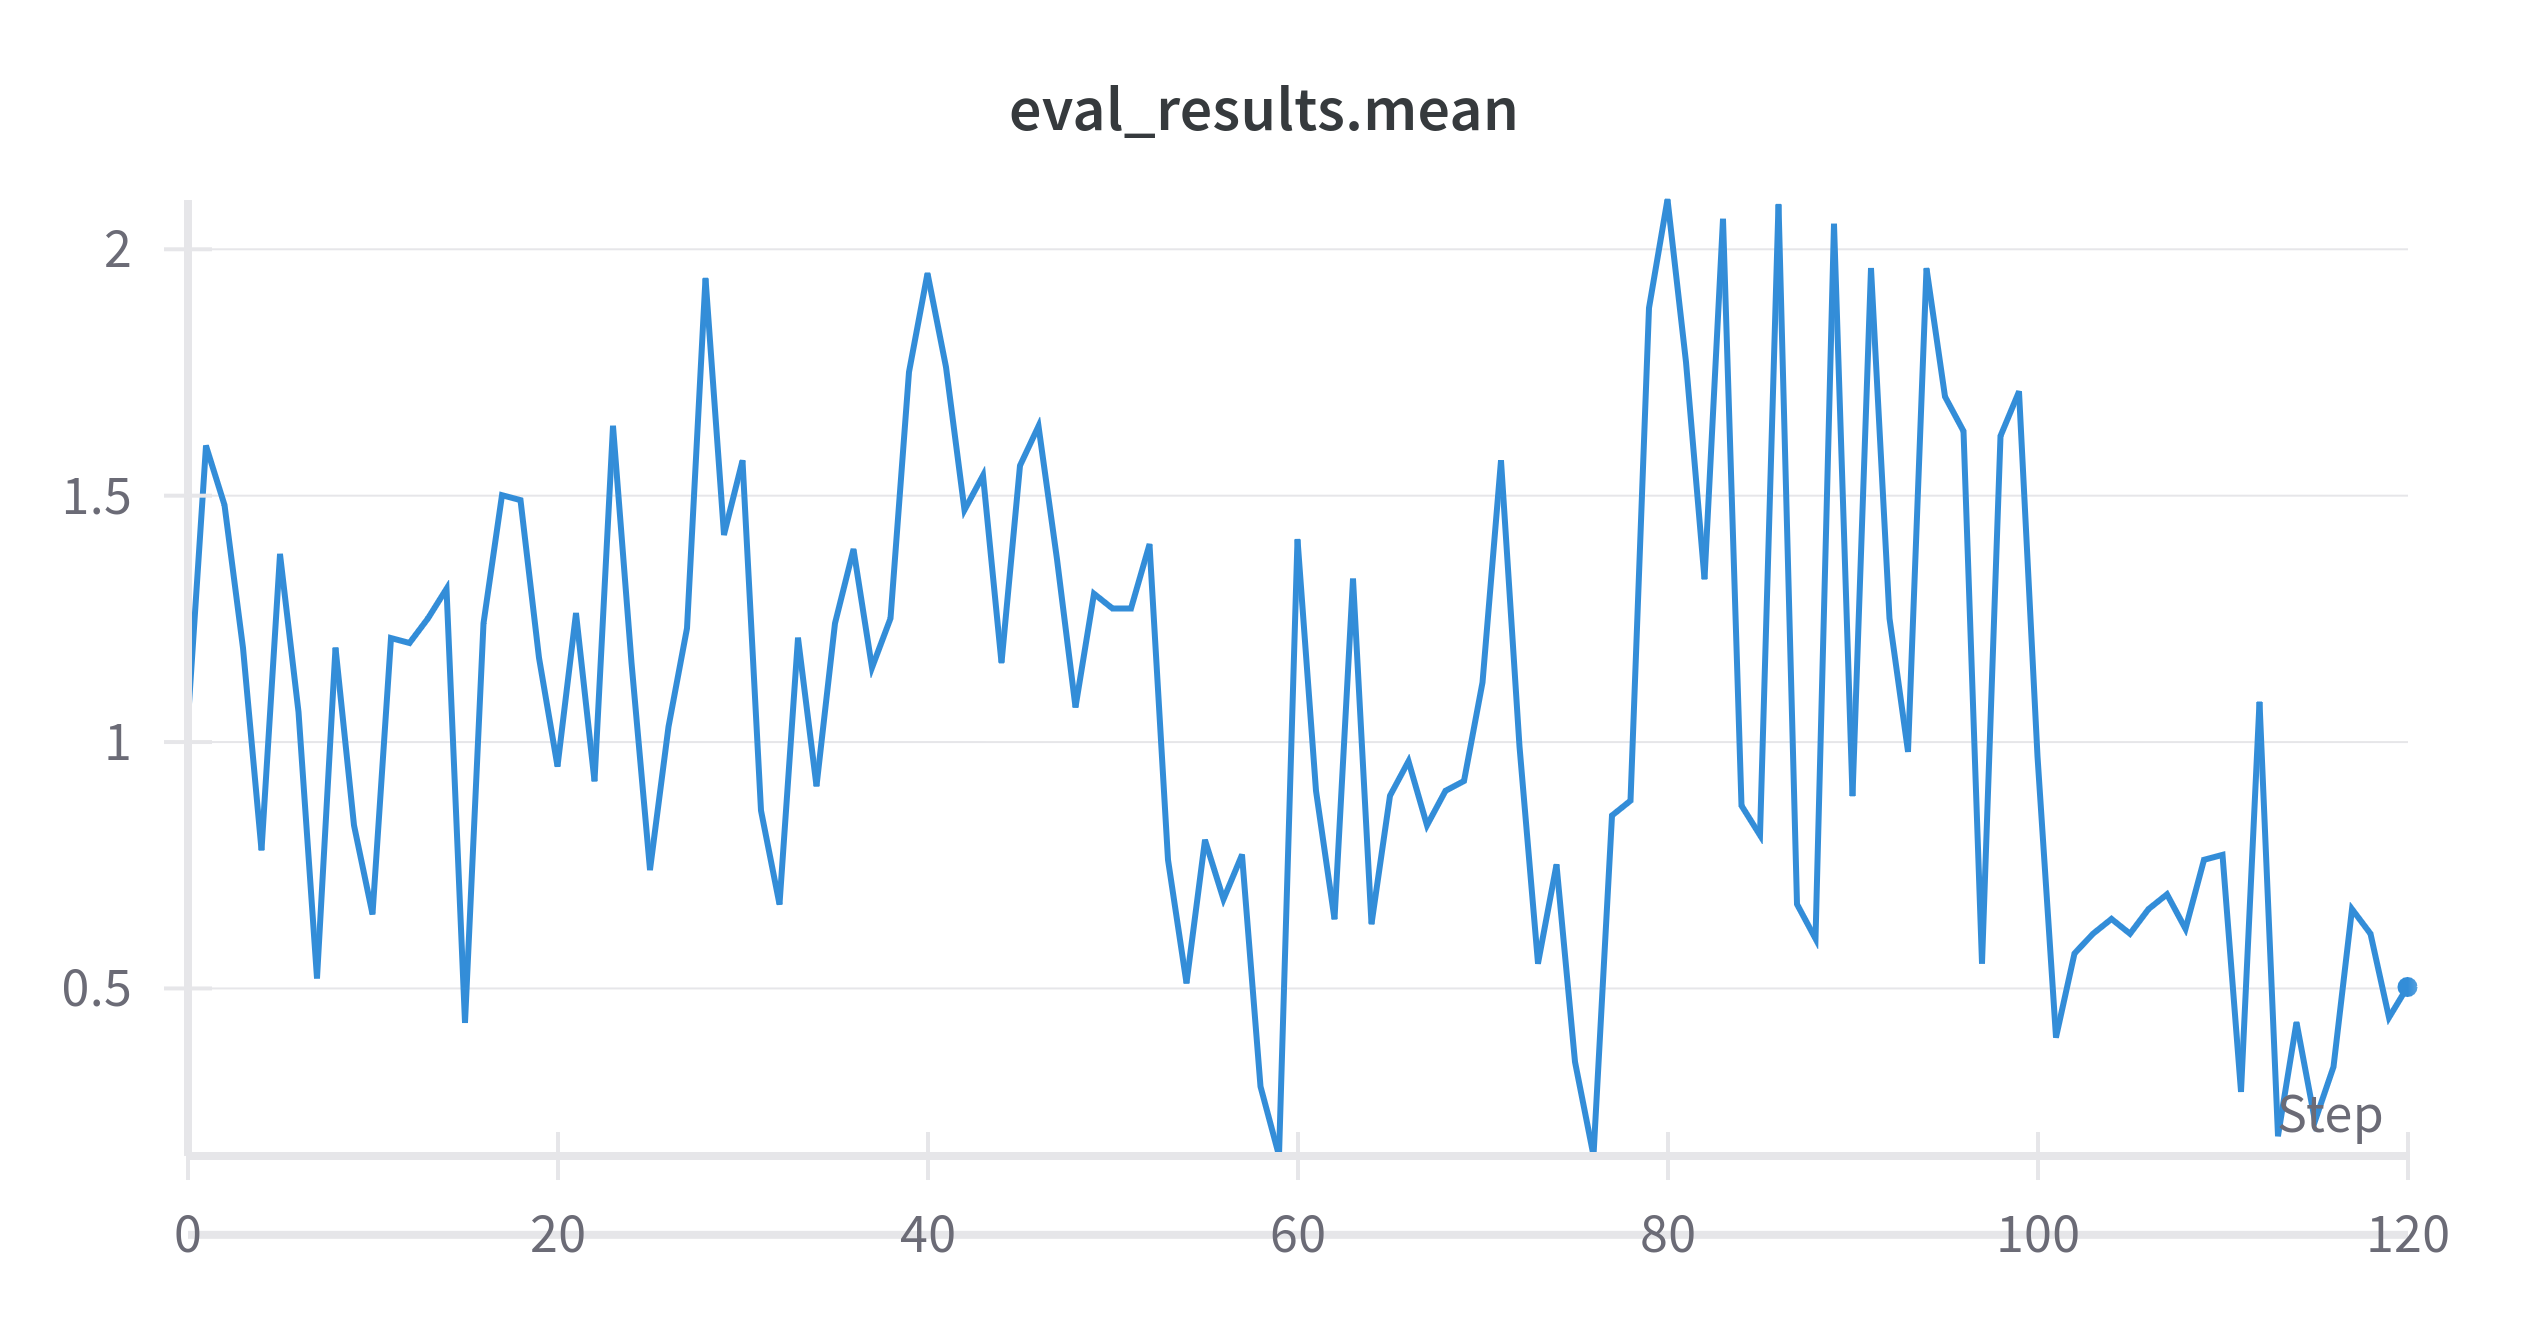
\includegraphics[width=\linewidth]{results/IQL.png}
    \caption{
      Training curve for Simple DQN Agent
    }
    \Description{Training curve for Simple DQN Agent}
    \label{fig:dqnmean}
  \end{figure*}
  
  \begin{figure*}[h]
    \centering
    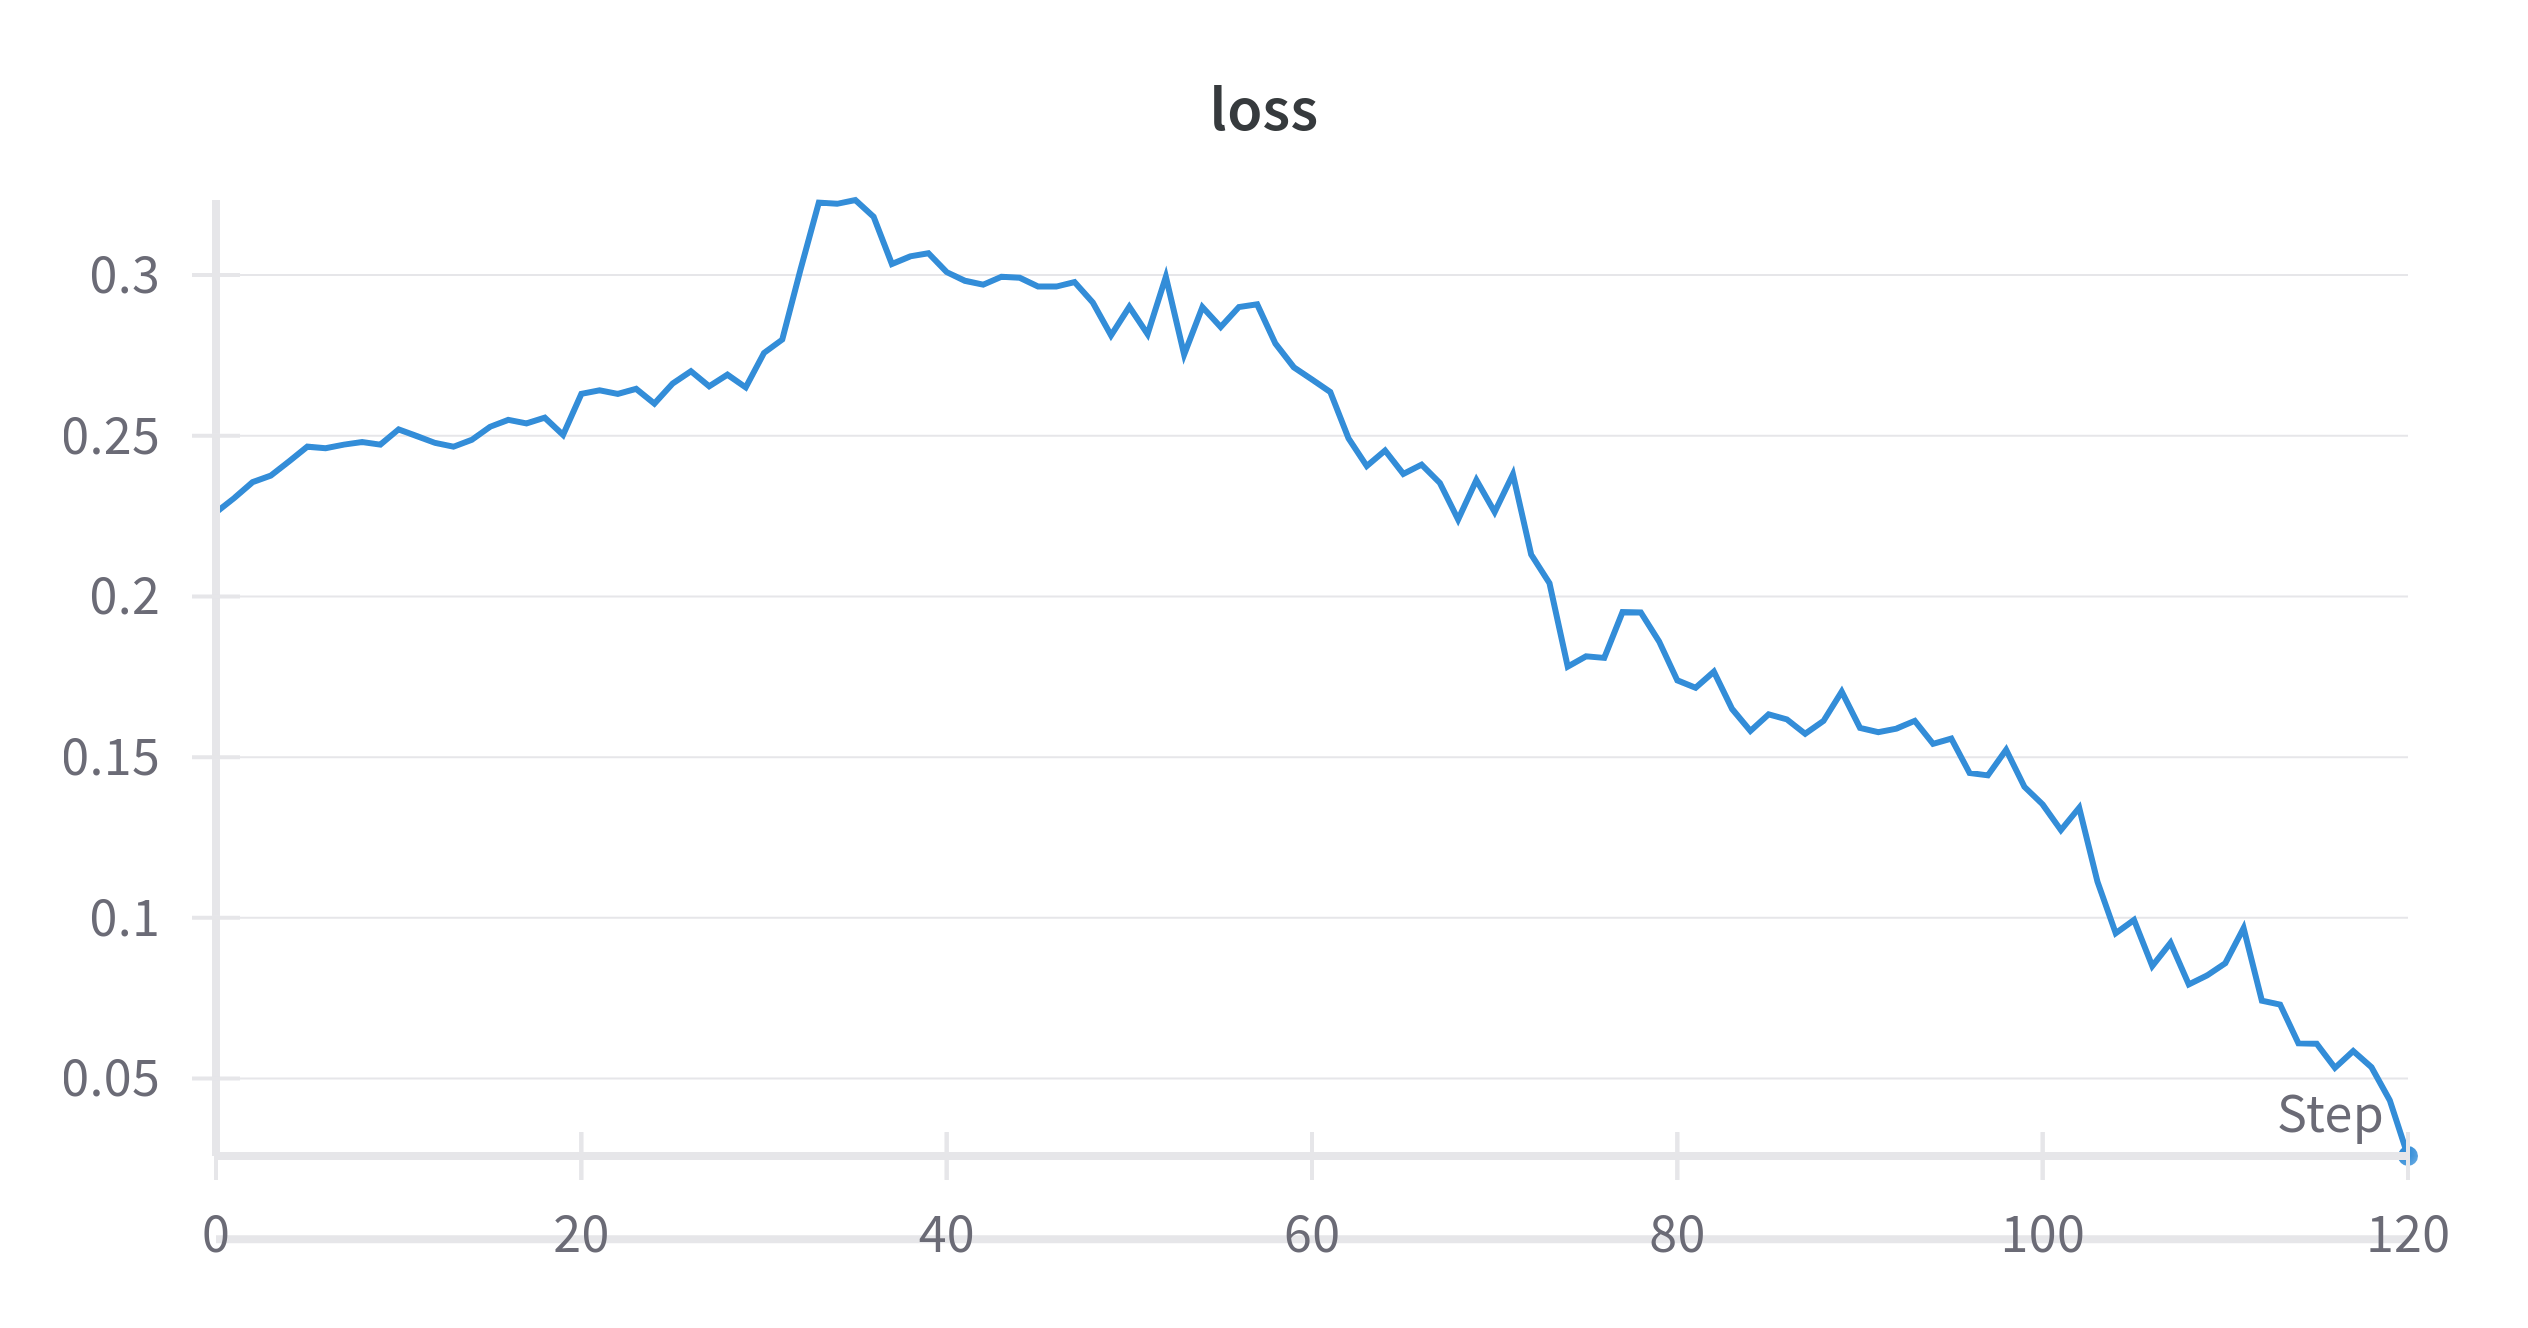
\includegraphics[width=\linewidth]{results/IQL-loss.png}
    \caption{
        Loss curve for Simple DQN Agent
    }
    \Description{Loss curve for Simple DQN Agent}
    \label{fig:dqnloss}
  \end{figure*}



  \begin{figure*}[h]
    \centering
    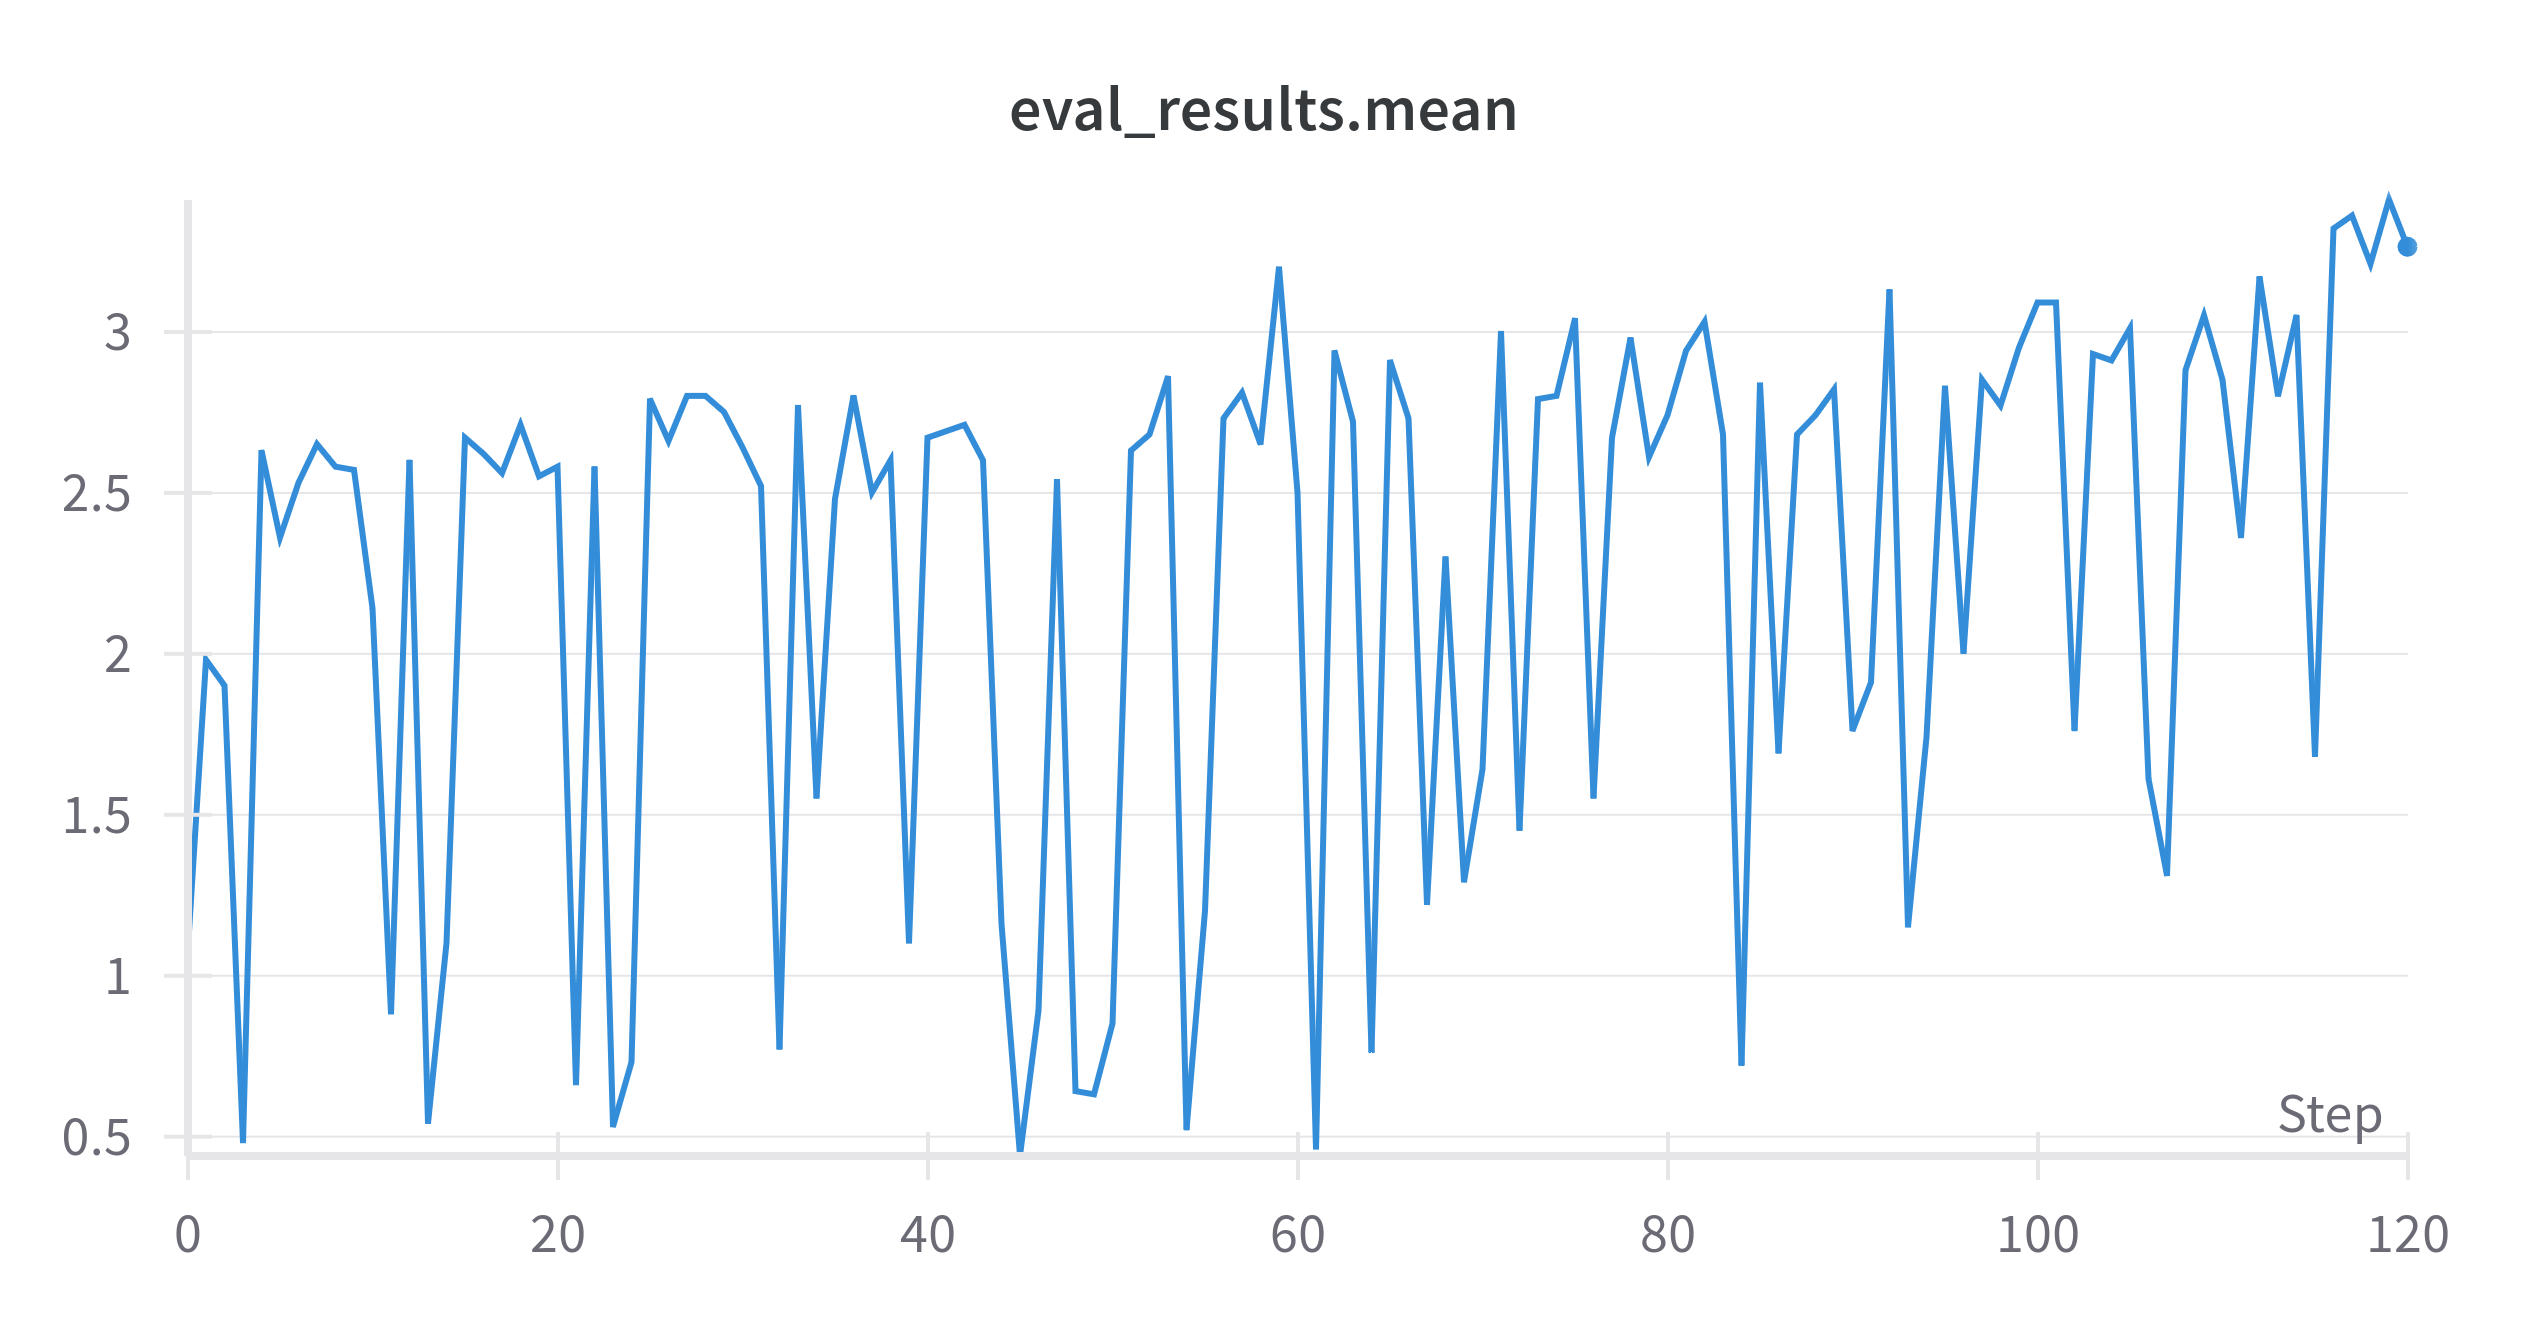
\includegraphics[width=\linewidth]{results/RAINBOW-mean.png}
    \caption{
      Training curve for Rainbow Agent
    }
    \Description{Training curve for Rainbow Agent}
    \label{fig:rainbowmean}
  \end{figure*}
  \begin{figure*}[h]
    \centering
    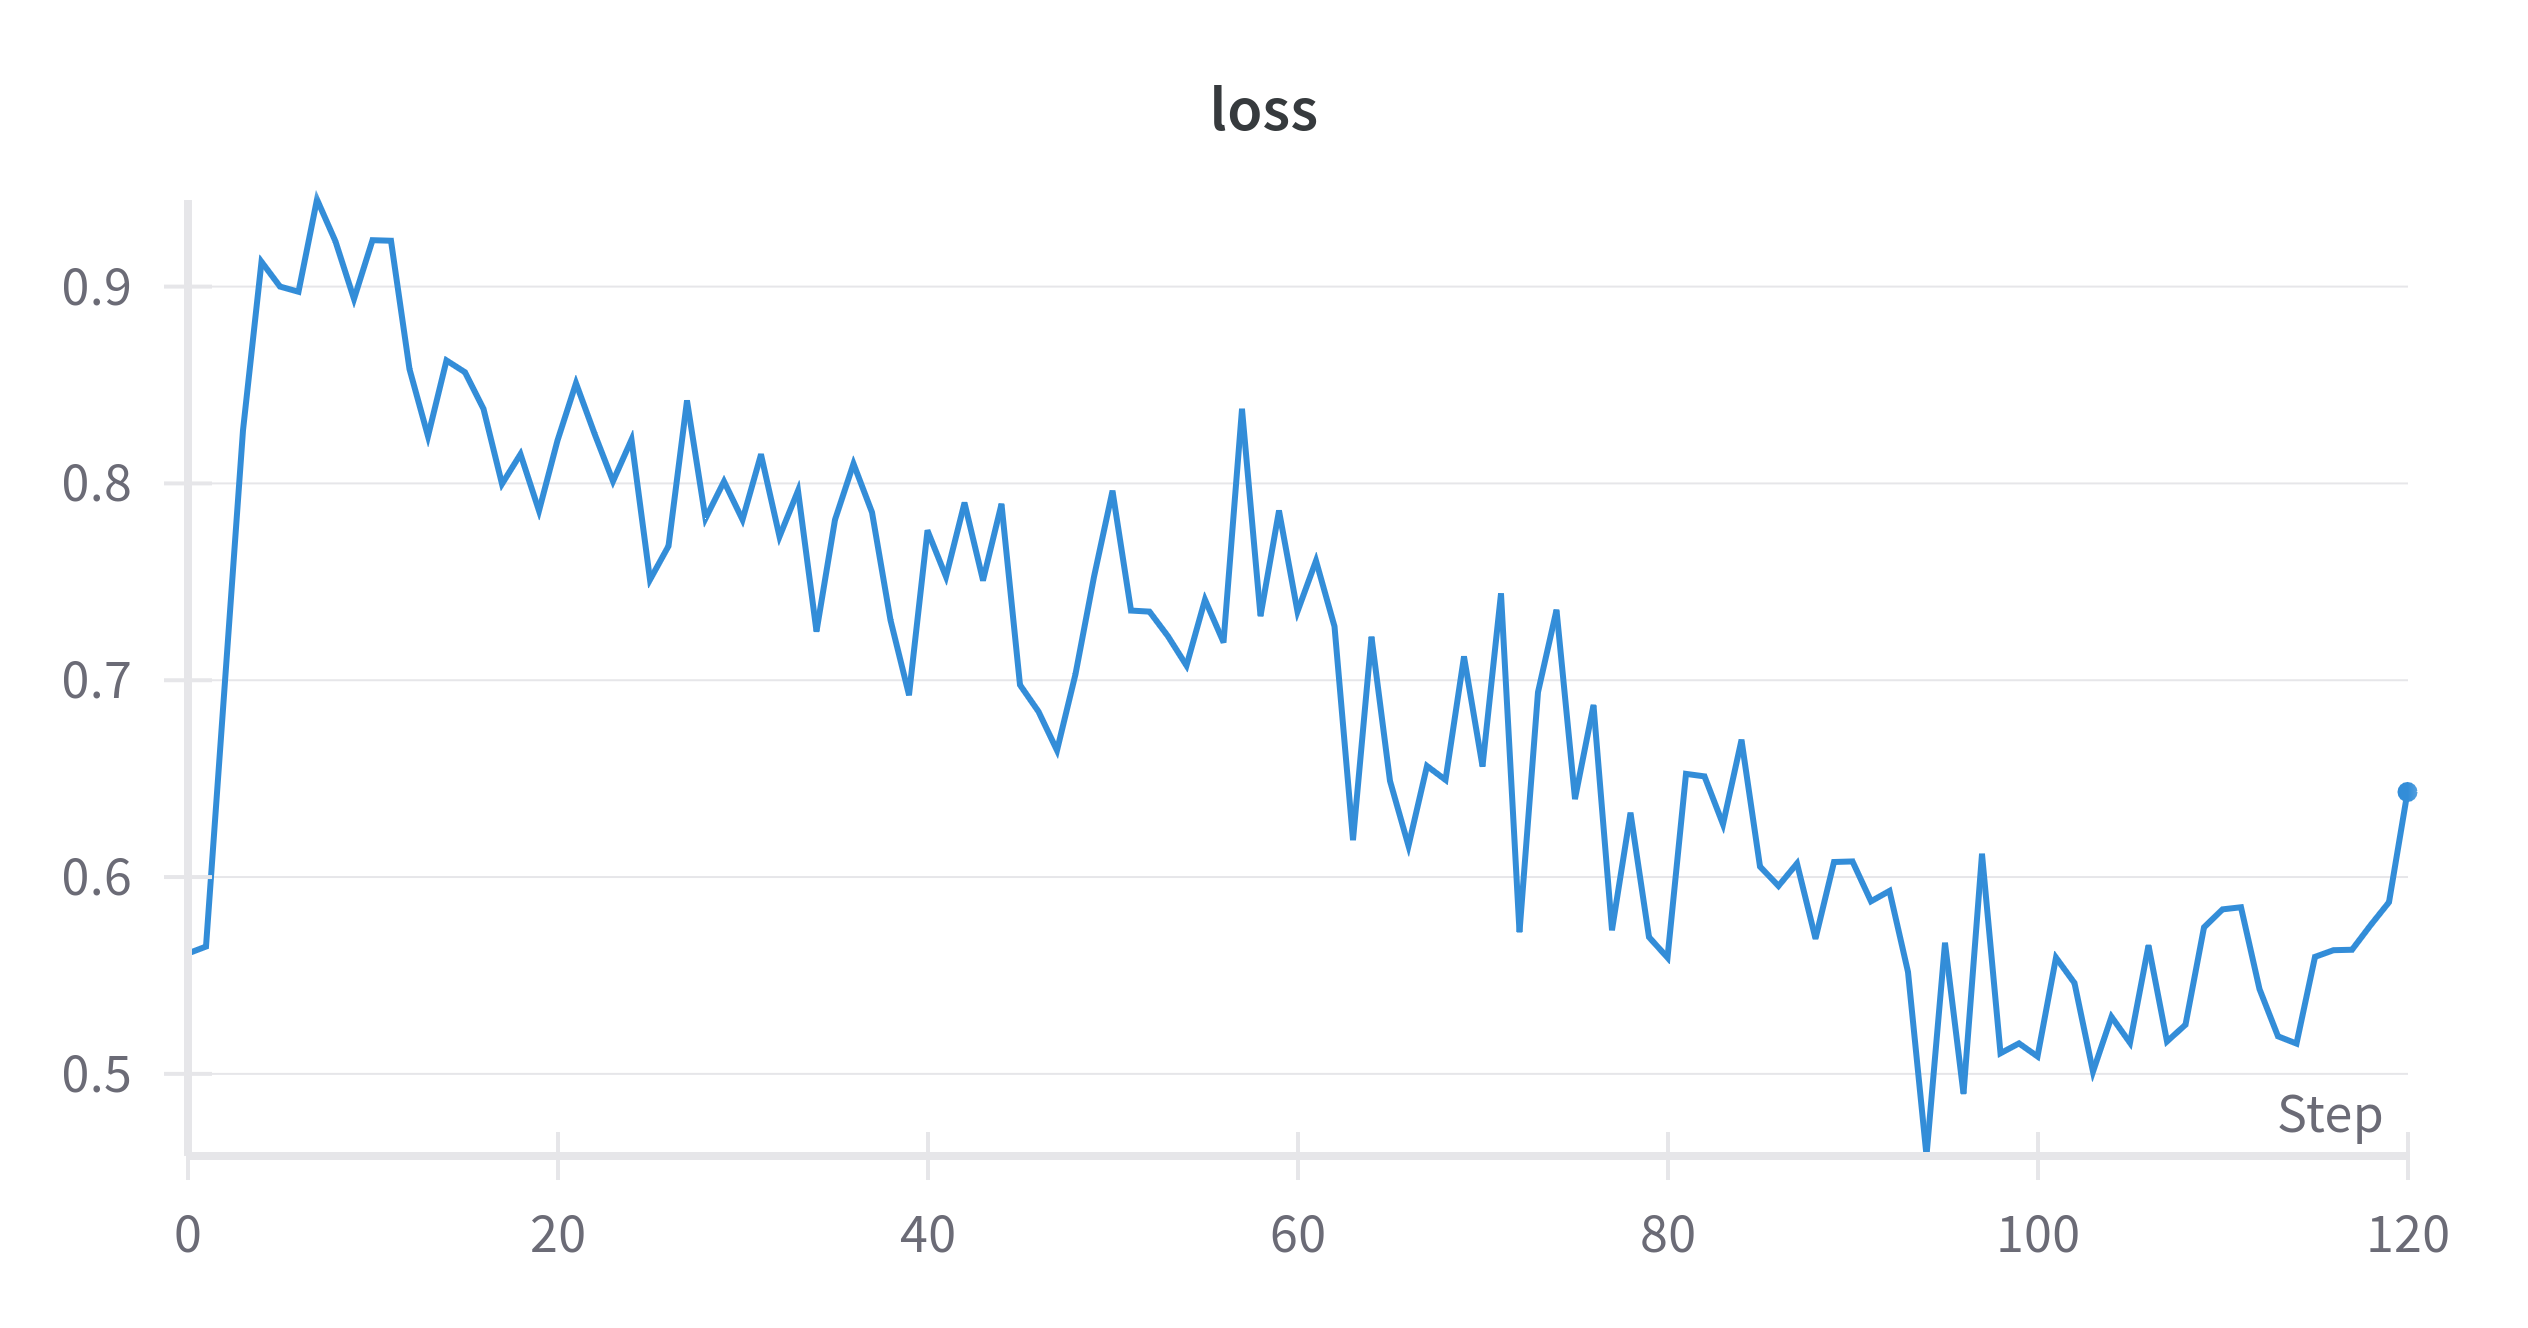
\includegraphics[width=\linewidth]{results/RAINBOW-loss.png}
    \caption{
        Loss curve for Rainbow Agent
    }
    \Description{Loss curve for Rainbow Agent}
    \label{fig:rainbowloss}
\end{figure*}


  \begin{figure*}[h]
    \centering
    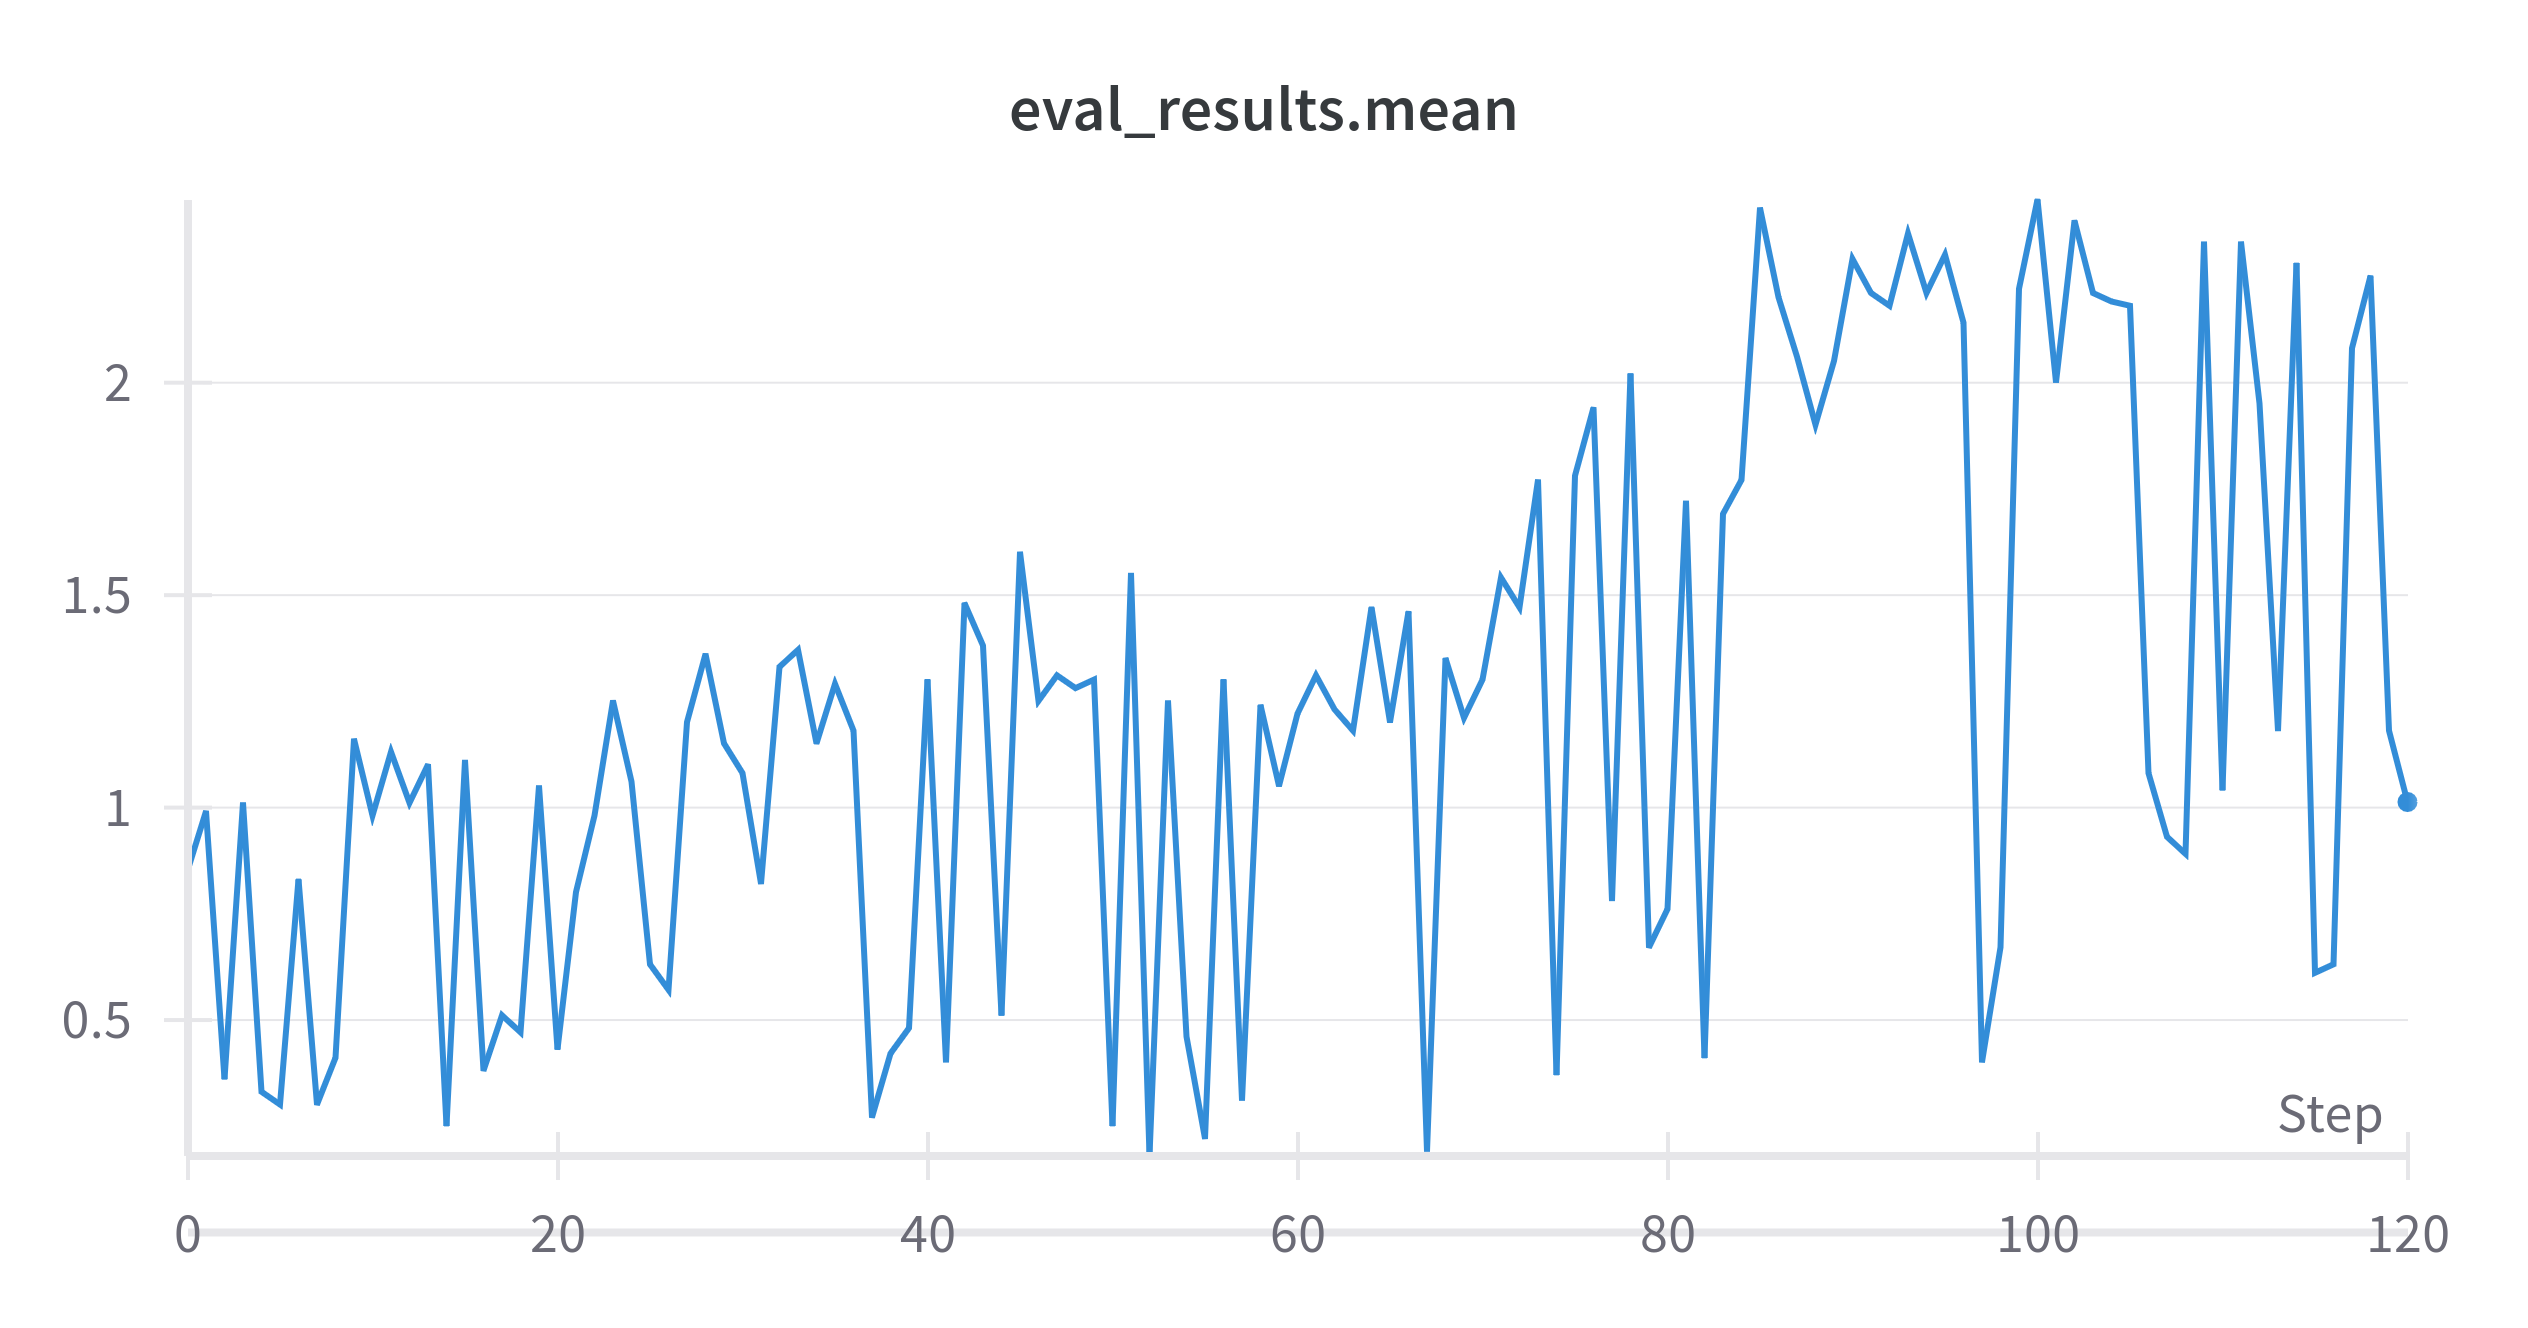
\includegraphics[width=\linewidth]{results/RAINBOW-3-mean.png}
    \caption{
      Training curve for Rainbow-3 Agent
    }
    \Description{Training curve for Rainbow-3 Agent}
    \label{fig:rainbow3}
  \end{figure*}
  \begin{figure*}[h]
    \centering
    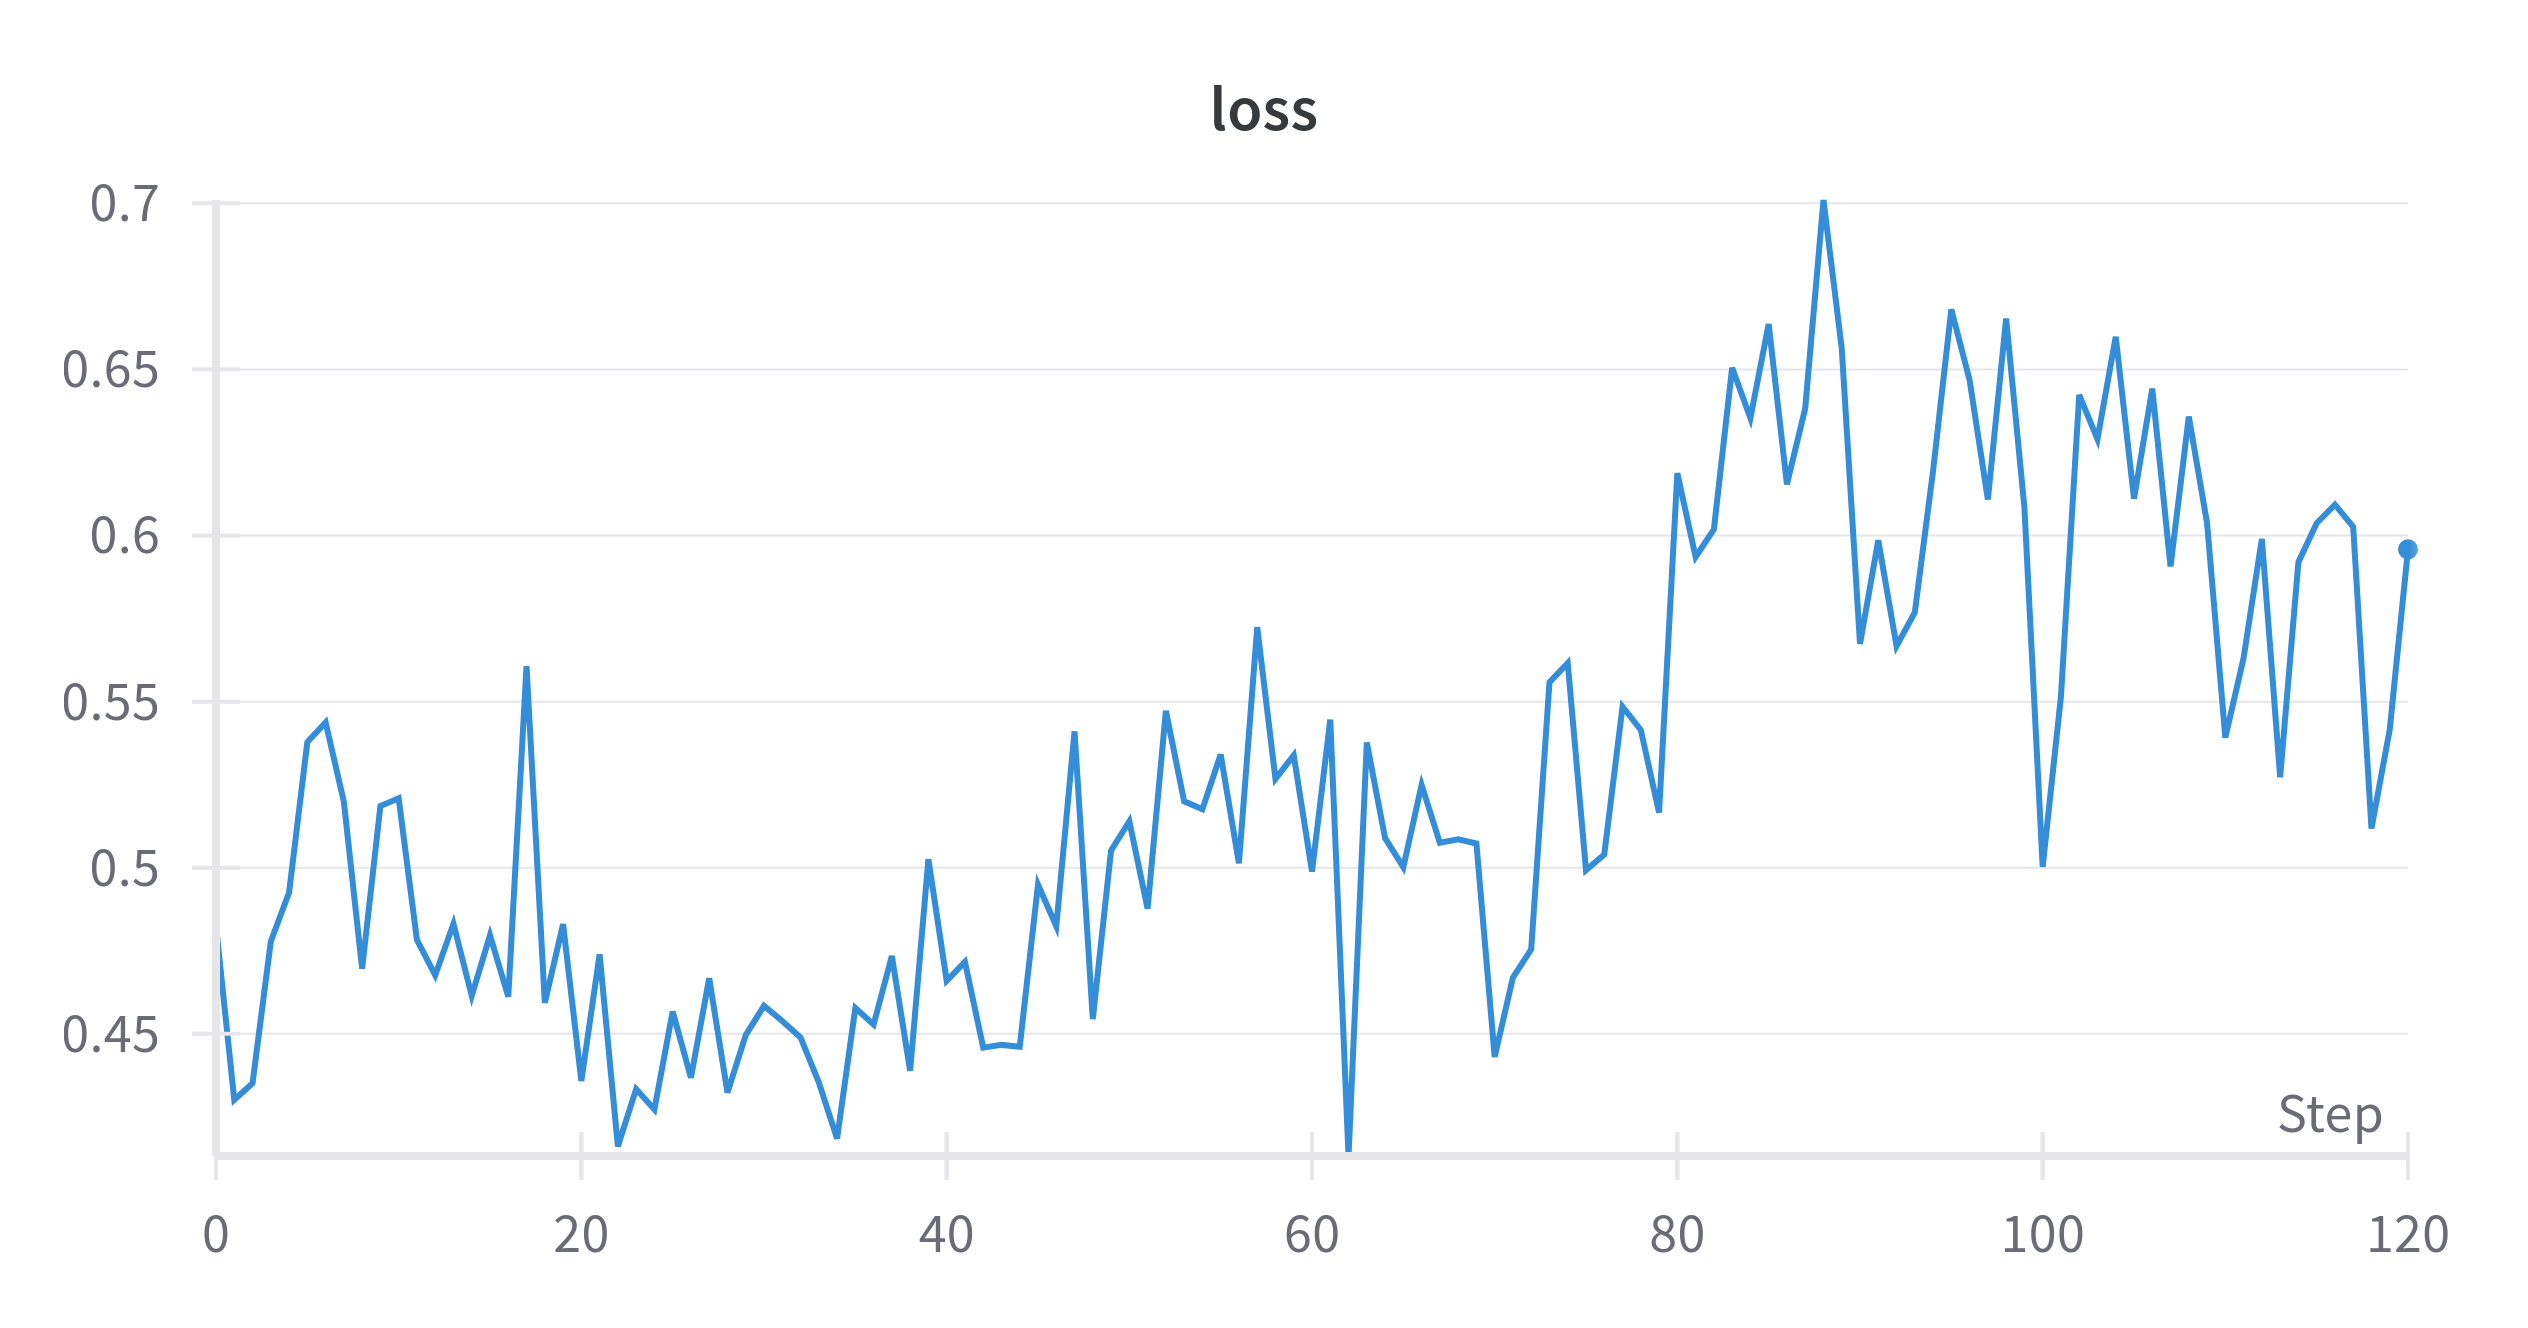
\includegraphics[width=\linewidth]{results/RAINBOW-3-loss.png}
    \caption{
        Loss curve for Rainbow-3 Agent
    }
    \Description{Loss curve for Rainbow-3 Agent}
    \label{fig:rainbow3loss}
\end{figure*}


\begin{figure*}[h]
  \centering
  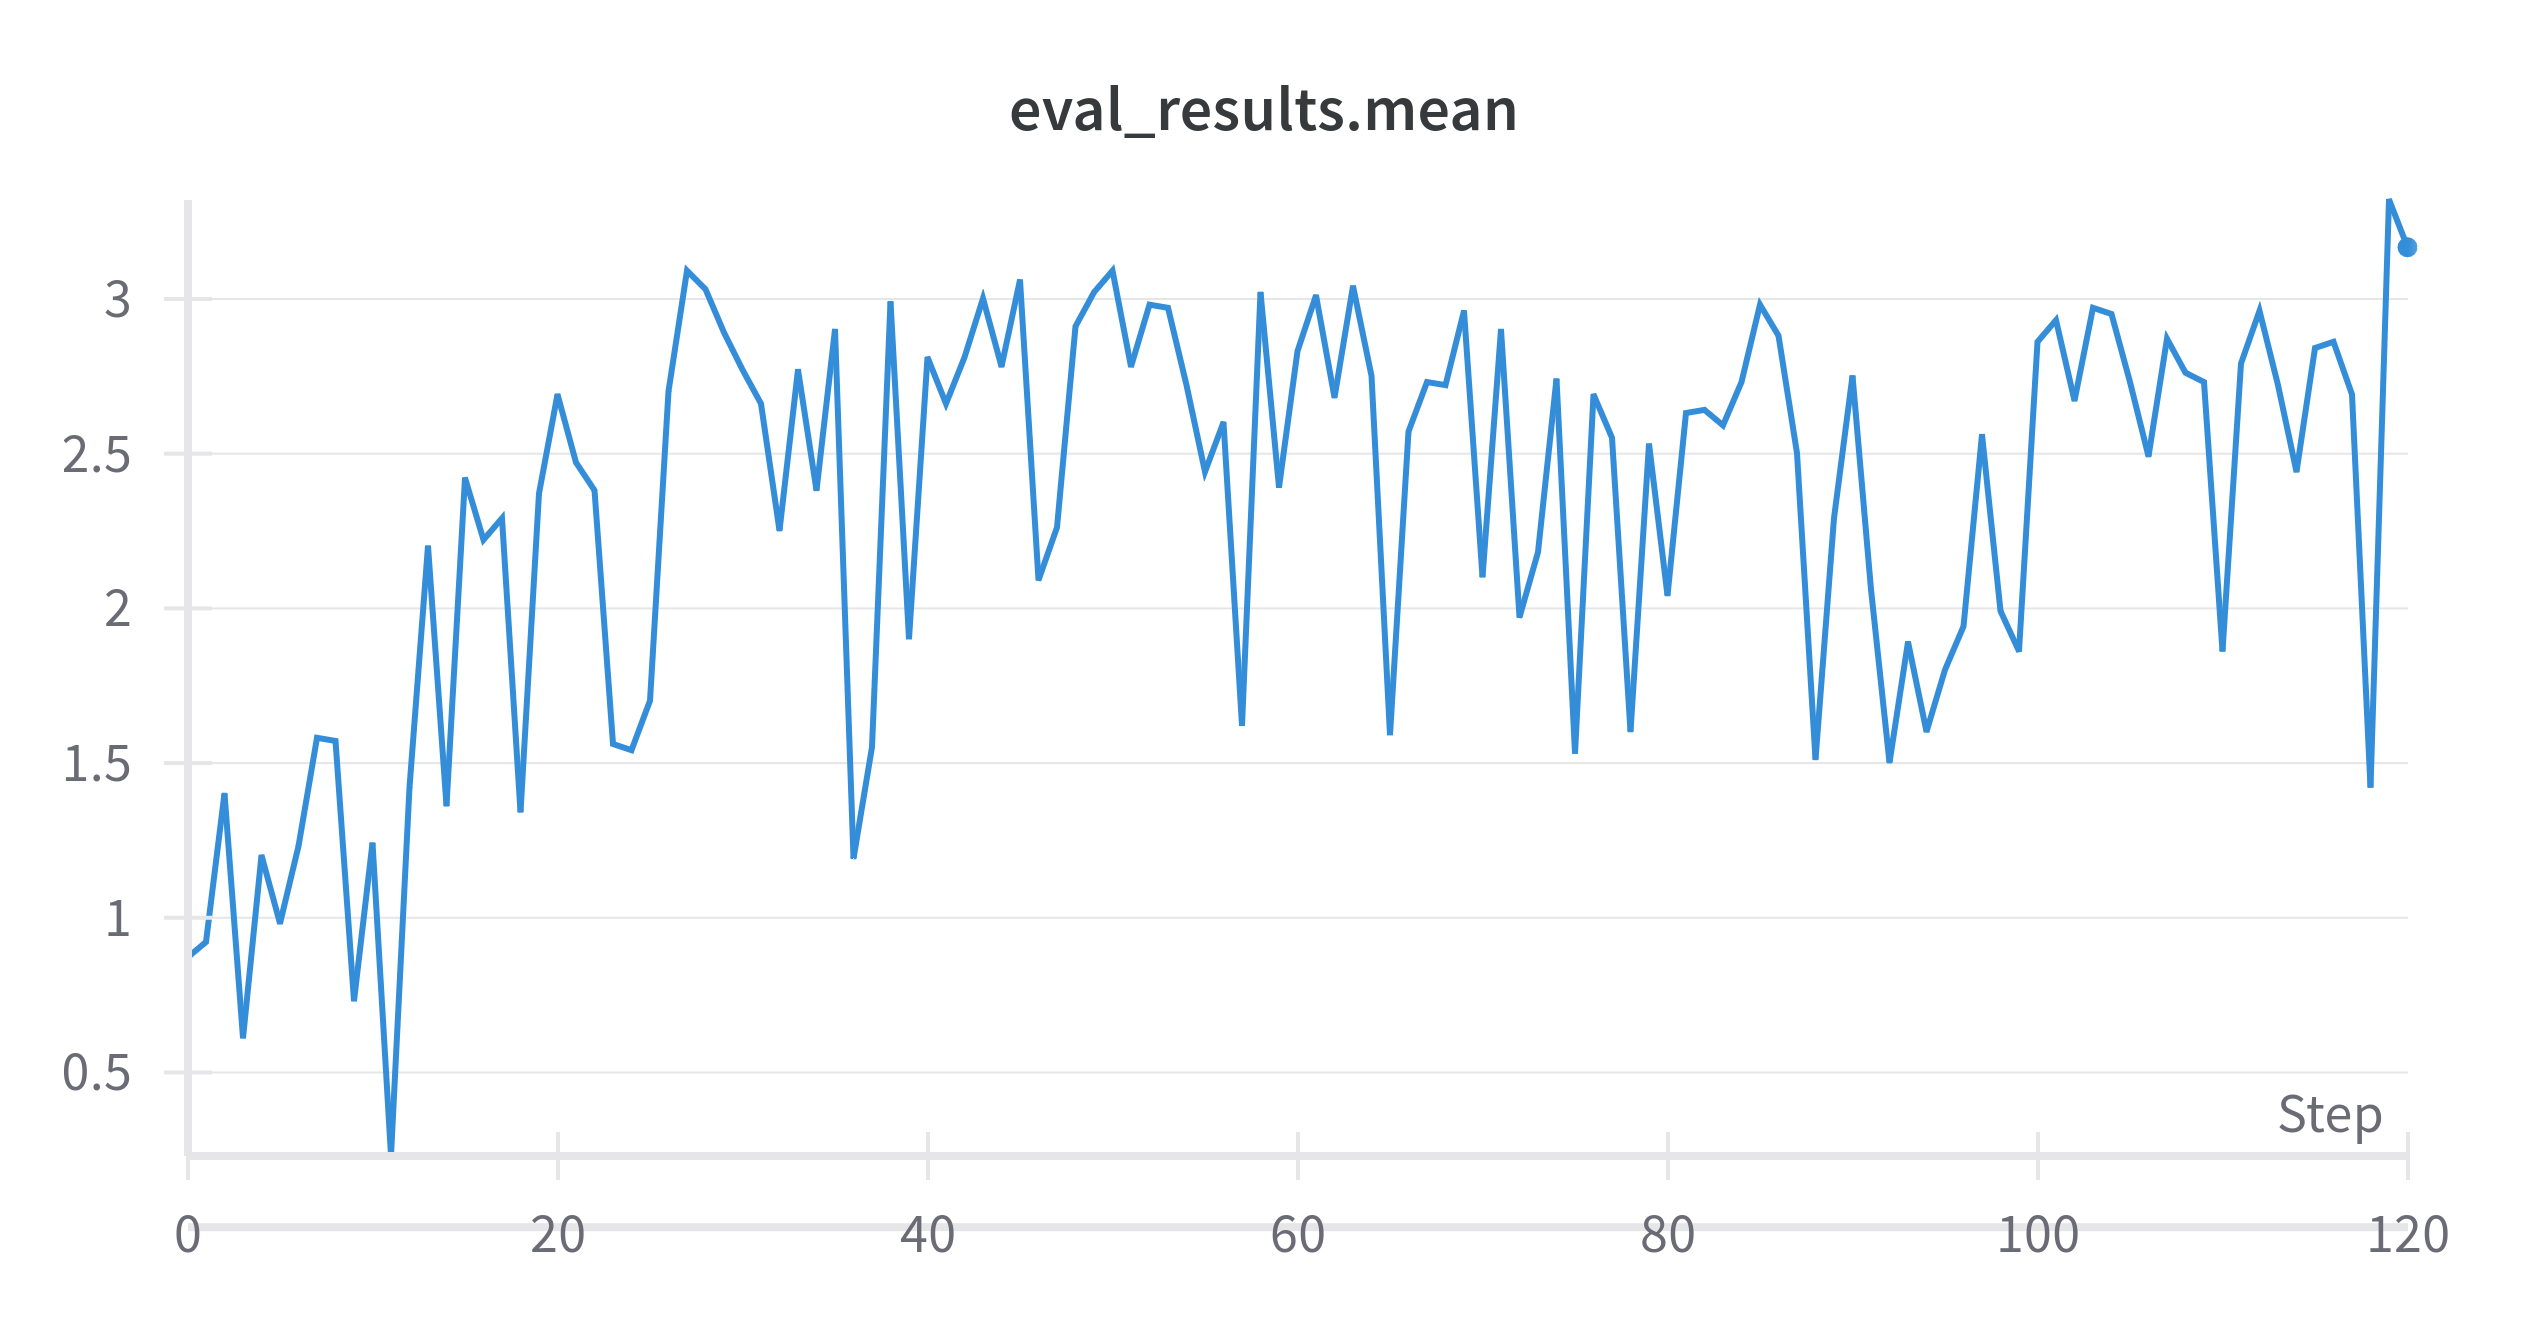
\includegraphics[width=\linewidth]{results/RAINBOW-5-mean.png}
  \caption{
    Training curve for Rainbow-5 Agent
  }
  \Description{Training curve for Rainbow-5 Agent}
  \label{fig:rainbow5}
\end{figure*}

\begin{figure*}[h]
  \centering
  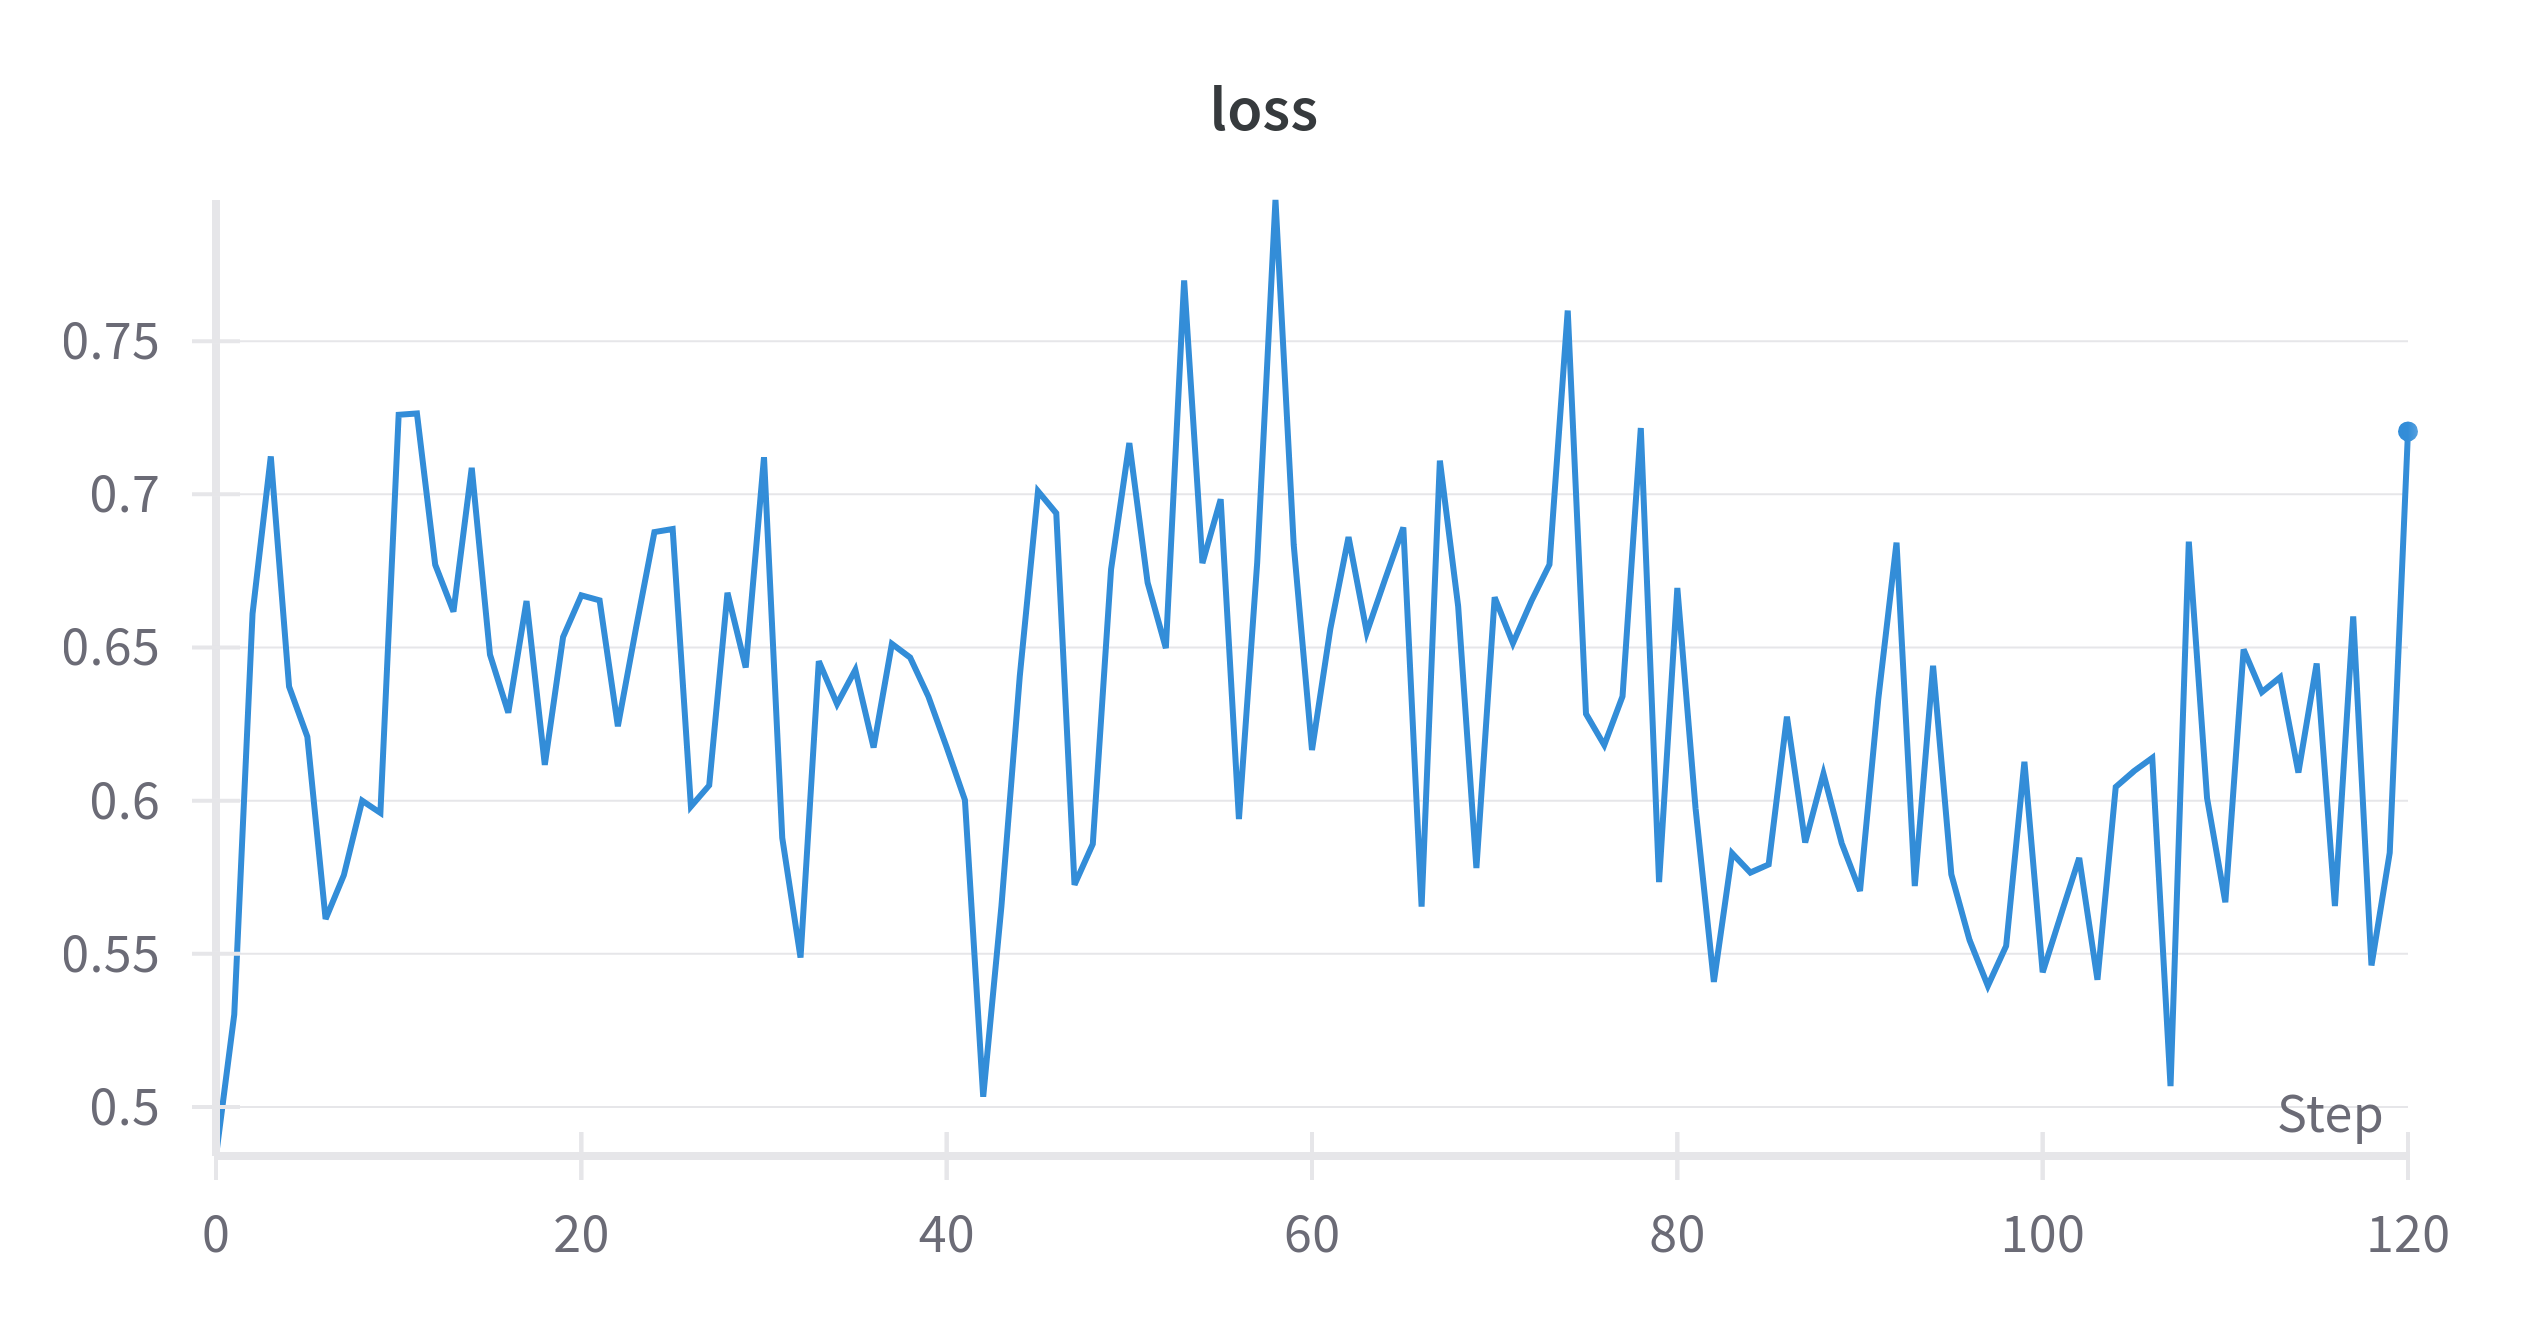
\includegraphics[width=\linewidth]{results/RAINBOW-5-loss.png}
  \caption{
      Loss curve for Rainbow-5 Agent
  }
  \Description{Loss curve for Rainbow-5 Agent}
  \label{fig:rainbow5loss}
\end{figure*}


  \begin{figure*}[h]
    \centering
    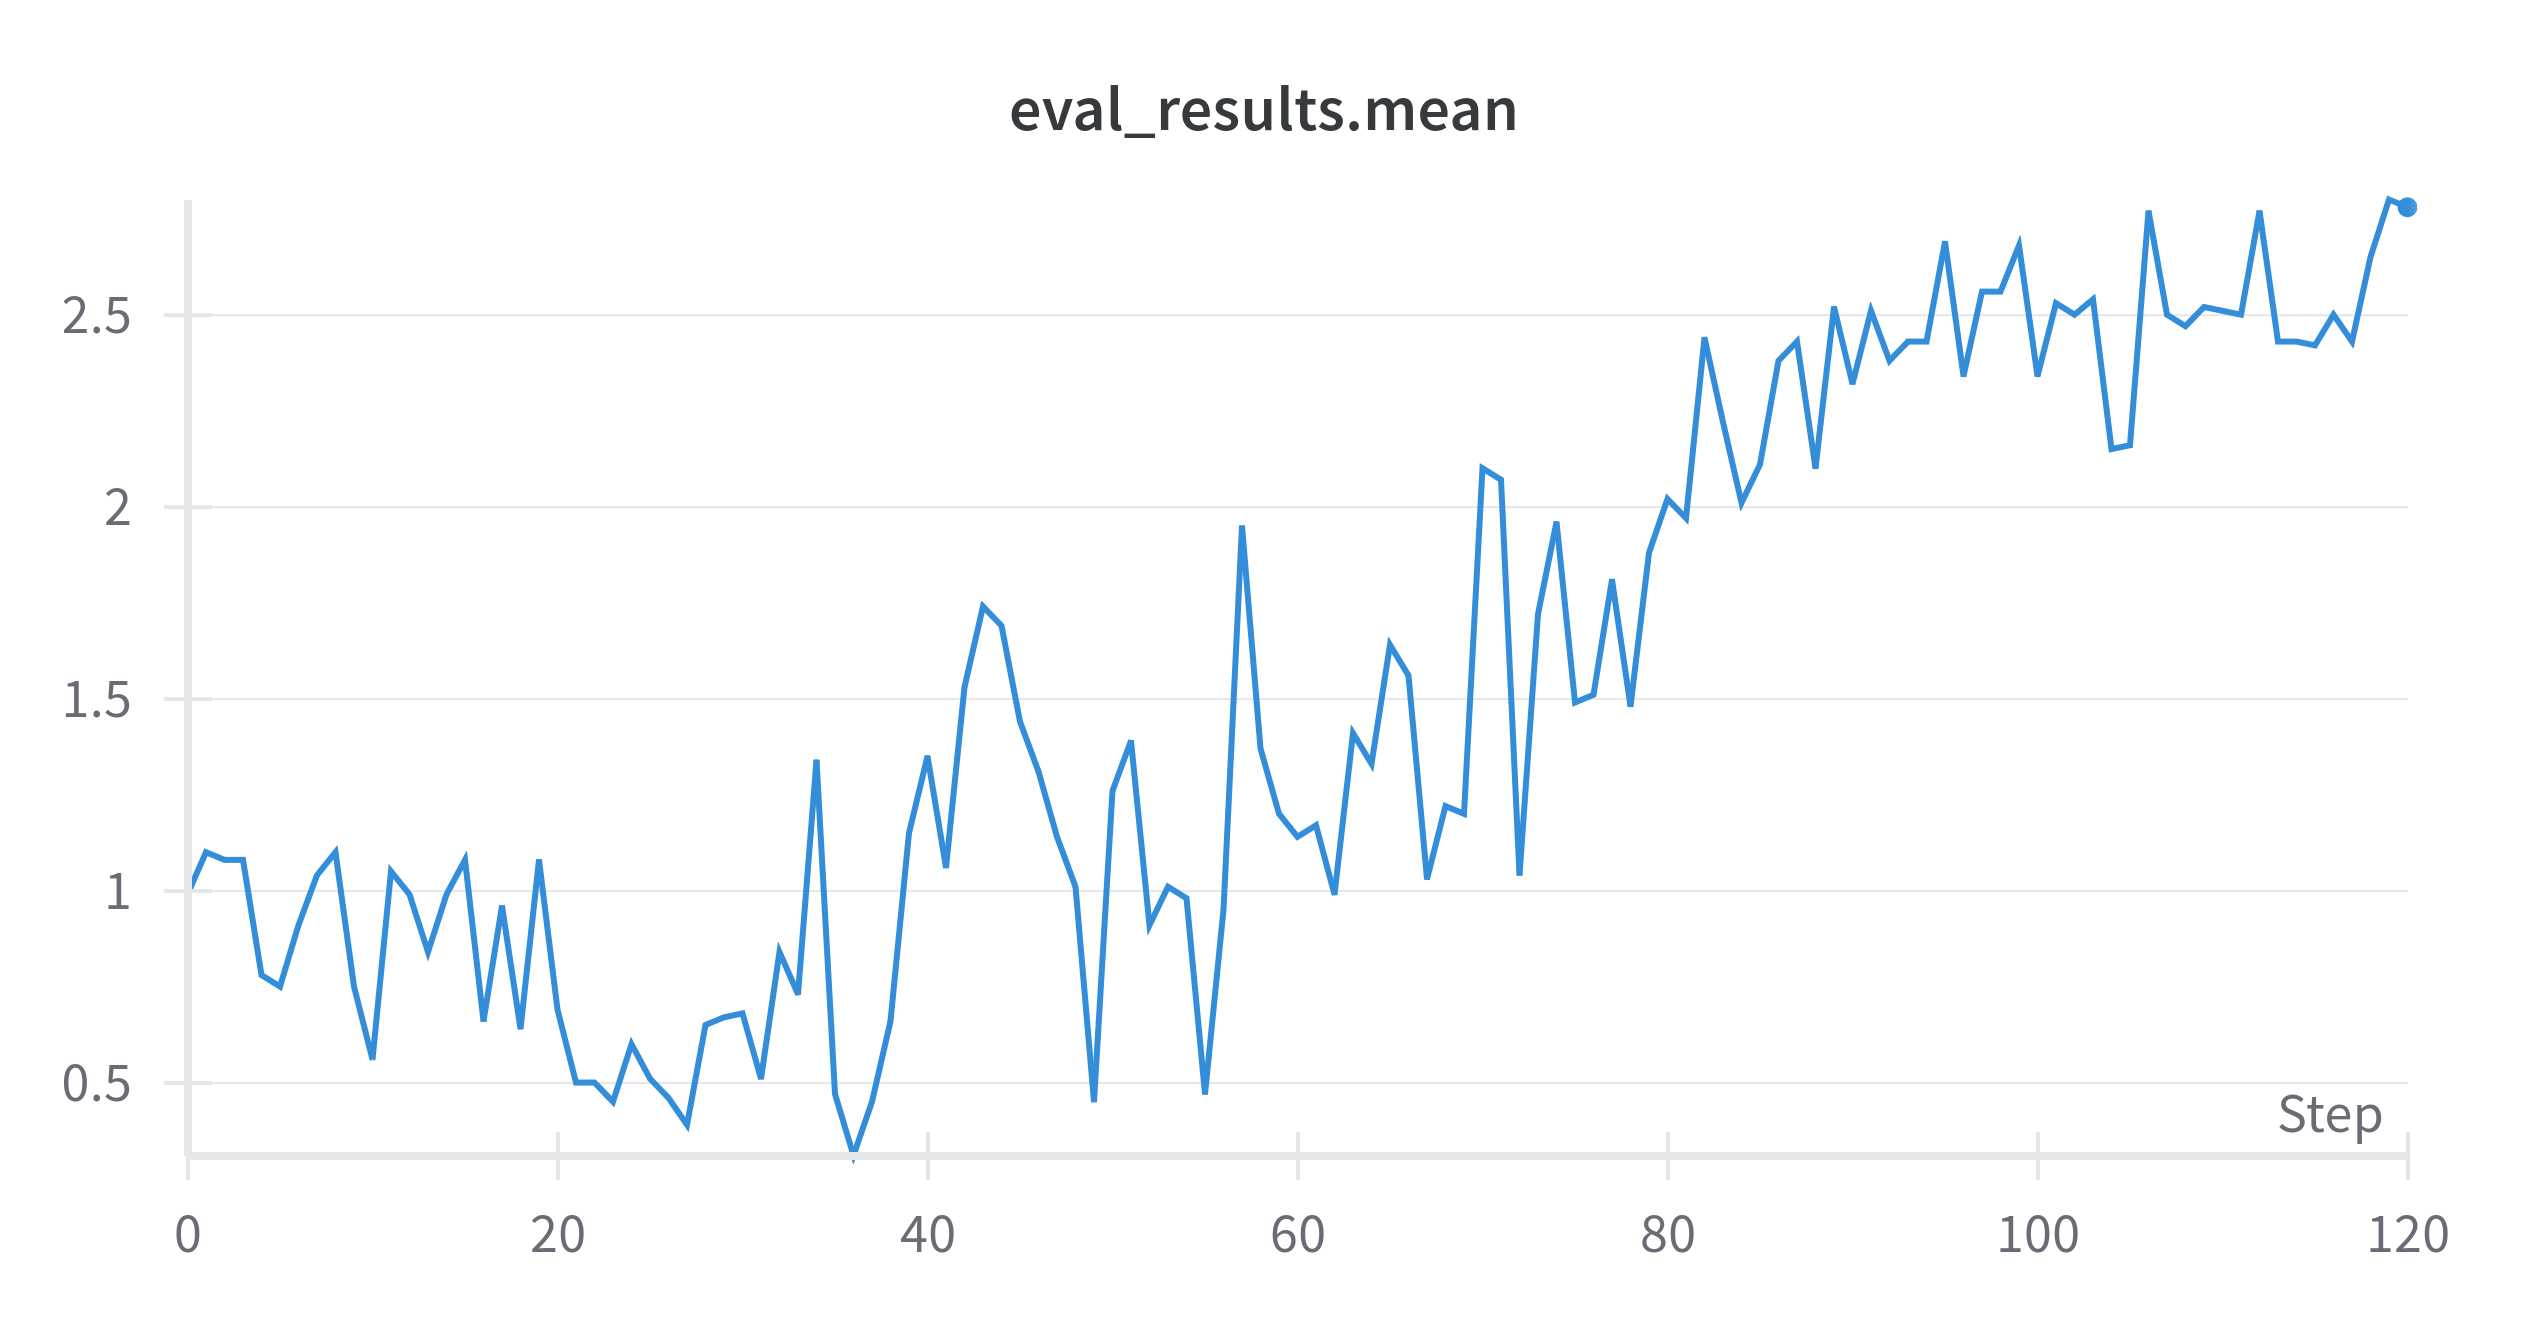
\includegraphics[width=\linewidth]{results/Distributed-mean.png}
    \caption{
      Training curve for Distributed Agent
    }
    \Description{Training curve for Distributed Agent}
    \label{fig:distributed}
  \end{figure*}


\begin{figure*}[h]
  \centering
  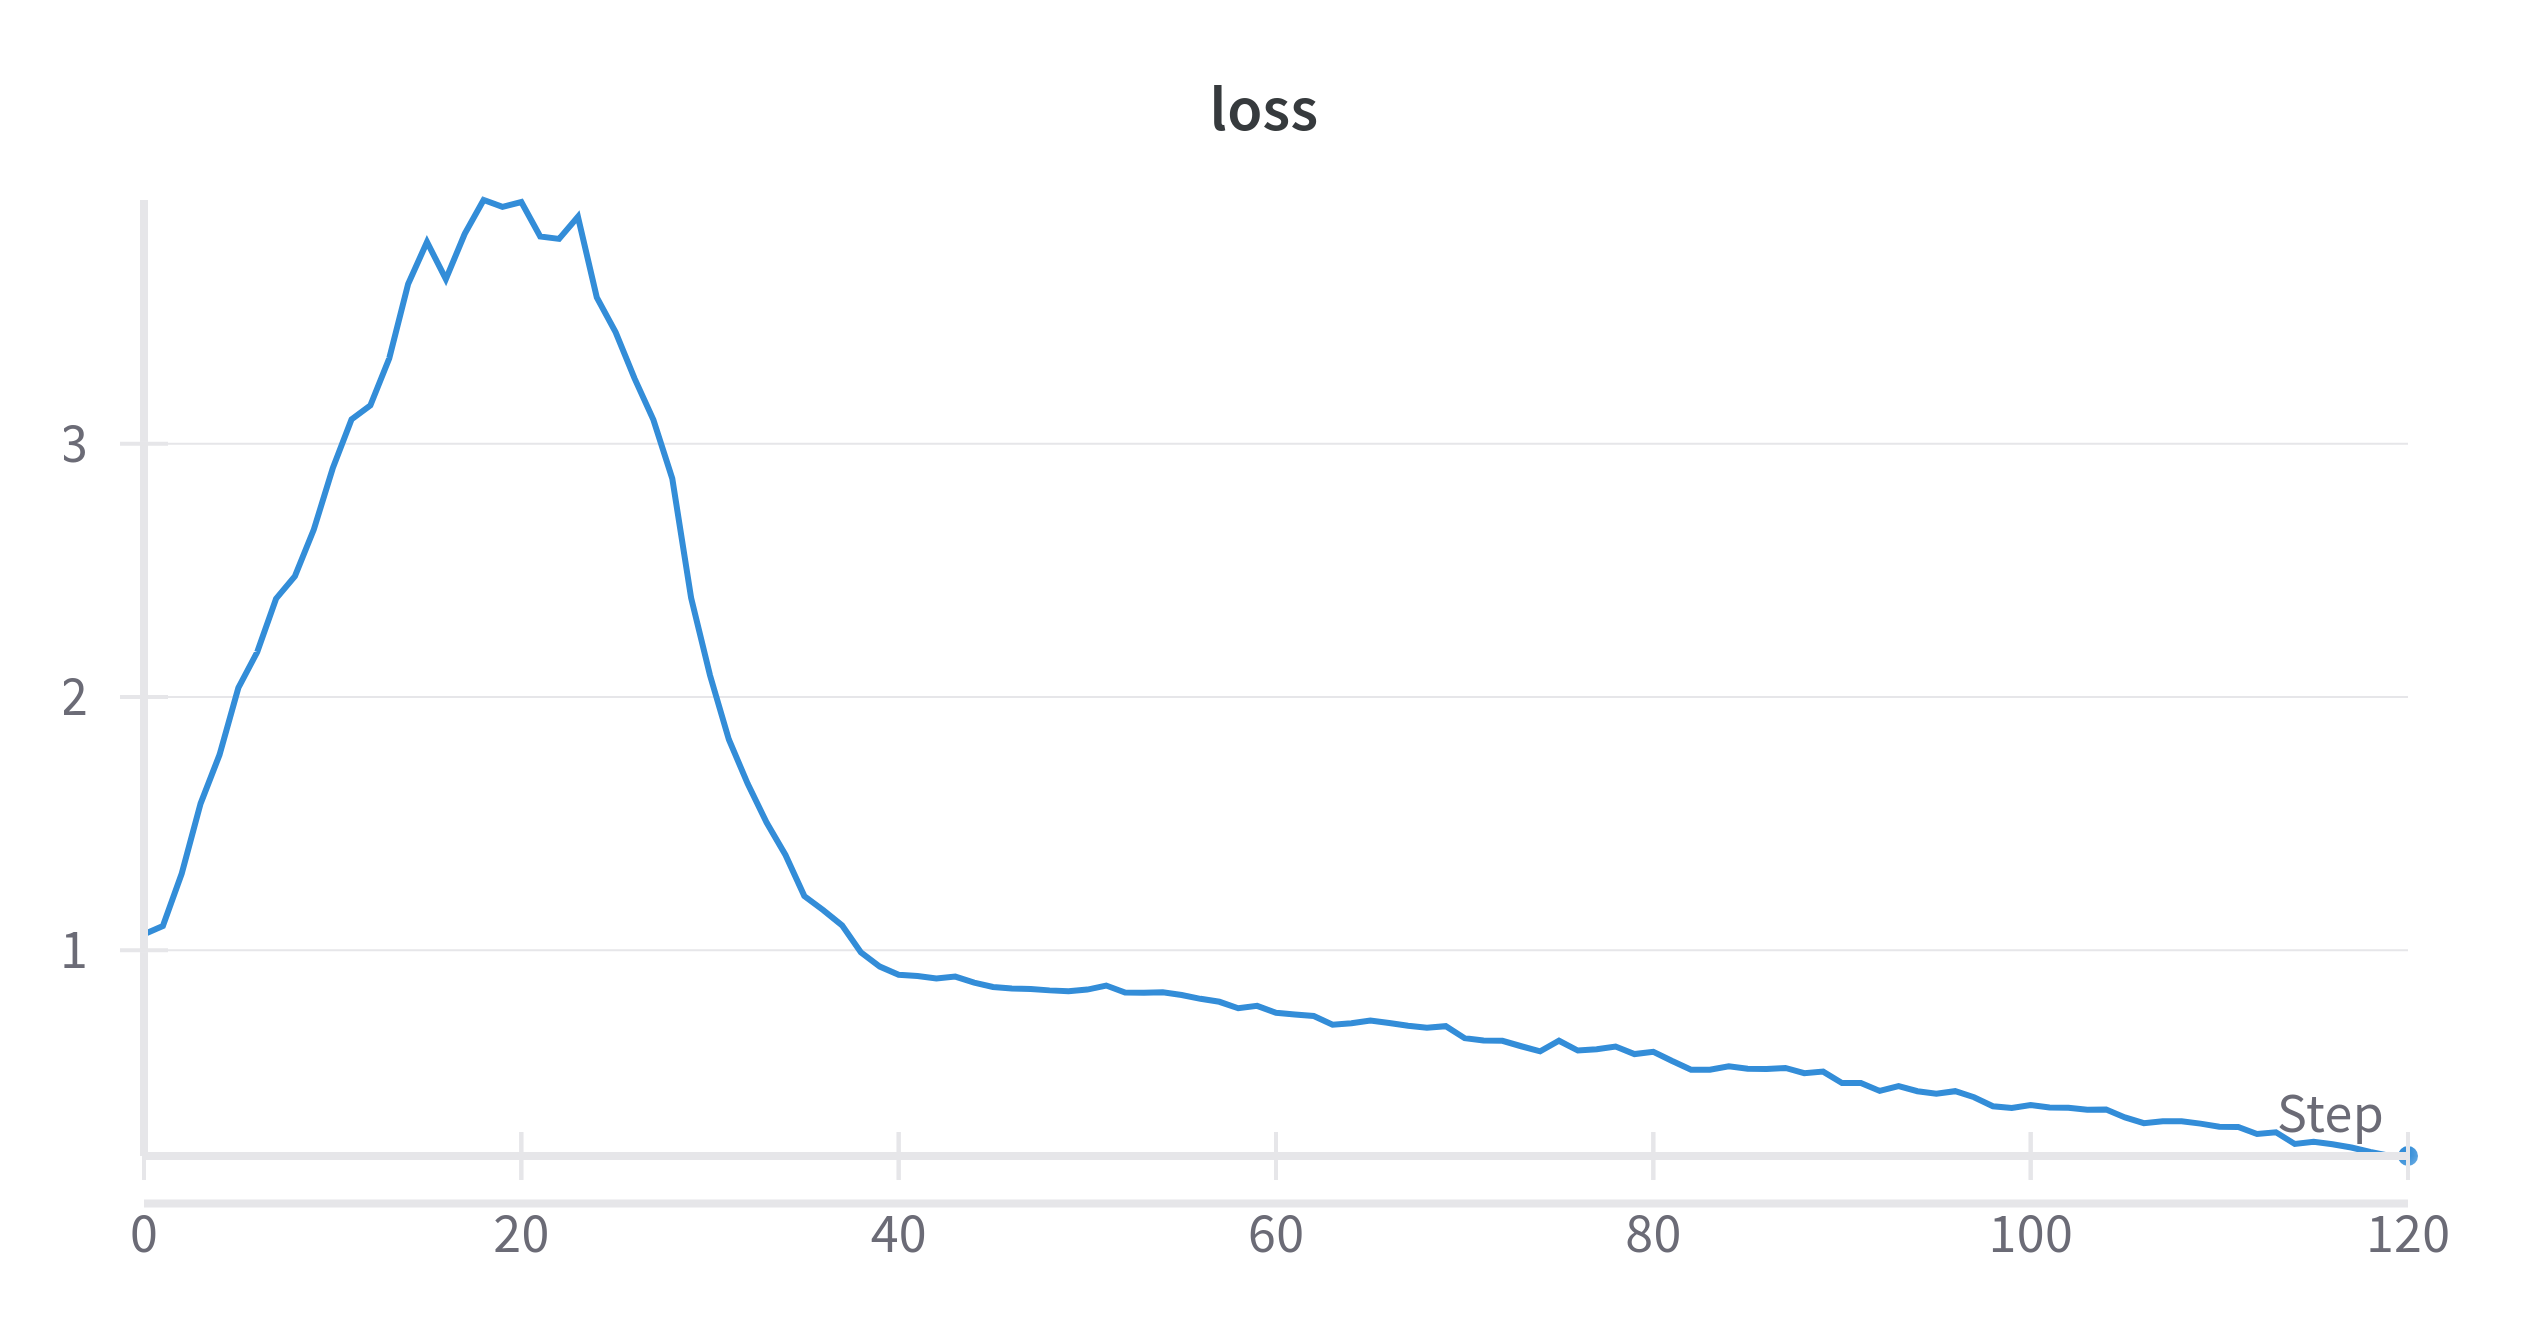
\includegraphics[width=\linewidth]{results/Distributed-loss.png}
  \caption{
      Loss curve for Distributed Agent
  }
  \Description{Loss curve for Distributed Agent}
  \label{fig:distributedloss}
\end{figure*}

  
  \begin{figure*}[h]
    \centering
    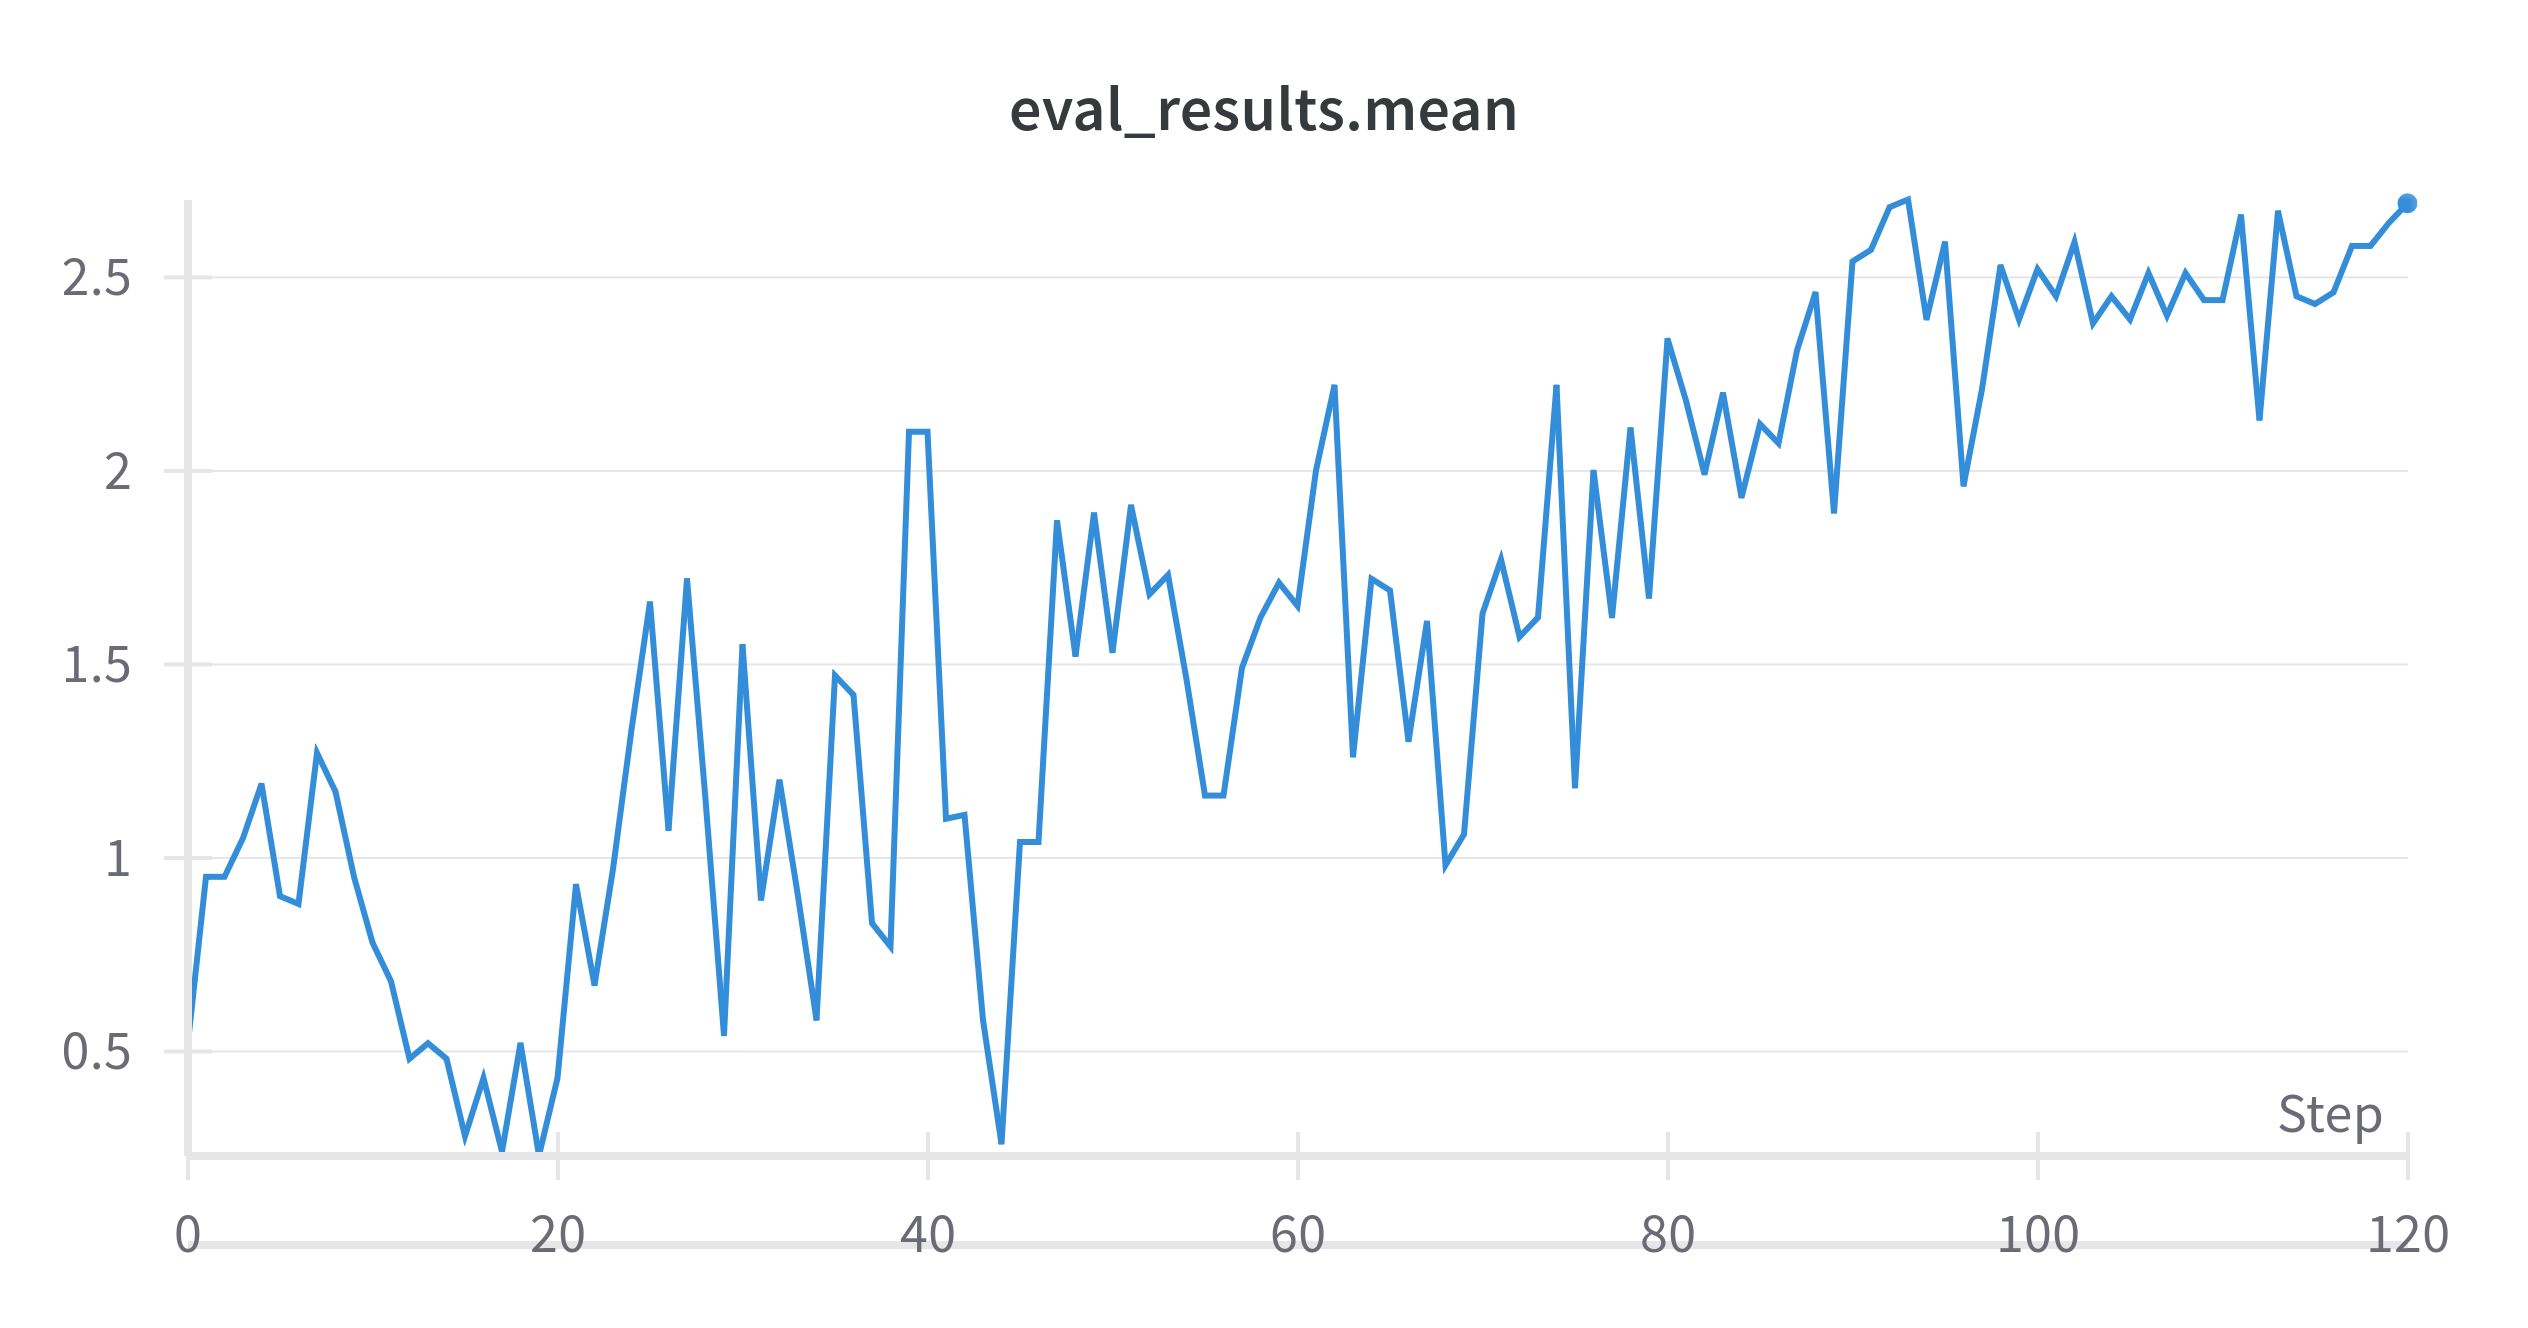
\includegraphics[width=\linewidth]{results/SAD-mean.png}
    \caption{
      Training curve for SAD Agent
    }
    \Description{Training curve for SAD Agent}
    \label{fig:sad}
  \end{figure*}
  
\begin{figure*}[h]
  \centering
  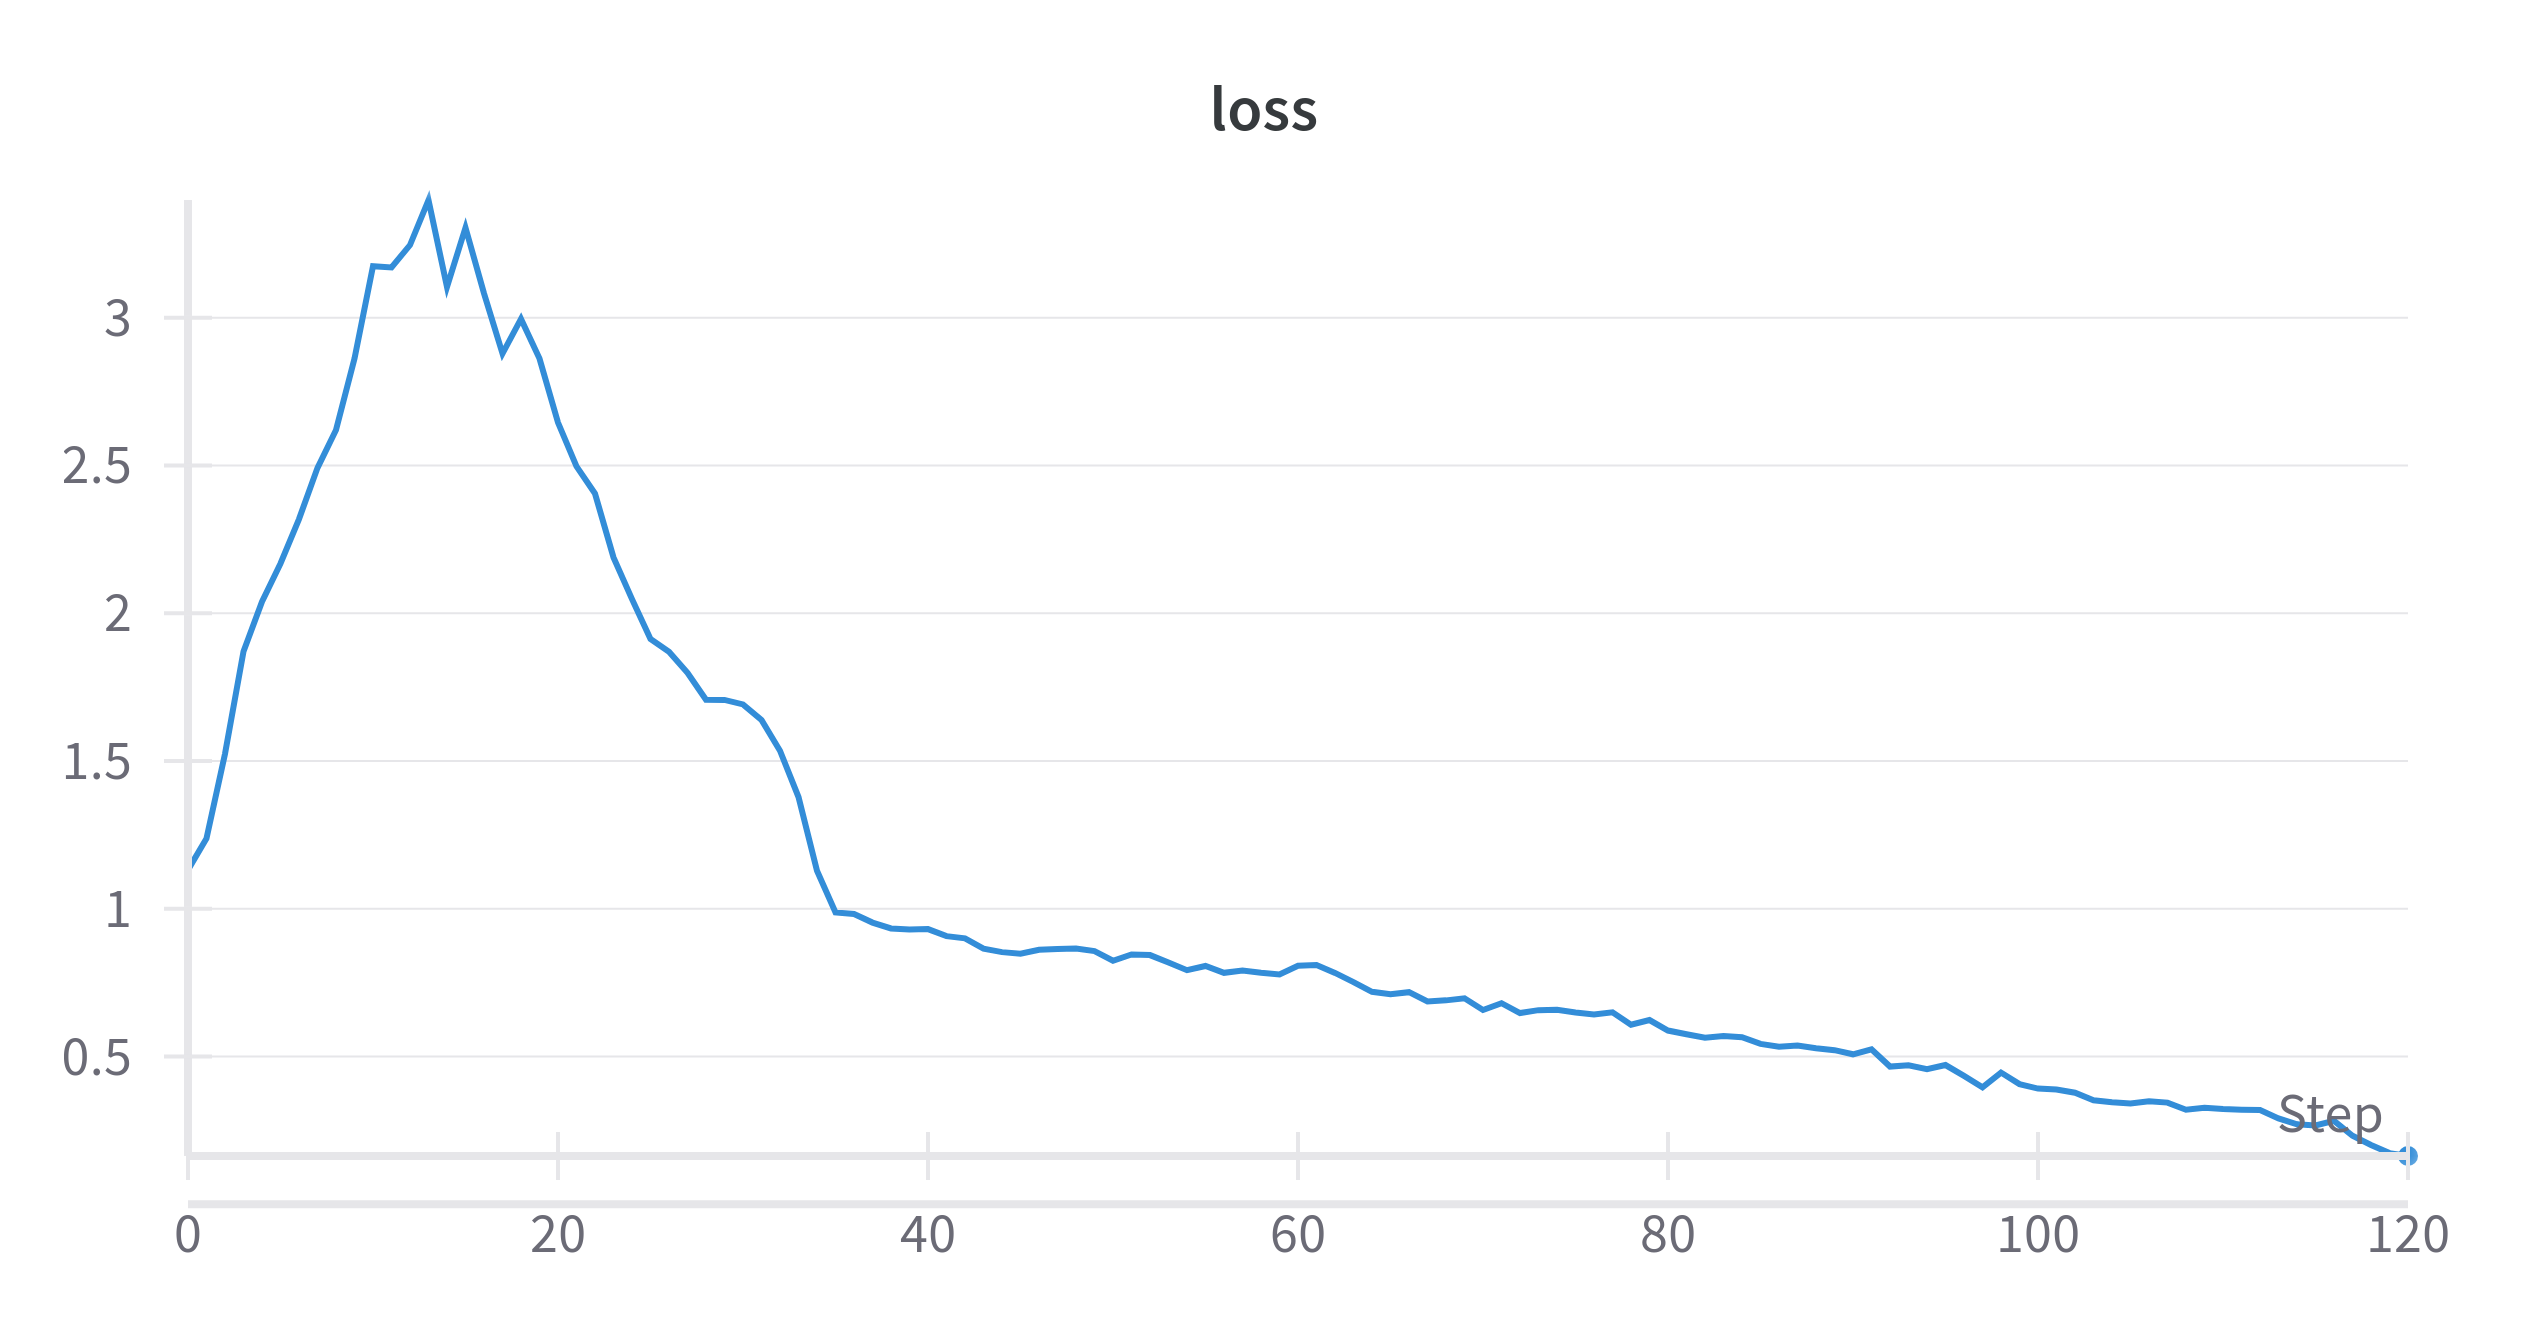
\includegraphics[width=\linewidth]{results/SAD-loss.png}
  \caption{
      Loss curve for SAD Agent
  }
  \Description{Loss curve for SAD Agent}
  \label{fig:sadloss}
\end{figure*}


  \begin{figure*}[h]
    \centering
    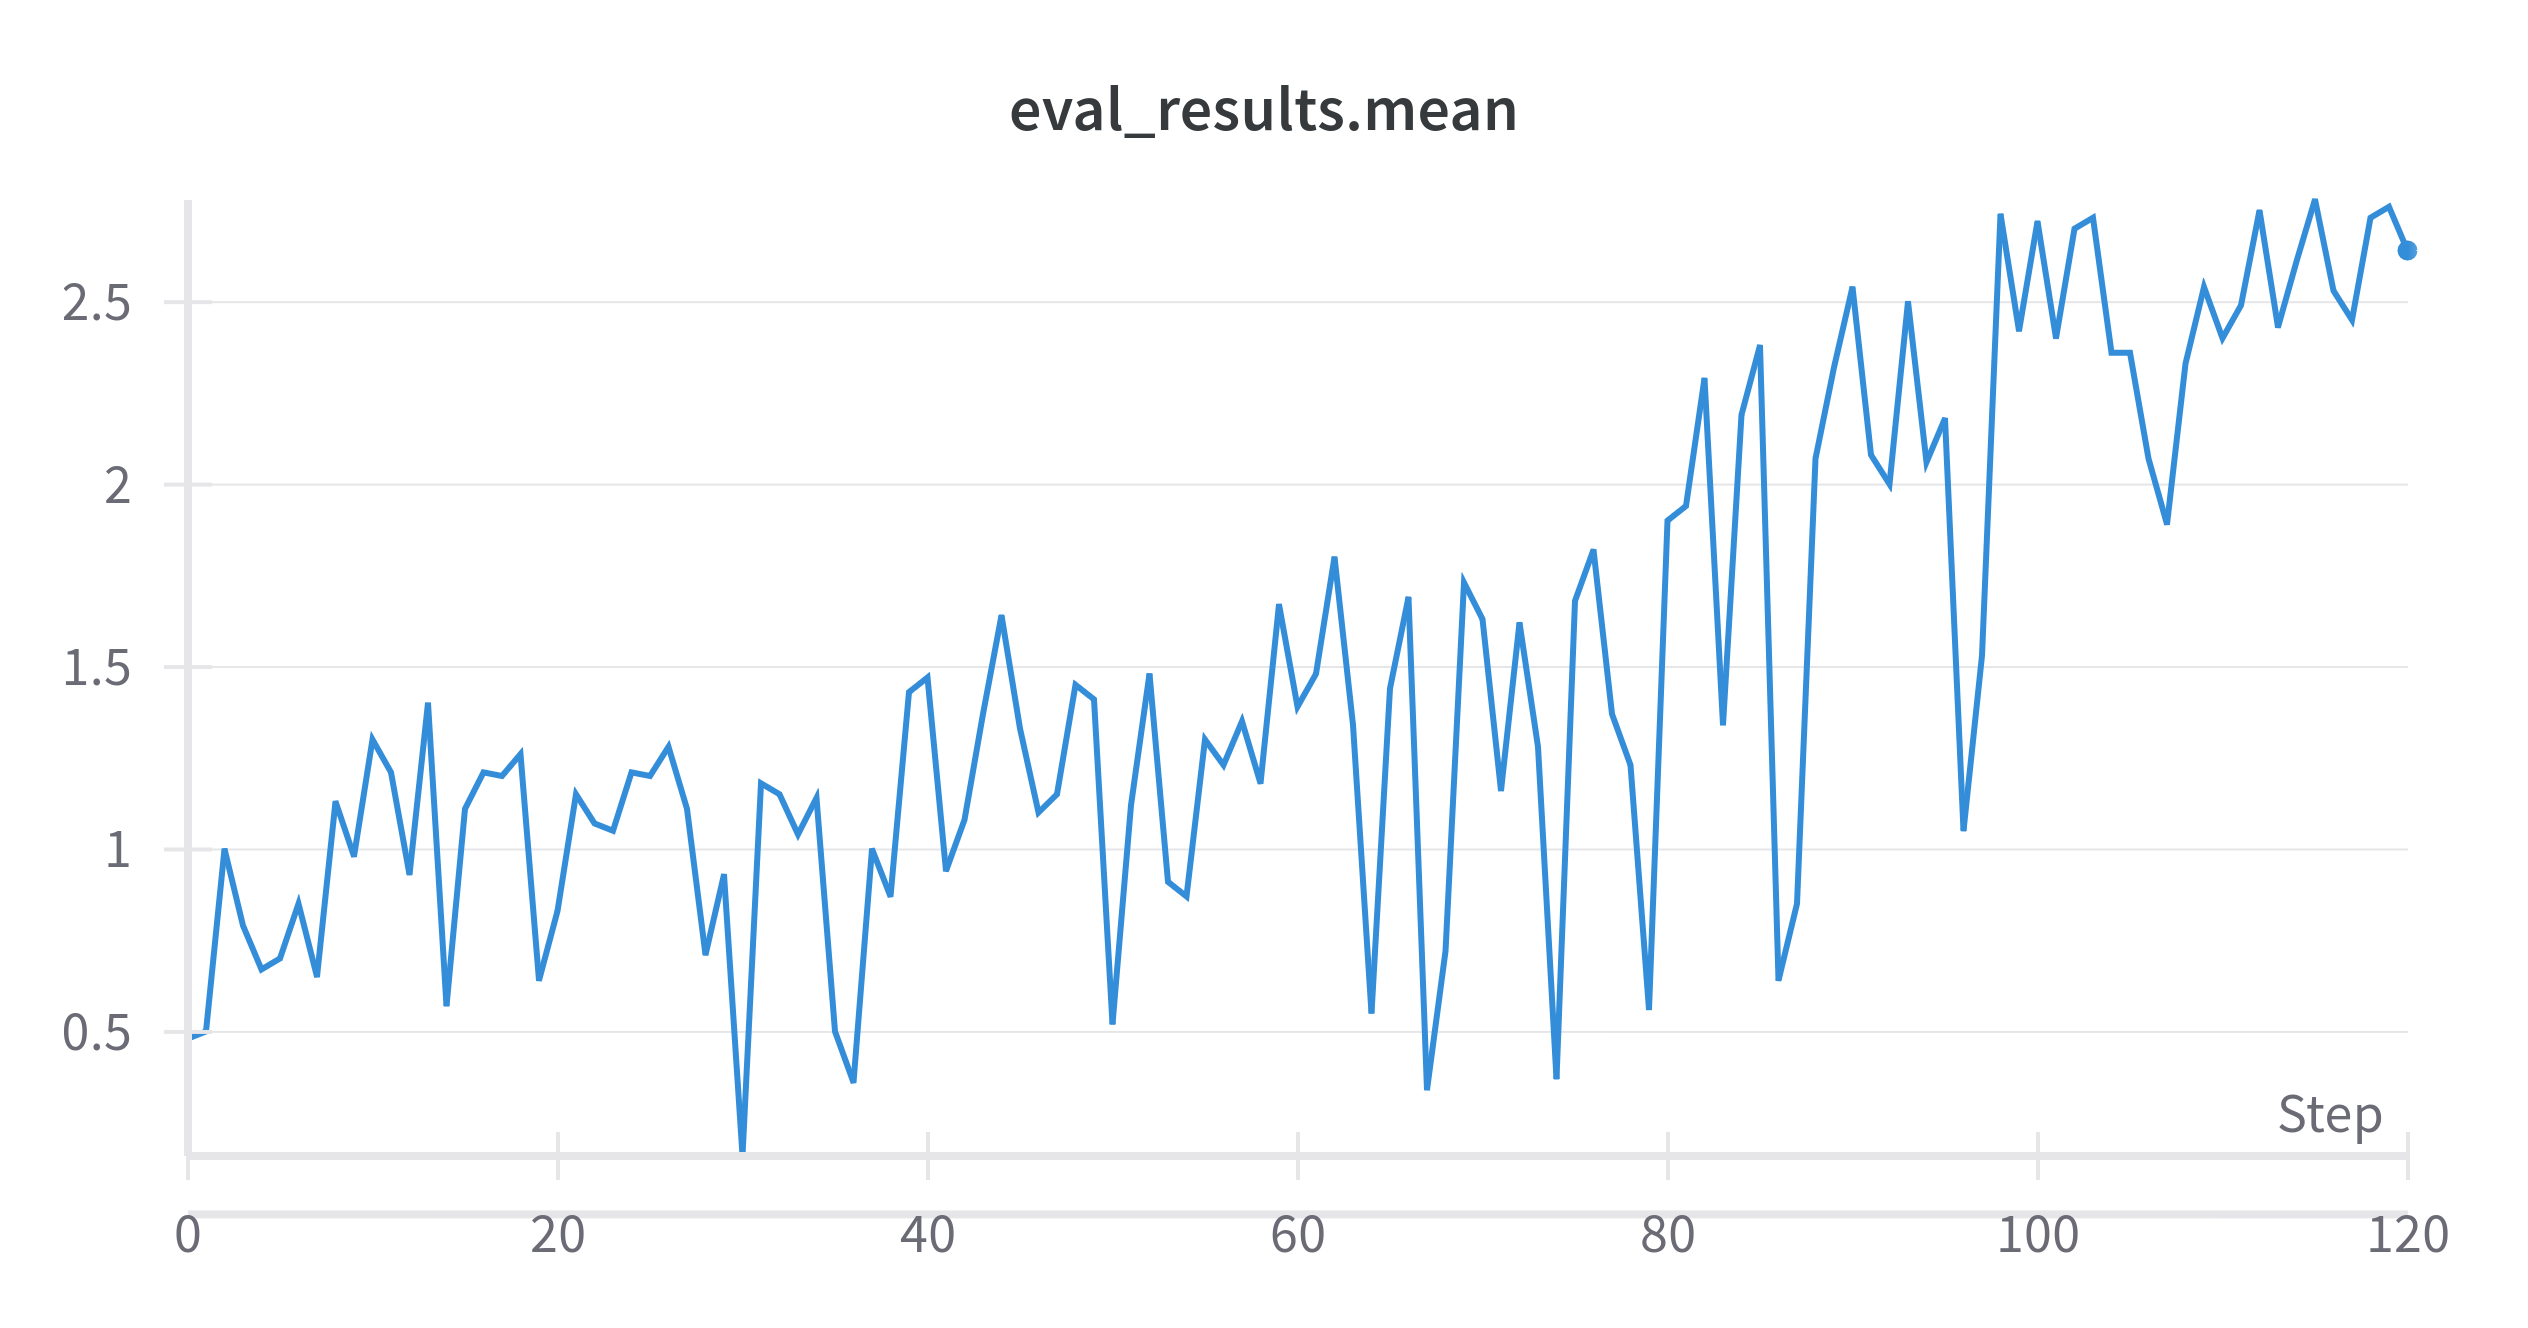
\includegraphics[width=\linewidth]{results/SAD-3-mean.png}
    \caption{
      Training curve for SAD-3 Agent
    }
    \Description{Training curve for SAD-3 Agent}
    \label{fig:sad3mean}
  \end{figure*}

  \begin{figure*}[h]
    \centering
    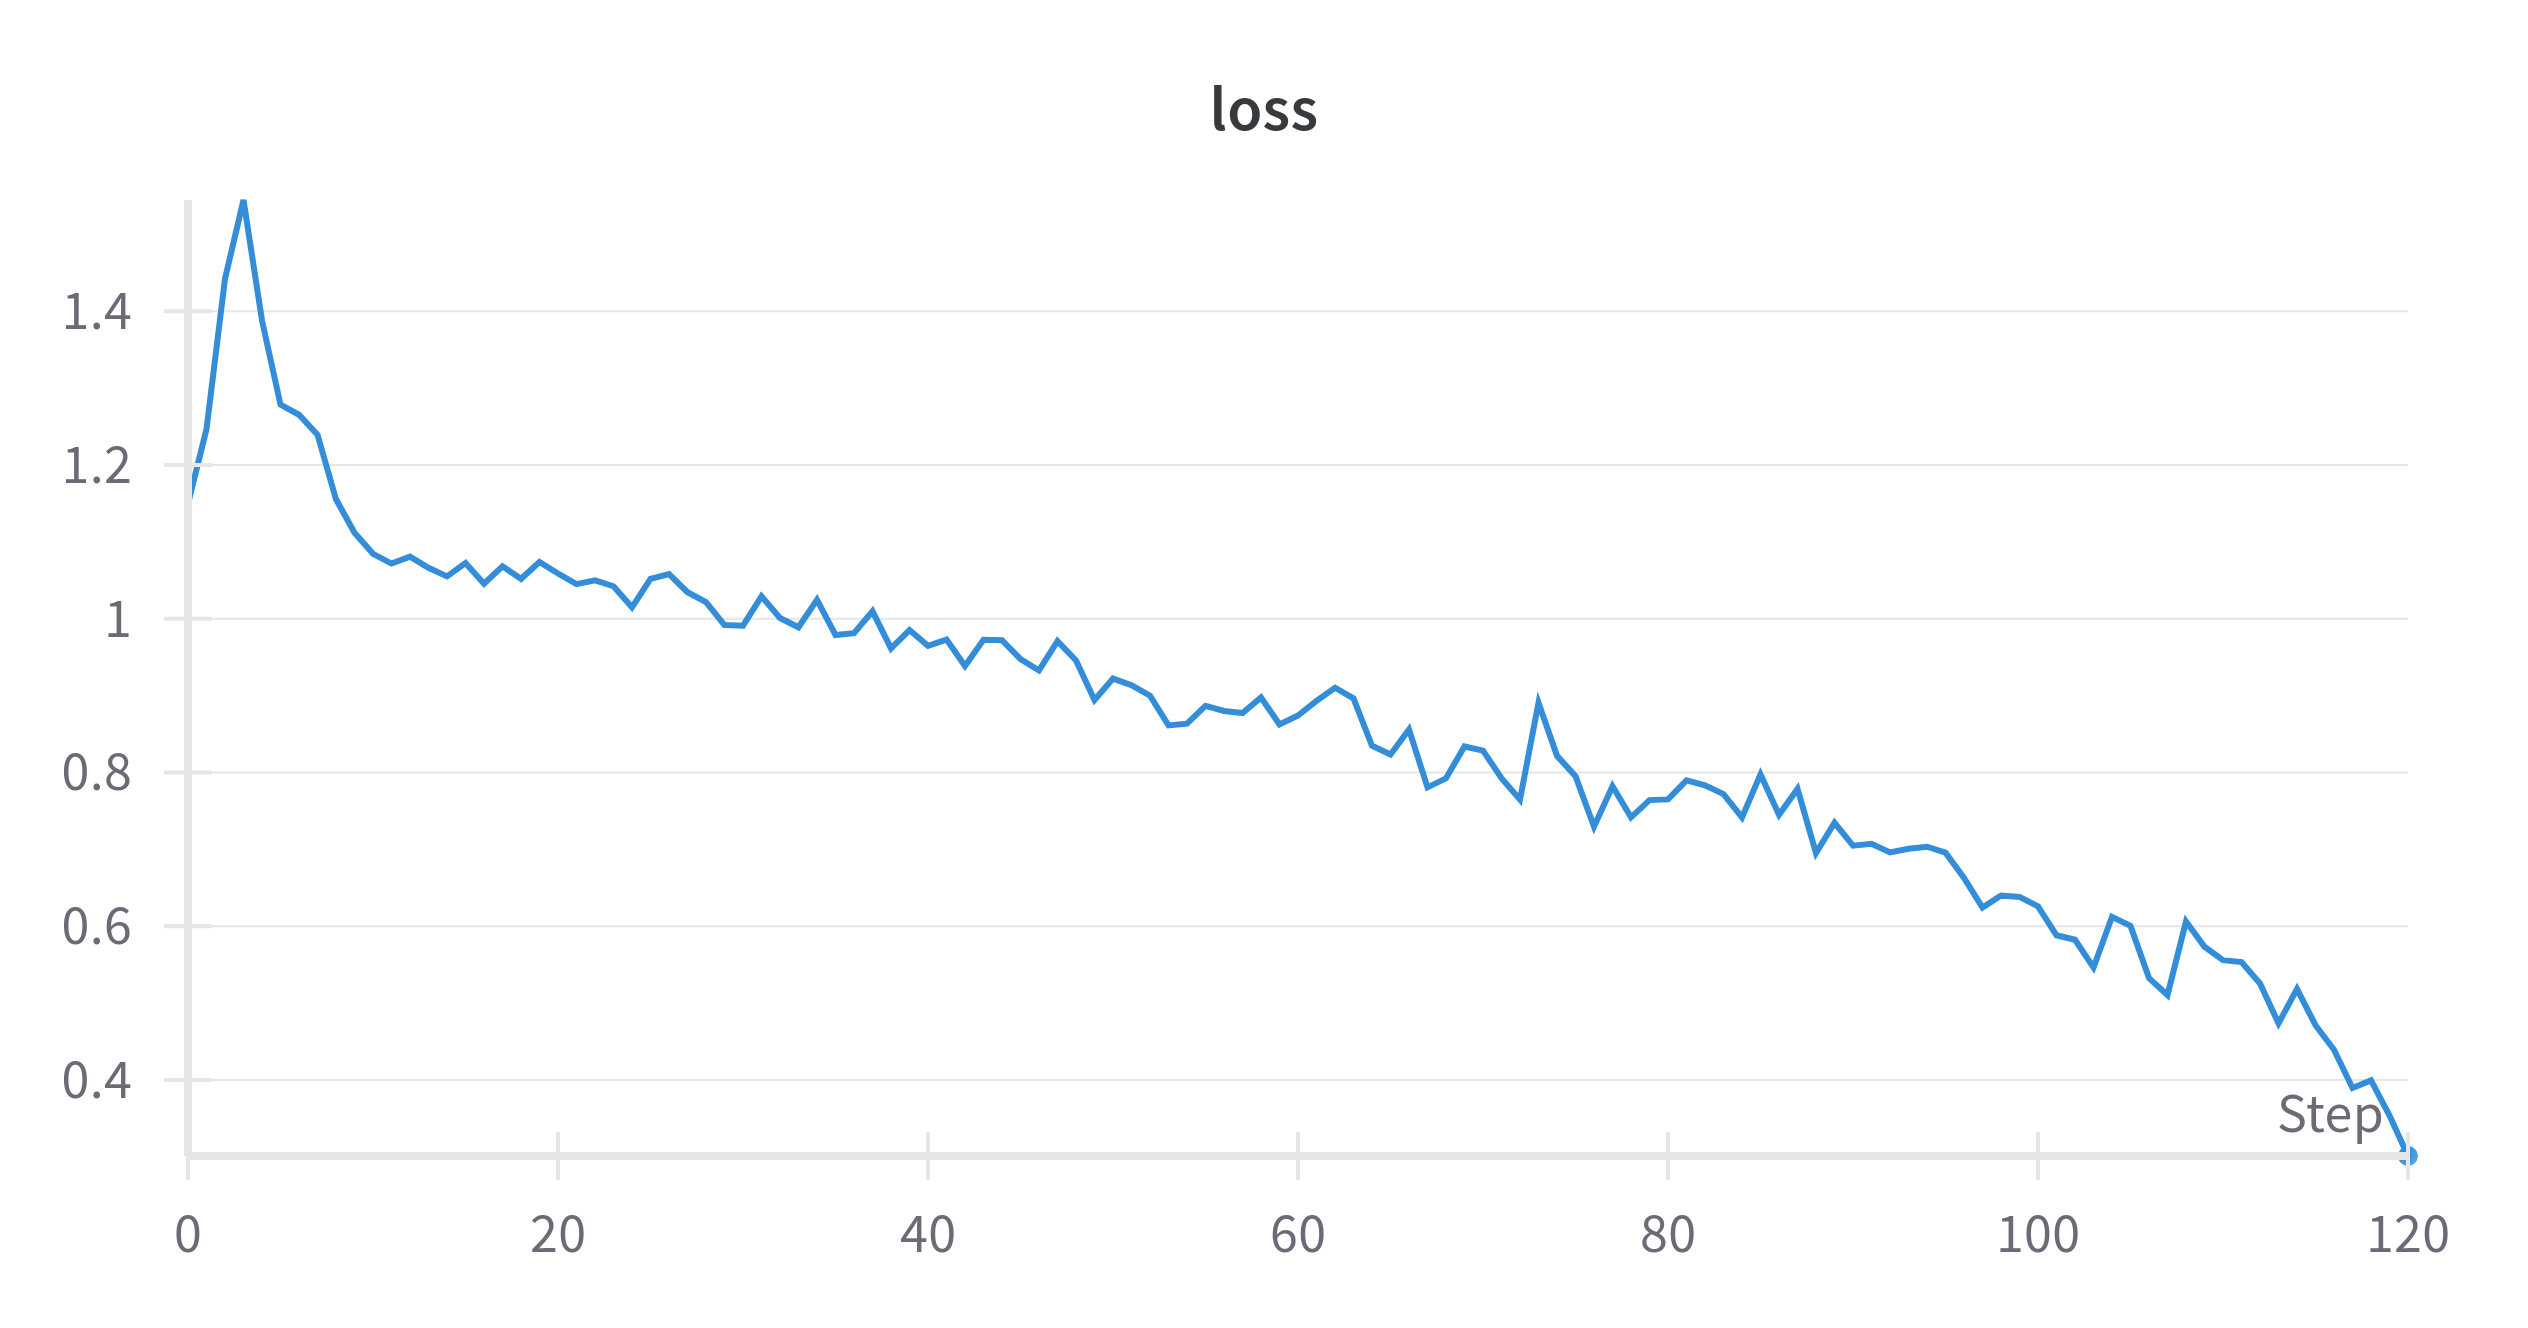
\includegraphics[width=\linewidth]{results/SAD-3-loss.png}
    \caption{
        Loss curve for SAD-3 Agent
    }
    \Description{Loss curve for SAD-3 Agent}
    \label{fig:sad3loss}
  \end{figure*}


% \subsection{Template Parameters}

% In addition to specifying the {\itshape template style} to be used in
% formatting your work, there are a number of {\itshape template parameters}
% which modify some part of the applied template style. A complete list
% of these parameters can be found in the {\itshape \LaTeX\ User's Guide.}

% Frequently-used parameters, or combinations of parameters, include:
% \begin{itemize}
% \item {\texttt{anonymous,review}}: Suitable for a ``double-anonymous''
%   conference submission. Anonymizes the work and includes line
%   numbers. Use with the \texttt{\acmSubmissionID} command to print the
%   submission's unique ID on each page of the work.
% \item{\texttt{authorversion}}: Produces a version of the work suitable
%   for posting by the author.
% \item{\texttt{screen}}: Produces colored hyperlinks.
% \end{itemize}

% This document uses the following string as the first command in the
% source file:
% \begin{verbatim}
% \documentclass[sigconf]{acmart}
% \end{verbatim}

% \section{Modifications}

% Modifying the template --- including but not limited to: adjusting
% margins, typeface sizes, line spacing, paragraph and list definitions,
% and the use of the \verb|\vspace| command to manually adjust the
% vertical spacing between elements of your work --- is not allowed.

% {\bfseries Your document will be returned to you for revision if
%   modifications are discovered.}

% \section{Typefaces}

% The ``\verb|acmart|'' document class requires the use of the
% ``Libertine'' typeface family. Your \TeX\ installation should include
% this set of packages. Please do not substitute other typefaces. The
% ``\verb|lmodern|'' and ``\verb|ltimes|'' packages should not be used,
% as they will override the built-in typeface families.

% \section{Title Information}

% The title of your work should use capital letters appropriately -
% \url{https://capitalizemytitle.com/} has useful rules for
% capitalization. Use the {\verb|title|} command to define the title of
% your work. If your work has a subtitle, define it with the
% {\verb|subtitle|} command.  Do not insert line breaks in your title.

% If your title is lengthy, you must define a short version to be used
% in the page headers, to prevent overlapping text. The \verb|title|
% command has a ``short title'' parameter:
% \begin{verbatim}
%   \title[short title]{full title}
% \end{verbatim}

% \section{Authors and Affiliations}

% Each author must be defined separately for accurate metadata
% identification.  As an exception, multiple authors may share one
% affiliation. Authors' names should not be abbreviated; use full first
% names wherever possible. Include authors' e-mail addresses whenever
% possible.

% Grouping authors' names or e-mail addresses, or providing an ``e-mail
% alias,'' as shown below, is not acceptable:
% \begin{verbatim}
%   \author{Brooke Aster, David Mehldau}
%   \email{dave,judy,steve@university.edu}
%   \email{firstname.lastname@phillips.org}
% \end{verbatim}

% The \verb|authornote| and \verb|authornotemark| commands allow a note
% to apply to multiple authors --- for example, if the first two authors
% of an article contributed equally to the work.

% If your author list is lengthy, you must define a shortened version of
% the list of authors to be used in the page headers, to prevent
% overlapping text. The following command should be placed just after
% the last \verb|\author{}| definition:
% \begin{verbatim}
%   \renewcommand{\shortauthors}{McCartney, et al.}
% \end{verbatim}
% Omitting this command will force the use of a concatenated list of all
% of the authors' names, which may result in overlapping text in the
% page headers.

% The article template's documentation, available at
% \url{https://www.acm.org/publications/proceedings-template}, has a
% complete explanation of these commands and tips for their effective
% use.

% Note that authors' addresses are mandatory for journal articles.

% \section{Rights Information}

% Authors of any work published by ACM will need to complete a rights
% form. Depending on the kind of work, and the rights management choice
% made by the author, this may be copyright transfer, permission,
% license, or an OA (open access) agreement.

% Regardless of the rights management choice, the author will receive a
% copy of the completed rights form once it has been submitted. This
% form contains \LaTeX\ commands that must be copied into the source
% document. When the document source is compiled, these commands and
% their parameters add formatted text to several areas of the final
% document:
% \begin{itemize}
% \item the ``ACM Reference Format'' text on the first page.
% \item the ``rights management'' text on the first page.
% \item the conference information in the page header(s).
% \end{itemize}

% Rights information is unique to the work; if you are preparing several
% works for an event, make sure to use the correct set of commands with
% each of the works.

% The ACM Reference Format text is required for all articles over one
% page in length, and is optional for one-page articles (abstracts).

% \section{CCS Concepts and User-Defined Keywords}

% Two elements of the ``acmart'' document class provide powerful
% taxonomic tools for you to help readers find your work in an online
% search.

% The ACM Computing Classification System ---
% \url{https://www.acm.org/publications/class-2012} --- is a set of
% classifiers and concepts that describe the computing
% discipline. Authors can select entries from this classification
% system, via \url{https://dl.acm.org/ccs/ccs.cfm}, and generate the
% commands to be included in the \LaTeX\ source.

% User-defined keywords are a comma-separated list of words and phrases
% of the authors' choosing, providing a more flexible way of describing
% the research being presented.

% CCS concepts and user-defined keywords are required for for all
% articles over two pages in length, and are optional for one- and
% two-page articles (or abstracts).

% \section{Sectioning Commands}

% Your work should use standard \LaTeX\ sectioning commands:
% \verb|section|, \verb|subsection|, \verb|subsubsection|, and
% \verb|paragraph|. They should be numbered; do not remove the numbering
% from the commands.

% Simulating a sectioning command by setting the first word or words of
% a paragraph in boldface or italicized text is {\bfseries not allowed.}

% \section{Tables}

% The ``\verb|acmart|'' document class includes the ``\verb|booktabs|''
% package --- \url{https://ctan.org/pkg/booktabs} --- for preparing
% high-quality tables.

% Table captions are placed {\itshape above} the table.

% Because tables cannot be split across pages, the best placement for
% them is typically the top of the page nearest their initial cite.  To
% ensure this proper ``floating'' placement of tables, use the
% environment \textbf{table} to enclose the table's contents and the
% table caption.  The contents of the table itself must go in the
% \textbf{tabular} environment, to be aligned properly in rows and
% columns, with the desired horizontal and vertical rules.  Again,
% detailed instructions on \textbf{tabular} material are found in the
% \textit{\LaTeX\ User's Guide}.

% Immediately following this sentence is the point at which
% % Table~\ref{tab:freq} is included in the input file; compare the
% placement of the table here with the table in the printed output of
% this document.



% To set a wider table, which takes up the whole width of the page's
% live area, use the environment \textbf{table*} to enclose the table's
% contents and the table caption.  As with a single-column table, this
% wide table will ``float'' to a location deemed more
% desirable. Immediately following this sentence is the point at which
% % Table~\ref{tab:commands} is included in the input file; again, it is
% instructive to compare the placement of the table here with the table
% in the printed output of this document.

% \begin{table*}
%   \caption{Some Typical Commands}
%   \label{tab:commands}
%   \begin{tabular}{ccl}
%     \toprule
%     Command &A Number & Comments\\
%     \midrule
%     \texttt{{\char'134}author} & 100& Author \\
%     \texttt{{\char'134}table}& 300 & For tables\\
%     \texttt{{\char'134}table*}& 400& For wider tables\\
%     \bottomrule
%   \end{tabular}
% \end{table*}

% Always use midrule to separate table header rows from data rows, and
% use it only for this purpose. This enables assistive technologies to
% recognise table headers and support their users in navigating tables
% more easily.

% \section{Math Equations}
% You may want to display math equations in three distinct styles:
% inline, numbered or non-numbered display.  Each of the three are
% discussed in the next sections.

% \subsection{Inline (In-text) Equations}
% A formula that appears in the running text is called an inline or
% in-text formula.  It is produced by the \textbf{math} environment,
% which can be invoked with the usual
% \texttt{{\char'134}begin\,\ldots{\char'134}end} construction or with
% the short form \texttt{\$\,\ldots\$}. You can use any of the symbols
% and structures, from $\alpha$ to $\omega$, available in
% \LaTeX~\cite{Lamport:LaTeX}; this section will simply show a few
% examples of in-text equations in context. Notice how this equation:
% \begin{math}
%   \lim_{n\rightarrow \infty}x=0
% \end{math},
% set here in in-line math style, looks slightly different when
% set in display style.  (See next section).

% \subsection{Display Equations}
% A numbered display equation---one set off by vertical space from the
% text and centered horizontally---is produced by the \textbf{equation}
% environment. An unnumbered display equation is produced by the
% \textbf{displaymath} environment.

% Again, in either environment, you can use any of the symbols and
% structures available in \LaTeX\@; this section will just give a couple
% of examples of display equations in context.  First, consider the
% equation, shown as an inline equation above:
% \begin{equation}
%   \lim_{n\rightarrow \infty}x=0
% \end{equation}
% Notice how it is formatted somewhat differently in
% the \textbf{displaymath}
% environment.  Now, we'll enter an unnumbered equation:
% \begin{displaymath}
%   \sum_{i=0}^{\infty} x + 1
% \end{displaymath}
% and follow it with another numbered equation:
% \begin{equation}
%   \sum_{i=0}^{\infty}x_i=\int_{0}^{\pi+2} f
% \end{equation}
% just to demonstrate \LaTeX's able handling of numbering.

% \section{Figures}

% The ``\verb|figure|'' environment should be used for figures. One or
% more images can be placed within a figure. If your figure contains
% third-party material, you must clearly identify it as such, as shown
% in the example below.
% \begin{figure}[h]
%   \centering
%   \includegraphics[width=\linewidth]{sample-franklin}
%   \caption{1907 Franklin Model D roadster. Photograph by Harris \&
%     Ewing, Inc. [Public domain], via Wikimedia
%     Commons. (\url{https://goo.gl/VLCRBB}).}
%   \Description{A woman and a girl in white dresses sit in an open car.}
% \end{figure}

% Your figures should contain a caption which describes the figure to
% the reader.

% Figure captions are placed {\itshape below} the figure.

% Every figure should also have a figure description unless it is purely
% decorative. These descriptions convey what’s in the image to someone
% who cannot see it. They are also used by search engine crawlers for
% indexing images, and when images cannot be loaded.

% A figure description must be unformatted plain text less than 2000
% characters long (including spaces).  {\bfseries Figure descriptions
%   should not repeat the figure caption – their purpose is to capture
%   important information that is not already provided in the caption or
%   the main text of the paper.} For figures that convey important and
% complex new information, a short text description may not be
% adequate. More complex alternative descriptions can be placed in an
% appendix and referenced in a short figure description. For example,
% provide a data table capturing the information in a bar chart, or a
% structured list representing a graph.  For additional information
% regarding how best to write figure descriptions and why doing this is
% so important, please see
% \url{https://www.acm.org/publications/taps/describing-figures/}.

% \subsection{The ``Teaser Figure''}

% A ``teaser figure'' is an image, or set of images in one figure, that
% are placed after all author and affiliation information, and before
% the body of the article, spanning the page. If you wish to have such a
% figure in your article, place the command immediately before the
% \verb|\maketitle| command:
% \begin{verbatim}
%   \begin{teaserfigure}
%     \includegraphics[width=\textwidth]{sampleteaser}
%     \caption{figure caption}
%     \Description{figure description}
%   \end{teaserfigure}
% \end{verbatim}

% \section{Citations and Bibliographies}

% The use of \BibTeX\ for the preparation and formatting of one's
% references is strongly recommended. Authors' names should be complete
% --- use full first names (``Donald E. Knuth'') not initials
% (``D. E. Knuth'') --- and the salient identifying features of a
% reference should be included: title, year, volume, number, pages,
% article DOI, etc.

% The bibliography is included in your source document with these two
% commands, placed just before the \verb|\end{document}| command:
% \begin{verbatim}
%   \bibliographystyle{ACM-Reference-Format}
%   \bibliography{bibfile}
% \end{verbatim}
% where ``\verb|bibfile|'' is the name, without the ``\verb|.bib|''
% suffix, of the \BibTeX\ file.

% Citations and references are numbered by default. A small number of
% ACM publications have citations and references formatted in the
% ``author year'' style; for these exceptions, please include this
% command in the {\bfseries preamble} (before the command
% ``\verb|\begin{document}|'') of your \LaTeX\ source:
% \begin{verbatim}
%   \citestyle{acmauthoryear}
% \end{verbatim}


%   Some examples.  A paginated journal article \cite{Abril07}, an
%   enumerated journal article \cite{Cohen07}, a reference to an entire
%   issue \cite{bardHanabiChallengeNew2020a}, a monograph (whole book) \cite{Kosiur01}, a
%   monograph/whole book in a series (see 2a in spec. document)
%   \cite{Harel79}, a divisible-book such as an anthology or compilation
%   \cite{Editor00} followed by the same example, however we only output
%   the series if the volume number is given \cite{Editor00a} (so
%   Editor00a's series should NOT be present since it has no vol. no.),
%   a chapter in a divisible book \cite{Spector90}, a chapter in a
%   divisible book in a series \cite{Douglass98}, a multi-volume work as
%   book \cite{Knuth97}, a couple of articles in a proceedings (of a
%   conference, symposium, workshop for example) (paginated proceedings
%   article) \cite{Andler79, Hagerup1993}, a proceedings article with
%   all possible elements \cite{Smith10}, an example of an enumerated
%   proceedings article \cite{VanGundy07}, an informally published work
%   \cite{Harel78}, a couple of preprints \cite{Bornmann2019,
%     AnzarootPBM14}, a doctoral dissertation \cite{Clarkson85}, a
%   master's thesis: \cite{anisi03}, an online document / world wide web
%   resource \cite{Thornburg01, Ablamowicz07, Poker06}, a video game
%   (Case 1) \cite{Obama08} and (Case 2) \cite{Novak03} and \cite{Lee05}
%   and (Case 3) a patent \cite{JoeScientist001}, work accepted for
%   publication \cite{rous08}, 'YYYYb'-test for prolific author
%   \cite{SaeediMEJ10} and \cite{SaeediJETC10}. Other cites might
%   contain 'duplicate' DOI and URLs (some SIAM articles)
%   \cite{Kirschmer:2010:AEI:1958016.1958018}. Boris / Barbara Beeton:
%   multi-volume works as books \cite{MR781536} and \cite{MR781537}. A
%   couple of citations with DOIs:
%   \cite{2004:ITE:1009386.1010128,Kirschmer:2010:AEI:1958016.1958018}. Online
%   citations: \cite{TUGInstmem, Thornburg01, CTANacmart}.
%   Artifacts: \cite{R} and \cite{UMassCitations}.

% \section{Acknowledgments}

% Identification of funding sources and other support, and thanks to
% individuals and groups that assisted in the research and the
% preparation of the work should be included in an acknowledgment
% section, which is placed just before the reference section in your
% document.

% This section has a special environment:
% \begin{verbatim}
%   \begin{acks}
%   ...
%   \end{acks}
% \end{verbatim}
% so that the information contained therein can be more easily collected
% during the article metadata extraction phase, and to ensure
% consistency in the spelling of the section heading.

% Authors should not prepare this section as a numbered or unnumbered {\verb|\section|}; please use the ``{\verb|acks|}'' environment.

% \section{Appendices}

% If your work needs an appendix, add it before the
% ``\verb|\end{document}|'' command at the conclusion of your source
% document.

% Start the appendix with the ``\verb|appendix|'' command:
% \begin{verbatim}
%   \appendix
% \end{verbatim}
% and note that in the appendix, sections are lettered, not
% numbered. This document has two appendices, demonstrating the section
% and subsection identification method.

% \section{Multi-language papers}

% Papers may be written in languages other than English or include
% titles, subtitles, keywords and abstracts in different languages (as a
% rule, a paper in a language other than English should include an
% English title and an English abstract).  Use \verb|language=...| for
% every language used in the paper.  The last language indicated is the
% main language of the paper.  For example, a French paper with
% additional titles and abstracts in English and German may start with
% the following command
% \begin{verbatim}
% \documentclass[sigconf, language=english, language=german,
%                language=french]{acmart}
% \end{verbatim}

% The title, subtitle, keywords and abstract will be typeset in the main
% language of the paper.  The commands \verb|\translatedXXX|, \verb|XXX|
% begin title, subtitle and keywords, can be used to set these elements
% in the other languages.  The environment \verb|translatedabstract| is
% used to set the translation of the abstract.  These commands and
% environment have a mandatory first argument: the language of the
% second argument.  See \verb|sample-sigconf-i13n.tex| file for examples
% of their usage.

% \section{SIGCHI Extended Abstracts}

% The ``\verb|sigchi-a|'' template style (available only in \LaTeX\ and
% not in Word) produces a landscape-orientation formatted article, with
% a wide left margin. Three environments are available for use with the
% ``\verb|sigchi-a|'' template style, and produce formatted output in
% the margin:
% \begin{description}
% \item[\texttt{sidebar}:]  Place formatted text in the margin.
% \item[\texttt{marginfigure}:] Place a figure in the margin.
% \item[\texttt{margintable}:] Place a table in the margin.
% \end{description}

% %%
% %% The acknowledgments section is defined using the "acks" environment
% %% (and NOT an unnumbered section). This ensures the proper
% %% identification of the section in the article metadata, and the
% %% consistent spelling of the heading.
% \begin{acks}
% To Robert, for the bagels and explaining CMYK and color spaces.
% \end{acks}

%%
%% The next two lines define the bibliography style to be used, and
%% the bibliography file.
% \bibliographystyle{ACM-Reference-Format}
% \bibliography{honors}
% \printbibliography

%%
%% If your work has an appendix, this is the place to put it.
% \appendix

% \section{Research Methods}

% \subsection{Part One}

% Lorem ipsum dolor sit amet, consectetur adipiscing elit. Morbi
% malesuada, quam in pulvinar varius, metus nunc fermentum urna, id
% sollicitudin purus odio sit amet enim. Aliquam ullamcorper eu ipsum
% vel mollis. Curabitur quis dictum nisl. Phasellus vel semper risus, et
% lacinia dolor. Integer ultricies commodo sem nec semper.

% \subsection{Part Two}

% Etiam commodo feugiat nisl pulvinar pellentesque. Etiam auctor sodales
% ligula, non varius nibh pulvinar semper. Suspendisse nec lectus non
% ipsum convallis congue hendrerit vitae sapien. Donec at laoreet
% eros. Vivamus non purus placerat, scelerisque diam eu, cursus
% ante. Etiam aliquam tortor auctor efficitur mattis.

% \section{Online Resources}

% Nam id fermentum dui. Suspendisse sagittis tortor a nulla mollis, in
% pulvinar ex pretium. Sed interdum orci quis metus euismod, et sagittis
% enim maximus. Vestibulum gravida massa ut felis suscipit
% congue. Quisque mattis elit a risus ultrices commodo venenatis eget
% dui. Etiam sagittis eleifend elementum.

% Nam interdum magna at lectus dignissim, ac dignissim lorem
% rhoncus. Maecenas eu arcu ac neque placerat aliquam. Nunc pulvinar
% massa et mattis lacinia.

\end{document}
\endinput
%%
%% End of file `sample-sigconf.tex'.
